\documentclass[letterpaper,12pt]{article}
\usepackage{tabularx} % extra features for tabular environment
\usepackage{amsmath}  % improve math presentation
\usepackage{graphicx, subcaption} % takes care of graphic including machinery
\usepackage[margin=1in,letterpaper]{geometry} % decreases margins
\usepackage{xspace}
\usepackage{ANA-FTAG-2020-08-PAPER-defs}
\usepackage[style=numeric, sorting=none]{biblatex}
\addbibresource{ANA-FTAG-2020-08-PAPER.bib}
\addbibresource{bib/ATLAS.bib}
\addbibresource{bib/ATLAS-useful.bib}
\addbibresource{bib/PubNotes.bib}
\addbibresource{bib/ConfNotes.bib}
\addbibresource{bib/ATLAS-SUSY.bib}

\usepackage[final]{hyperref} % adds hyper links inside the generated pdf file
\usepackage[T1]{fontenc}
\usepackage{setspace}
\usepackage{float}
\usepackage{makeidx}
\usepackage{titlesec}

\newcommand\bjetineq{\mathop{\mbox{$b$ $\rm{jet}$}}}
\newcommand\bjetunder{\mathop{\footnotesize{\mbox{$b$ $\rm{jet}$}}}\normalsize}
\newcommand\cjetineq{\mathop{\mbox{$c$ $\rm{jet}$}}}
\newcommand\cjetunder{\mathop{\footnotesize{\mbox{$c$ $\rm{jet}$}}}\normalsize}
\setcounter{secnumdepth}{4}
\newcommand{\specialcell}[2][c]{%
  \begin{tabular}[#1]{@{}c@{}}#2\end{tabular}}

\titleformat{\paragraph}
{\normalfont\normalsize\bfseries}{\theparagraph}{1em}{}
\titlespacing*{\paragraph}
{0pt}{3.25ex plus 1ex minus .2ex}{1.5ex plus .2ex}
\restylefloat*{figure}
\hypersetup{
	colorlinks=true,       % false: boxed links; true: colored links
	linkcolor=blue,        % color of internal links
	citecolor=blue,        % color of links to bibliography
	filecolor=magenta,     % color of file links
	urlcolor=blue         
}

%++++++++++++++++++++++++++++++++++++++++
\linespread{1.17}
\makeindex
\begin{document}


\title{Search for Higgs boson pair-production in the $bb\tau\tau$ final state using proton-proton collisions at $\sqrt{s}$ = 13 \TeV\ data with the ATLAS detector}%Fake Factors Calculation and Implementation in H$\rightarrow$ bb$\tau^+\tau^-$ analysis with MC16a/MC16d in Release 21 with the ATLAS detector
\author{ Zhiyuan Li}
\date{\today}
\maketitle
\begin{figure}[htp]
\centering

\includegraphics[width=.5\textwidth]{logo.png}
\vspace{3em}
\centering

\includegraphics[width=.45\textwidth]{ATLAS-Logo-Ref-RGB-H_1.jpg}
\end{figure}
\newpage


\tableofcontents{}
\printindex{}


\newpage
\section{Introduction}
\section{Theory and Motivation}
\subsection{The Standard Model and the Higgs boson}
\subsection{Beyond the Standard Model}
\section{The ATLAS experiment at the Large Hadron Collider}
\subsection{The Large Hadron Collider}

The Large Hadron Collider \cite{Evans:2008zzb} is the world's largest and most powerful particle accelerator. 
It started in 2008 and remains its crucial role in the many accelerators at CERN and in the world.
The main body of the collider consists of a ring tunnel of perimeter of 26.7 km, with 
superconducting magnets along the tunnel to keep the particle beam in direction
 and a large number of accelerating structures to boost the beam to the desired energy.

Inside the tunnel, two beams of particles travelling at close to the speed of light 
in opposite direction are made to collide. These two beams are kept in separate beam pipes,
cooled to $-271.3^\circ C$ ($1.9K$) with liquid helium distributed by dedicated system, 
 and ultra-high vacuum, a vacuum thinner than 
interstellar void, matianed for 48 km of low-temperature section and 6 km of room-temperature 
section. 

Thousands of magnets are used to direct the beams along the beam pipe, either to bend the beams or
to focus. The particles are so small that making them collide is akin to 
firing two needles 10 kilometers away and meet halfway. 

All the controls for the accelerator, its services and technical infrastructure 
are located at the CERN Control Centre. 
From here, the beams inside the LHC are made to collide at four locations around the accelerator ring, 
corresponding to the positions of four particle detectors – ATLAS (A Toroidal LHC ApparatuS) \cite{PERF-2007-01}, 
CMS [S08004] (Compact Muon Solenoid), ALICE (A Large Ion Collider Experiment) [S08002] 
and LHCb (b stands for beauty) [S08005].


	\subsubsection{Design and performance}

	The LHC is a two-ring-superconducting-hadron accelerator and collider
	installed in the existing 26.7 km tunnel that was constructed between 1984 and 1989 
	for the CERN LEP machine. The LEP tunnel has eight straight sections and eight arcs 
	and lies between 45 m and 170 m below the surface on a plane inclined at 1.4\% sloping towards the Léman lake.
	Approximately 90\% of its length is in molasse rock, which has excellent characteristics for this application,
	and 10\% is in limestone under the Jura mountain. There are two transfer tunnels, 
	each approxi-mately 2.5 km in length, linking the LHC to the CERN accelerator complex that acts as injector.
	As mentioned before, the beam piples are maintained in vacuum for low and high temperature section.
	For the low temperature section, the vacuum is achieved by pumping in 9000 $m^3$ of cryogenic
	gas, which later will be condensed and adhered to the surface of the beampipe. For the room temperature
	section, the vacuum is achieved by use of non-evaporable getter (NEG) that absorbs residue gas particles 
	when heated. More residue is absorbed by ion pumper. 

	Being a proton-proton (pp) collider, there are advantages and disadvantages compared to a
	proton-anti-proton collider and an electron-positron collider. 
	Two rings are needed to accommodate the two counter-rotatign beams, unlike particle-antiparticle 
	colliders that can have both beams sharing the same phase space in a single ring.
	However it would not be possible to to achieve such high luminosity using
	anti-proton beams. 
	In principle, the mass of the proton is much larger than the mass of the electron, the
	synchrotron radiation losses will be much smaller, and the long straight sections designed for
	compensate the losses (as designed in the LEP) can be reduced. However these sections are kept 
	as the LEP has as a cost-effective solution. 
	The tunnel in the arcs has a finished internal diameter of 3.7 m, 
	due to the technical difficulties to install two separate rings in such small space,
	LHC adopted the twin-bore magnet design, as shown in Figure \ref{fig:double_bore_magnet}.
	It was proposed by John Blewett at the Brookhaven laboratory in 1971 first for
	cost consideration [J.P. Blewett, 200GeV intersecting storage accelerators,Proceedings of the8thInternationalConference on High-Energy Accelerators, CERN, Geneva Switzerland (1971)],
	but in the case of the LHC the overriding reason for adopting this solution
	is the lack of space in the tunnel. 

	\includegraphics[width=1\textwidth]
	\begin{figure}[]
		\begin{centering}	
		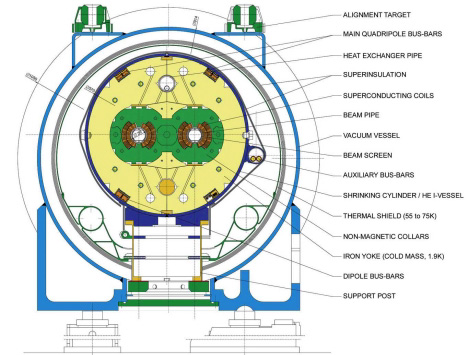
\includegraphics[width=.4\textwidth]{Detector plots/LHC-double-bore-magnet.jpg}
		\caption{ Double-bore magnet configuration of the LHC superconducting magnets.[THE LHC SUPERCONDUCTING MAGNETSL. Rossi, Accelerator Technology Division, CERN, Geneva, Switzerland]
			}
		\label{fig:accelerator_complex}
		\end{centering}
	\end{figure}

	The aim of the LHC is to reveal the physics beyond the Standard Model with centre of mass 
	collision energies of up to 14 TeV.
	The number of events per second generated in the LHC collisionsis given by:
	\[
		N_{event} = L\sigma_{event}\],

	where $\sigma_event$ is the cross section for the event under study and $L$ the machine luminosity. 
	The machine luminosity depends on the beam parameters and can be written for a Gaussian beam distribution as:
	\[
	L = \frac{N_b^2 n_b f_{rev} \gamma_r}{4\pi \epsilon_n \beta*} F	
	\],

	where$N_b$is the number of particles per bunch,$n_b$the number of bunches per beam,$f_rev$ 
	the revolution frequency, $\gamma_r$ the relativistic gamma factor, $\epsilon_r$ 
	the normalized transverse beam emittance, $\beta*$ the beta function at the collision point which
	describes the size of the beam, and	$F$ the geometric luminosity reduction factor due to the 
	crossing angle at the interaction point (IP).

	The two high luminosity experiments, ATLAS and CMS are
	both aiming at a peak luminosity of $L$ = $10^{34}cm^2s^1$ for proton operation.
	The two low luminosity experiments: LHCB for 
	B-physics, is aiming at a peak luminosity of $L$ = $10^{32}cm^2s^1$, 
	and the dedicated ion experiment, ALICE, is aiming at apeak luminosity of
	$L$ = $10^{27}cm^2s^1$ for nominal lead-lead ion operation.

	To reach such high energies, a series of acceleration is required for the beams before
	entering the LHC ring. The protons are supplied by the injector chain 
	Linac2 — Proton Synchrotron Booster (PSB) — Proton Synchrotron (PS) — Super Proton Synchrotron (SPS), 
	as shown in Figure \ref{fig:accelerator_complex}, 
	reaching an energy of 450 GeV when leaving the SPS. 
	Each proton beam contains 2808 "bunches" of approximately 1.15 \times 10$^11$ protons, arranded in 
	"trains" of bunches with 72 bunches each "carriage". Inside the "carriage", each beam has
	a spacing of 24.95 ns and between each "carriage" there is a gap of ~ 320 ns. The beams are also 
	required to have well defined transverse and longitudinal emittance. 



	\includegraphics[width=1\textwidth]
	\begin{figure}[]
		\begin{centering}	
		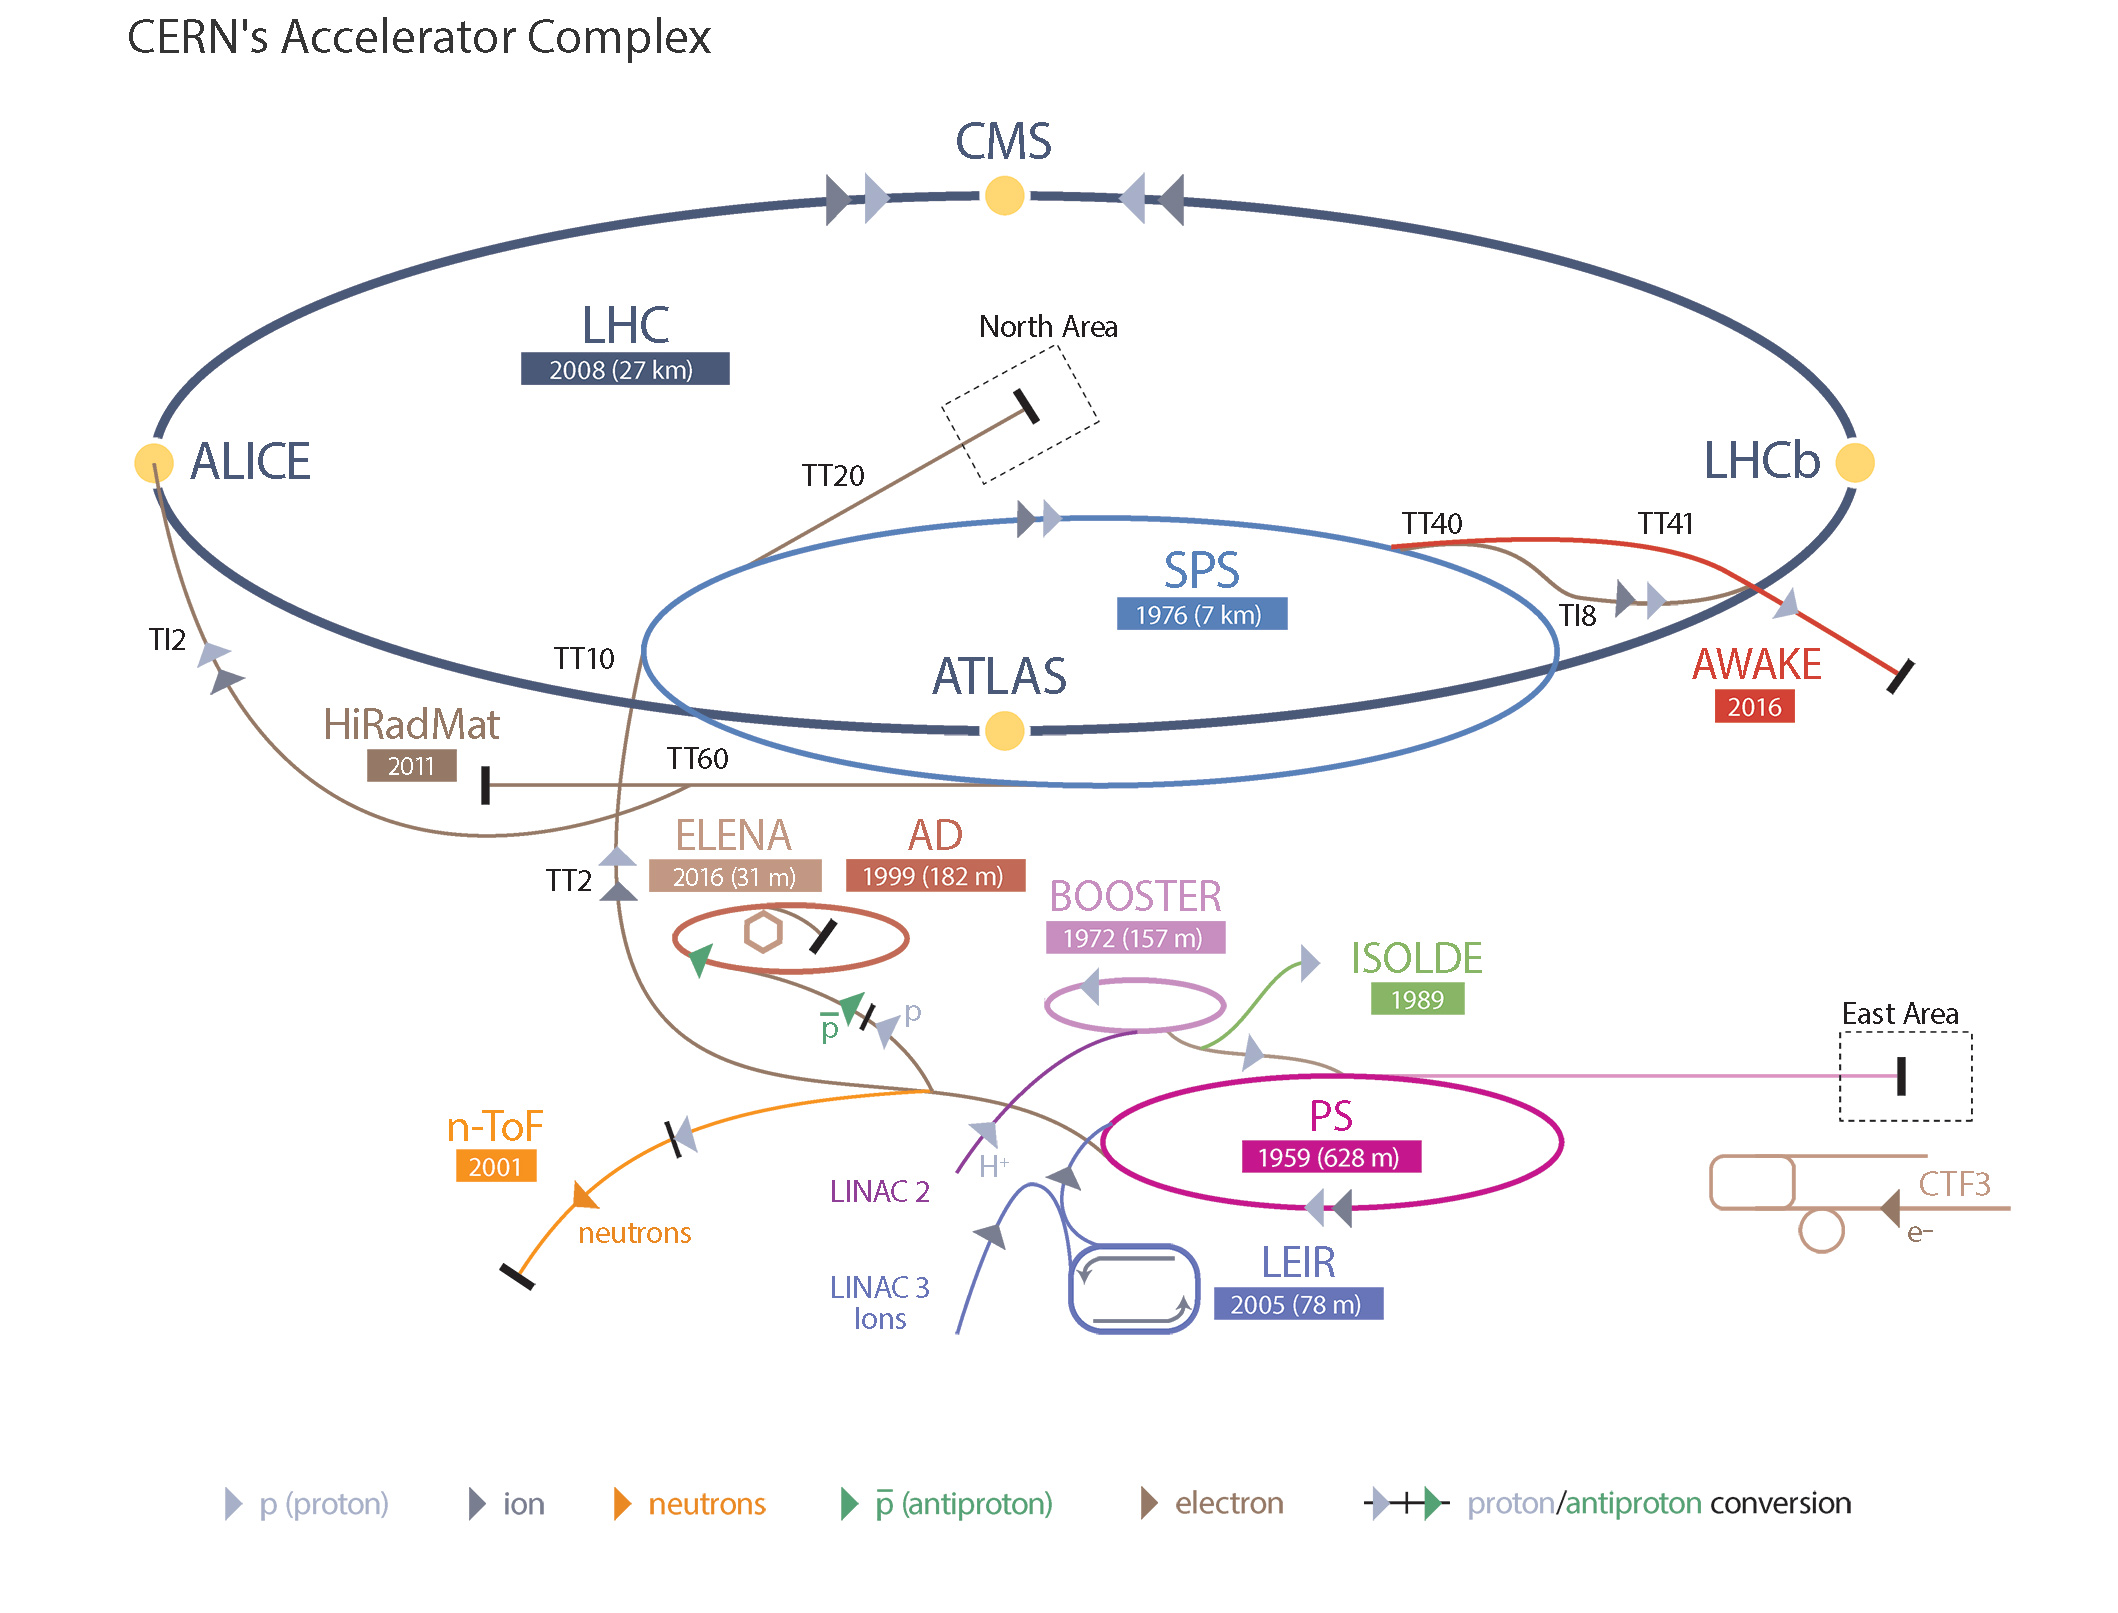
\includegraphics[width=.4\textwidth]{Detector plots/accelerator_complex.png}
		\caption{The LHC is the last ring (dark blue line) in a complex chain of 
		particle accelerators. The smaller machines are used in a chain to help boost 
		the particles to their final energies and provide beams to a whole set of smaller experiments.
			}
		\label{fig:double_bore_magnet}
		\end{centering}
	\end{figure}


	\subsubsection{Runs and results}
	Following the downtime after an incident in one of the main dipole circuits 
	during the first commissioning in 2008 [3],
	the operation restarted at lower beam energy to minimize the risk. 
	Therefore, the first proton run (2010-2013) [4–6] was
	carried out at 3.5–4 TeV (centre of mass energy 7-8 TeV). Furthermore, a bunch spacing
	of 50 ns was used instead of the nominal 25 ns. 
	This implied fewer bunches with larger intensity and hence a 
	high peak luminosity (0.8 \times 10$^{34}$ cm$^{-2}$s$^{-1}$ still smaller than
	the nominal 10$^{34}$ cm$^{-2}$s$^{-1}$ luminosity) but larger than nominal pileup. 
	Run 1 resulted in about 30 \fb of proton data and important physics results,
	most notably the discovery of the Higgs boson [7,8].
	Run 1 was followed by a long shutdown (LS1, 2013–2014)
	with a large number of consolidation and upgrade activities [9]. 	
	The bus-bar splices between the superconducting magnets were improved, 
	in order to make sure that the LHC could operate at higher energy 
	without risk of repeating the 2008 incident. 

	\includegraphics[width=1\textwidth]
	\begin{figure}[]
		\begin{centering}	
		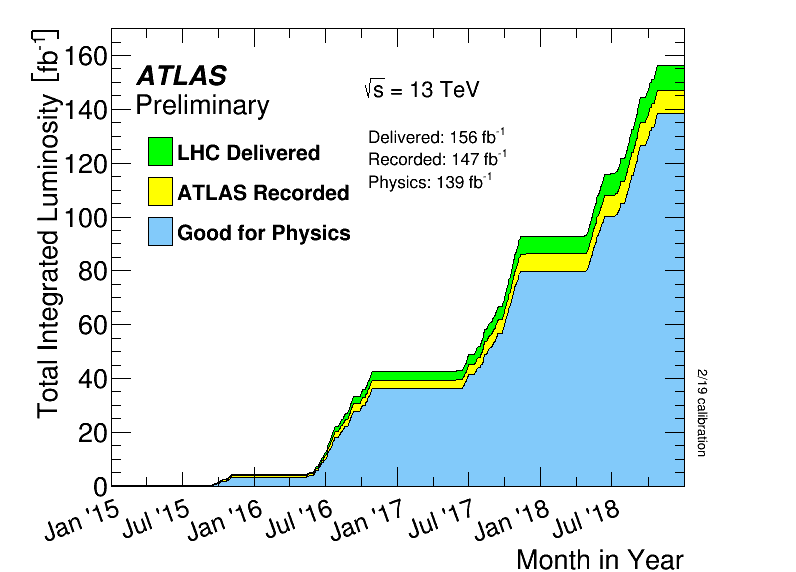
\includegraphics[width=.4\textwidth]{Detector plots/Run2_lumi.png.png}
		\caption{Cumulative luminosity versus time delivered to 
		ATLAS (green), recorded by ATLAS (yellow), and certified to be 
		good quality data (blue) during stable beams for pp collisions 
		at 13 TeV centre-of-mass energy in Run 2. 
			}
		\label{fig:Run2_lumi}
		\end{centering}
	\end{figure}

	Run 2 (2016-2018) was carried out
	at 6.5 TeV (center of mass energy 13 TeV) [cite the correct run  2 paper]. 
	As shown in Figure \ref{fig:Run2_lumi}, out of the 156 \fb of data LHC has delivered, the ATLAS detector has recorded 
	147 \fb and \lumi of data is certified to be good quality data.
	The delivered luminosity accounts for the luminosity delivered from the start of 
	stable beams until the LHC requests ATLAS to put the detector in a 
	safe standby mode to allow a beam dump or beam studies. 
	The recorded luminosity is slightly smaller than the delivered luminosity, due 
	to the inefficiency of the Data Acquisition (DAQ) and the so called "warm start": 
	when the stable beam flag is raised, 
	the tracking detectors undergo a ramp of the high-voltage and, 
	for the pixel system, turning on the preamplifiers. 
	More details of the ATLAS detector can be found in the following sections. 
	The recorded data is checked carefully to exclude possible hardware or software  issues. 
	This is achieved by monitoring detector-level quantities 
	and reconstructed collision event characteristics at key stages of the data processing chain.
	This procedure led to high efficiency of good quality data: 95.6\%.	[cite  JINST 15 (2020) P04003,  arXiv:1911.04632]

	In this thesis the \lumi data recorded by the ATLAS detector of Run 2 is used.
	The nominal bunch spacing of 25 ns was used, with slightly less bunches (2500) each beam.
	The LHC experts have continually improved the running scenario to increase the luminosity,
	and during Run 2 the luminosity surpassed the designed luminosity by a factor of 2. 
	As well as improving the instantaneous luminosity, the availability of the machine
	was dramatically improved during Run 2 which is an important factor enabling the high efficiency 
	of good quality data as mentioned above.
	During Run 2, the machine was providing physics collisions during 50\% of 
	the allocated physics time, which is very impressive for a super conducting collider. 
	An important parameter for the LHC experiments is the pileup, 
	which is determined by the luminosity per bunch, and is a measure of 
	the number of inelastic pp interactions that occur per bunch crossing. 
	Higher pileup gives more luminosity (for a fixed number ofbunches) 
	but makes physics analysis more difficult due to the signals in the detector 
	from the additional interactions. The distribution of the recorded luminosity over
	the pileup is shown in Figure \ref{fig:Run2_pileup}. It's a challenging task for the 
	trigger and reconstruction algorithms to achieve robustness under such high pileup 
	condition.



	\includegraphics[width=1\textwidth]
	\begin{figure}[]
		\begin{centering}	
		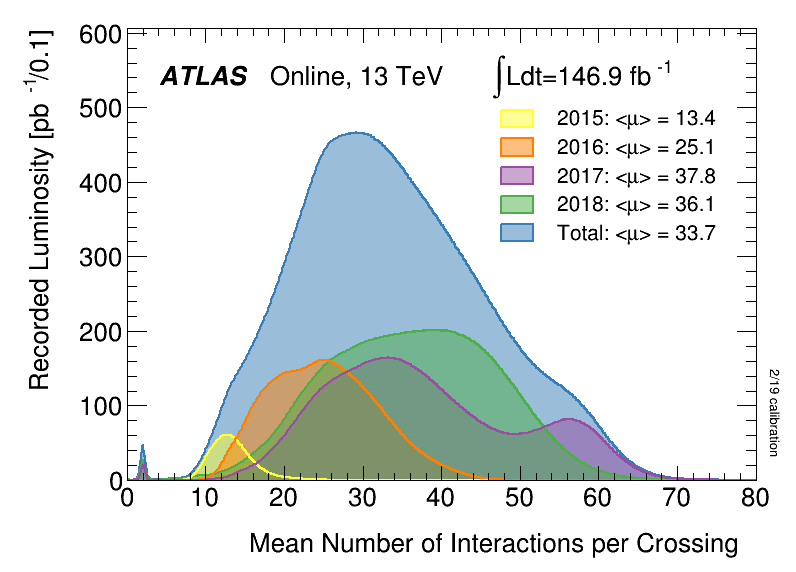
\includegraphics[width=.4\textwidth]{Detector plots/Run2_pileup.png}
		\caption{ Shown is the luminosity-weighted distribution of the mean number of 
		interactions per crossing for the Run 2 data. All data recorded by ATLAS during 
		stable beams is shown, and the integrated luminosity and the mean mu value are given in the figure. 
			}
		\label{fig:Run2_pileup}
		\end{centering}
	\end{figure}




\subsection{The ATLAS Detector}







\section{Data and Monte Carlo samples}
\section{Physics Objects Reconstruction}
\subsection{Track and vertex}
\subsection{Electron}
\subsection{Muon}
\subsection{Jet}
\subsection{\bjets}


\subsubsection{Flavour tagging}
\label{sec:Flavour tagging}

The identification of jets containing $b$-hadrons (\bjets) 
against the large background of jets containing $c$-hadrons 
(\cjets) or coming from the hadronization of light ($u$,$d$,$s$) 
quarks or gluons is of major importance in many areas of the 
physics programme of the ATLAS experiment at the LHC. 
It is crucial in a large number of Standard Model (SM) 
precision measurements, studies of the Higgs boson properties, and 
searches for new phenomena \cite{SUSY-2014-08, ATLAS-CONF-2018-043,Interpreting_Higgs_result}.
It also plays an important role in 
the $HH \to bb\tau\tau$ searches presenting in Chapter \ref{sec:search for dihiggs}. 
% as well as the recent 
% observation of the Higgs boson decay into bottom quarks \cite{HIGG-2018-04} 
% and of its production in association with a top-quark pair \cite{HIGG-2018-13}. 


The ATLAS Collaboration uses various algorithms to identify 
\bjets \cite{PERF-2012-04}, referred to as \btagging\ algorithms, 
when analysing data recorded during Run 2 of the LHC. These 
algorithms exploit the long lifetime, high mass and high decay 
multiplicity of $b$-hadrons, as well as the properties of the \bquark\  
fragmentation. Given a lifetime of the order of 1.5 ps, $b$-hadrons have a 
significant mean flight length ($\langle c\tau \rangle$ $\approx$ 450 $\mu m$), 
in the detector before decaying, generally leading to at least one vertex 
displaced from the hard-scatter collision point, as illustrated in Figure~\ref{fig:b-jet-decay}.

\begin{figure}[]
	\begin{centering}	
	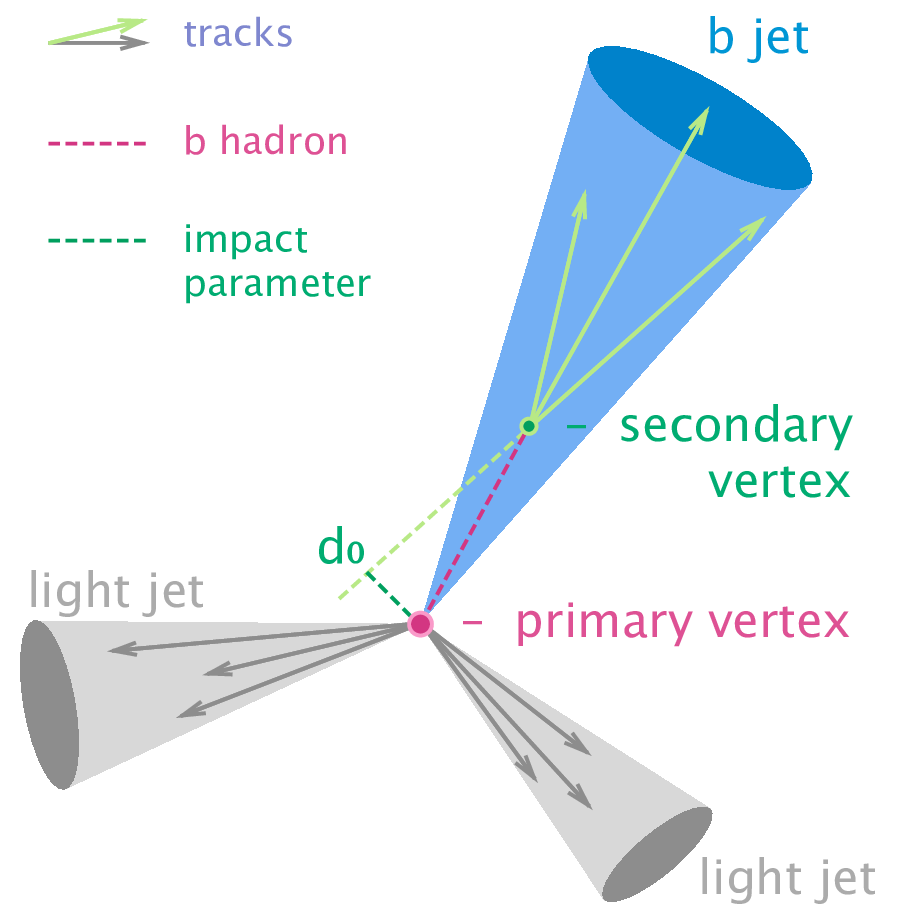
\includegraphics[width=.4\textwidth]{FTAG_plots/B-tagging_diagram.png}
	\caption{A diagram showning the b hadron decay initiated jets. }
	\label{fig:b-jet-decay}
	\end{centering}
\end{figure}


The strategy developed by the ATLAS Collaboration is based on a two-stage approach. 
Firstly, low-level algorithms reconstruct the characteristic features of 
the \bjets via two complementary approaches, one that uses the 
individual properties of charged-particle tracks, later referred 
to as tracks, associated with a hadronic jet, and a second which 
combines the tracks to explicitly reconstruct displaced vertices. 
These algorithms, first introduced during Run 1 \cite{PERF-2012-04}, 
have been improved and retuned for Run 2 \cite{FTAG-2018-01}. 
Secondly, in order to 
maximise the \btagging\ performance, the results of the low-level 
\btagging\ algorithms are combined into high-level algorithms 
via multivariate classifiers. 


The most performant algorithms presently in use in physics 
analyses at ATLAS are based on multivariate combinations 
of the available information (MV2) or additionally using a
deep feed-forward neural network (DL1) \cite{tagging,ATL-PHYS-PUB-2017-013}, 
as shown in Figure \ref{fig:b-tagging-performance}, where the performance
is characterised by the probability of 
tagging a \bjet\ (\bjet\ tagging efficiency, 
$\epsilon_b$) and the probability of mistakenly identifying 
a \cjet or a light-flavour jet as a \bjet\, 
labelled $\epsilon_c$($\epsilon_l$). 
In addition, the distribution of the output discriminant
of the MV2 and DL1 tagger for \bjet, \cjet, and light-flavour jets
in the \ttbar\ simulated events are shown in Figure~\ref{fig:b-tagging-score}.
Depending on the low-level algorithm, 
the DL1 tagger can be further separated into two taggers: DL1 and DL1r,
 where the DL1 tagger uses traditional track-based impact parameter 
 taggers IP2D and IP3D \cite{ATL-PHYS-PUB-2016-012} 
 and the DL1r tagger uses a Recurrent Neural Network Impact Parameter tagger 
 (RNNIP) \cite{ATL-PHYS-PUB-2017-013}. The DL1r tagger is now the 
 default \btagging\ algorithm used for flavour tagging in ATLAS.
 The performance of the algorithms is quantified 
in terms of \cjet\ (light jet) rejections, defined as 
1/$\epsilon_c$ and 1/$\epsilon_l$. 
%Their high mass also leads to decay products with a larger transverse momentum relative to the jet axis with respect to the ones typically found in jets from light partons. Finally, heavy hadrons have a sizable branching ratio for semileptonic decays, hence the presence of soft leptons in the produced jets provides another tool for heavy jet identification. %The general strategy is to start with simple algorithms that exploits a particular property of b jets and progressively add more information to build moresophisticated algorithms. %The output of these algorithms consists in a discriminant value for each jet. Operating points are then defined as thresholds on the discriminant, designed to provide a determined efficiency for identifying b jets.
% Low-level $b$-taggingalgorithms fall into two broad categories. A first approach, implemented in the IP2D and IP3D algorithms \cite{ATL-PHYS-PUB-2017-013}, or RNNIP \cite{ATL-PHYS-PUB-2017-003} is inclusive and based on exploiting the large impact parameters of the tracks originating from the $b$-hadron decay. The second approach explicitly reconstructs displaced vertices. To maximise the $b$-tagging performance, low-level algorithm results are combined using multivariate classifiers. To this end, two high-level tagging algorithms have been developed. The first one,MV2\cite{ATL-PHYS-PUB-2017-013}, is based on a boosted decisiontree (BDT) discriminant, while the second one,DL1, is based on a deep feed-forward neural network(NN). These two algorithms are presented in fig .
\begin{figure}[!h]
	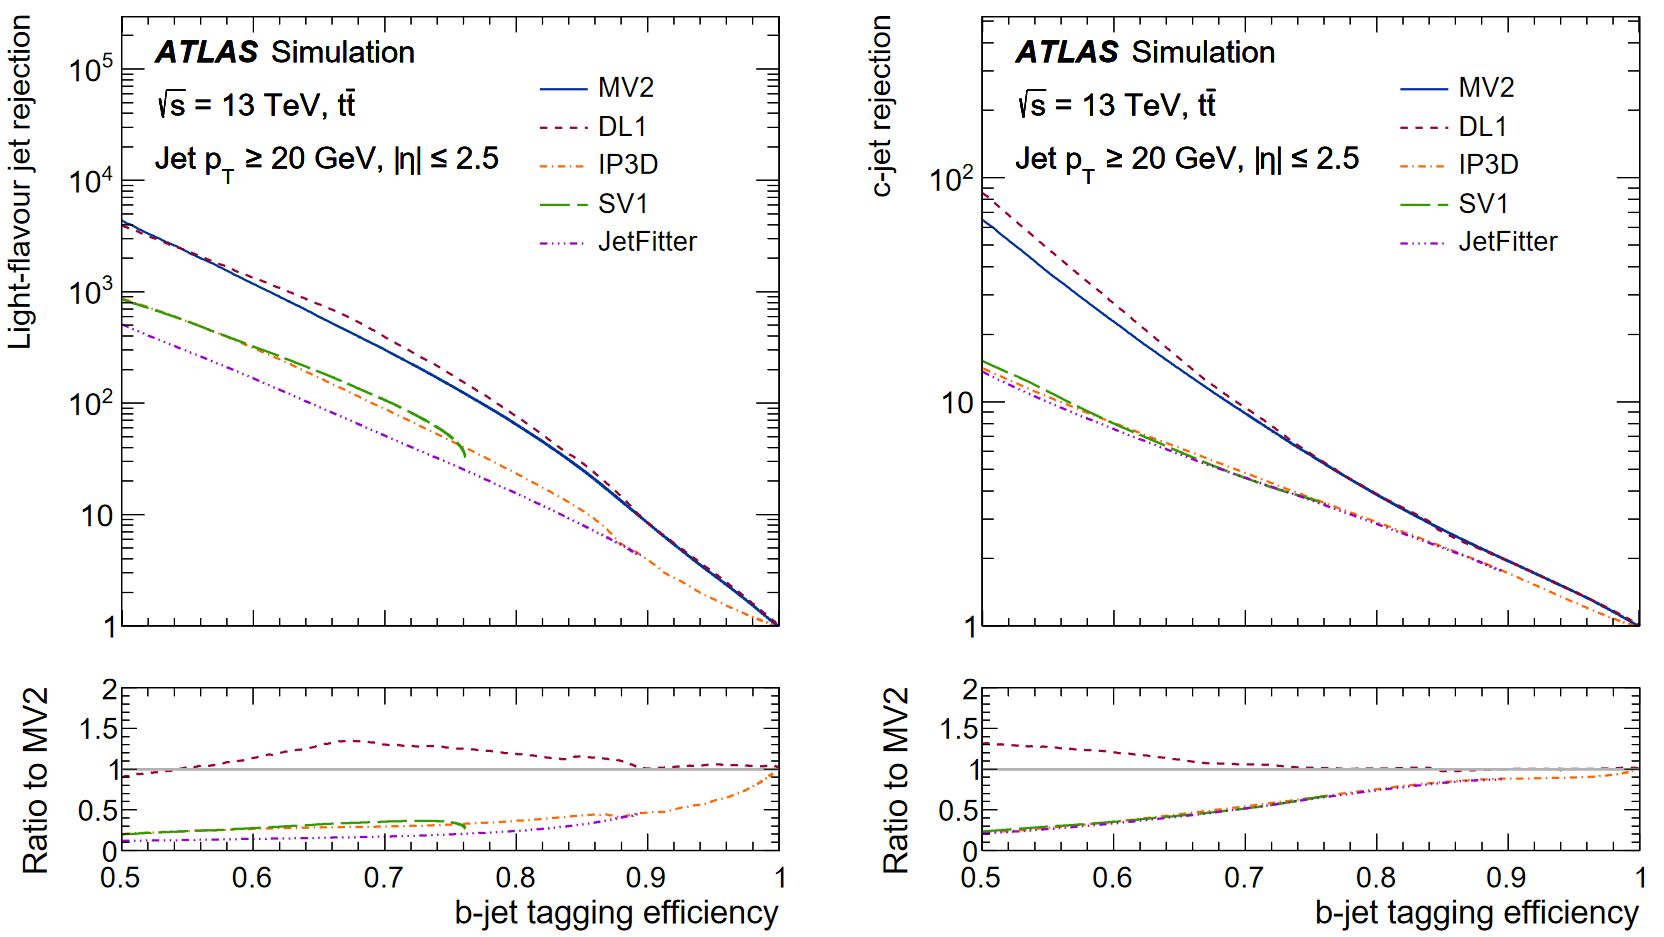
\includegraphics[width=1\textwidth]{FTAG_plots/b-tagging-perfermance.png}
	\caption{The light-flavour jet (left) and \cjet\ (right) rejections versus 
	the \bjet\ tagging efficiency for the IP3D, SV1, JetFitter, MV2 and
	DL1 b-tagging algorithms evaluated on the \ttbar\ events
	 \cite{FTAG-2018-01}.}\label{fig:b-tagging-performance}
\end{figure}


\begin{figure}[!h]
	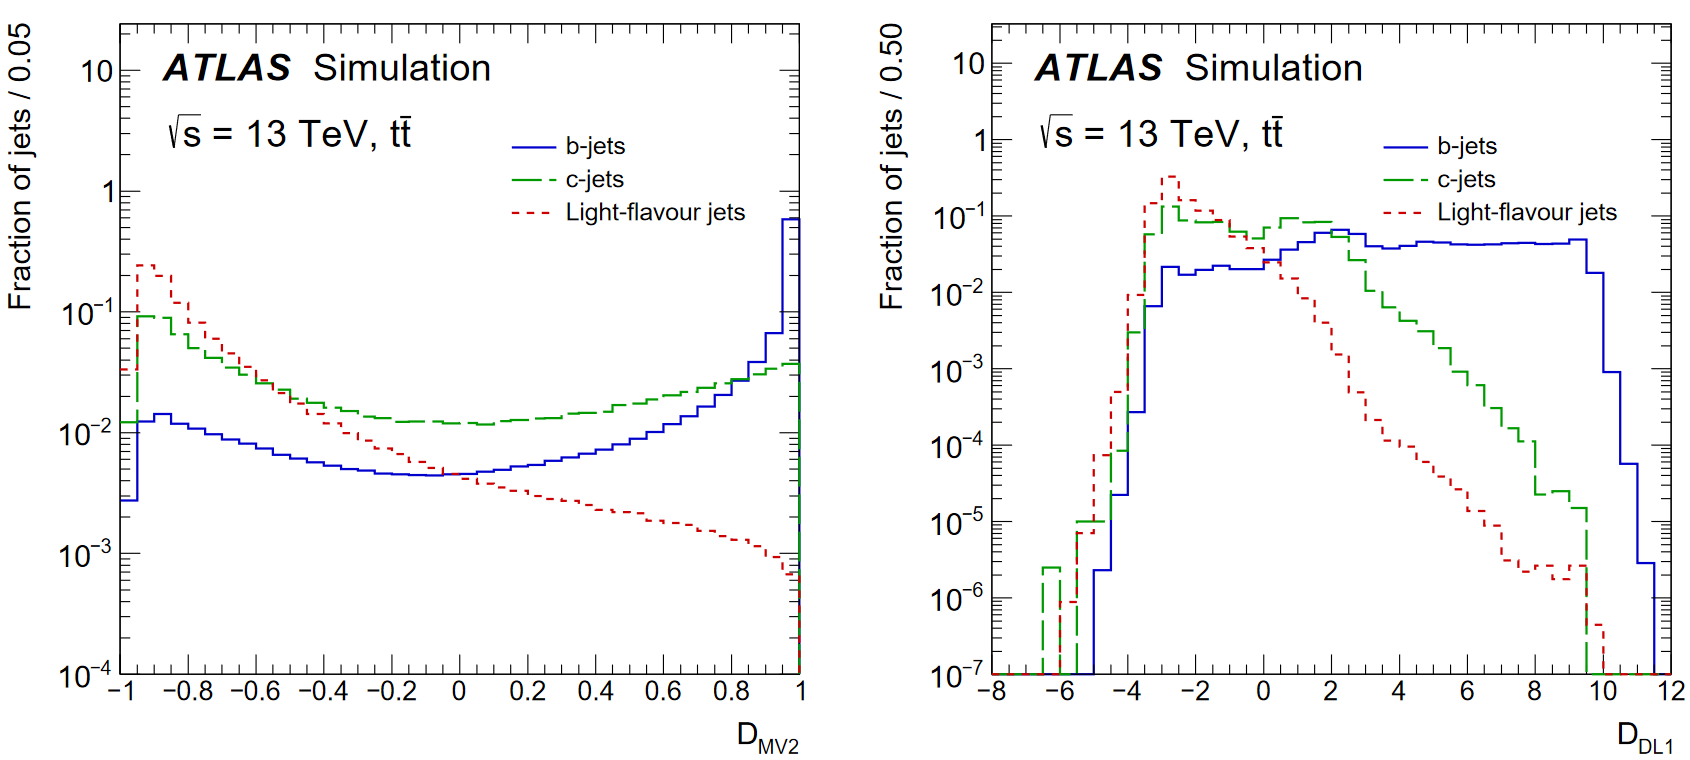
\includegraphics[width=1\textwidth]{FTAG_plots/b-tagging-score.png}
	\caption{The fraction of light-flavour jets and \cjets\ versus 
	the \bjets\ in the MV2 (left) and
	DL1 (right) b-tagging algorithms output distribution 
	evaluated on the \ttbar\ events
	 \cite{FTAG-2018-01}.}\label{fig:b-tagging-score}
\end{figure}


% The identification of the jets originating from the hadronization of heavy-flavour quarks is made possible by the distinctive properties of the heavy hadrons produced in the process. For instance, the large life time of $b$ quarks allows them to travel a measurable distance from the primary interaction point before to decay, giving rise to displaced tracks which can form secondary vertices. The ATLAS Collaboration developed several algorithms to identify (tag) the jets from $b$ quark hadronization based on the properties detailed above. 





\subsection{Missing transverse energy}
\subsection{Hadronically decaying $\tau$ lepton}


\section{Charm jet mis-tagging calibration}
%test
MC simulations are not able to model exactly the 
performance of the $b$-tagging algorithms in data. For this reason 
calibration is required, i.e.\ correcting MC to recover the data 
in terms of $b$-tagging efficiency, charm jet mis-tagging and 
light jet mis-tagging rates \cite{FTAG-2018-01}. The calibration is performed 
for all supported jet collections(TODO: refer back to the object definition chapter)
and working points, which are cuts in the \btagging\ 
algorithm output identifying the different tagging efficiencies 
and corresponding light jet and \cjet rejection rate.
In general, the efficiency is calculated with data and simulations, 
and scale factors are then calculated to match the efficiency extracted 
from simulations to the data.
\subsection{Calibration methods for \bjet\ and light jet}


In general, the efficiency is calculated with data and simulations, 
and scale factors are then calculated to recover the efficiency extracted 
from simulations to the data.
% The imperfect 
% description of the detector response and physics modelling effects 
% in Monte Carlo (MC) simulations necessitates the measurement of the 
% performance of the \btagging\ algorithms with collision data 
% \cite{PERF-2012-04,ATLAS-CONF-2018-045}. 
% The measurement of the \bjet\ tagging efficiency 
% of the high-level \btagging\ algorithms used in proton–proton (pp) 
% collision data recorded during Run 2 of the LHC at $\sqrt{s}$ = 13 TeV 
% is presented. 
% The corresponding measurements for \cjets\ and light-flavour 
% jets, used in the measurement of the \bjet\ tagging efficiency to correct 
% the simulation such that the overall tagging efficiency of \cjets\ and 
% light-flavour jets match that of the data, are described elsewhere 
% \cite{ATLAS-CONF-2018-006}, \cite{cjet}. 
The production of $t\bar{t}$ 
pairs at the LHC provides an abundant source of \bjets by virtue 
of the high cross-section and the $t \rightarrow Wb$ branching ratio 
being close to 100\%. A very pure sample of $t\bar{t}$ events can be 
selected by requiring that both $W$ bosons decay leptonically, 
referred to as di-leptonic $t\bar{t}$ decays in the following.
For the \bjet\ calibration, the performance of the $b$ tagging 
algorithms is evaluated in the simulation and the efficiency 
with which these algorithms identify jets containing $b$-hadrons 
is measured in collision data. The measurement uses a likelihood-based 
method in the di-leptonic $t\bar{t}$ sample, where
events with exactly 2 jets and 2 opposite-sign leptons are selected.  
The data \bjet\ efficiency is 
then extracted from a combined likelihood fit, and subsequently 
compared with that predicted by the simulation. Scale factors are 
then calculated to emulate the performance of the algorithms to the data \cite{FTAG-2018-01}.

For the light jet mis-tagging calibration, two methods are 
used to measure the mis-tagging rate from the data \cite{ATLAS-CONF-2018-006}. 
The first is the negative tag method, which uses a high statistics data sample enriched 
in light jets with the application of a modified algorithm which 
reverses some of the criteria used in the nominal identification 
algorithm.
The second is the adjusted Monte Carlo (adjusted-MC) method, which 
adjusts the characteristic track observables in the simulation 
to im the data, and then compares the adjusted simulation to the 
"standard" simulation. The scale factors are then calculated using 
the these two methods. The scale factors of the two different methods 
are in good agreement within the systematic uncertainties. 
%The aim of this calibration is to calibrate \bjets that have been mis-tagged as light jets of \btagging\ algorithm. As the $b$-tagging algorithm is very efficient in rejecting light jets, the light jet fraction is enriched via "flipped" taggers, which negates the sign of track IP parameters before $b$-tagging\cite{ATLAS-CONF-2018-006}. The calibrations of the standard and the 'flipped' tagger are assumed to be equal. The calibration is extracted using the leading $p_T$ jet of Z+jets events using a 2D fit. TODO: cite the light jet tagging Int note
%light jet fractions in the $b$-like region are too low,  The Z + jets events are then selected, the secondary vertex mass is fitted to obtain flavour fractions and perform a likelihood fit to extract light jet mistag rate.



\subsection{Calibration method for charm jet}
\label{sec:Calibration method for charm jet}

It is worth mentioning that the author's qualification task to become an ATLAS author is to 
calibrate the rate of a charm jet being mis-identified as a \bjet\, which is a part 
of the calibration of the $b$-tagging algorithm.
During the task the calibration range has been extended down to 20 GeV (previously 25 GeV) in
jet \pt\ and a new selection category has been developed 
to increase the data statistics of the scale factors in the 
high-$p_T$ ($p_T^{jet}$ > 70~GeV) region.
The calibration is performed on the PFlow jets and the VR-Track jets (TODO: refer back to definition in Object reconstruction section). 

As determined by the CKM matrix \cite{CKM1,CKM2}, the $W$ boson decays dominantly to 
a pair of light quarks ($u$ quark and $d$ quark) or to
a $s$ quark and a \cquark. The $W$ boson decays very rarely to pairs containing a \bquark. 
More specifically, the branching ratio of a $W$ boson decays to a $u$ quark and $d$ quark pair or 
a $s$ quark and $c$ quark pair is 33.1\%, and to pairs containing a $b$ quark is only 0.057\% \cite{PDG}. 
Therefore, $b$-tagged jets from the $W$ decay are most likely 
to be mis-tagged \cjets or light jets. 

Furthermore, given the ratio between the DL1 light jet rejection and the corresponding charm jet rejection 
ranges from 10 to 40 (Figure~\ref{fig:b-tagging-performance}), the 
\cjet\ is much more likely to be mis-tagged than the light jet. 
This allows for a source of mis-tagged \cjets to be obtained in the \ttbar\ events, 
requiring that one $W$ boson decays leptonically and the other decay hadronically 
(referred to as semi-leptonic $t\bar{t}$ decay in the following),
where the $b$-tagged jets from the $W$ decay are candidates of mis-tagged \cjets.
Requiring a $W$ boson decaying leptonically 
reduces the number of combinations of jets of different flavour, 
and allows triggering with the lepton.

The events kinematics are shown by the diagram in 
Figure \ref{fig:feynman}, where the \ttbar\ pair decays to a 
$b$ and a $\bar{b}$ quark, circled in red. One of the $W$ bosons, 
circled in blue, decays hadronically to quarks, 
and the other $W$ boson decays leptonically to either 
an electron or a muon and the corresponding neutrinos, 
circled in green and purple, respectively. 
The lepton in the final state is used for triggering.
The following notation will be used: the jets that are
the decay products of the $W$ boson are referred to as
$W$ jets and the remaining two jets are referred to as top-jets.

\begin{figure}[H]
\centering
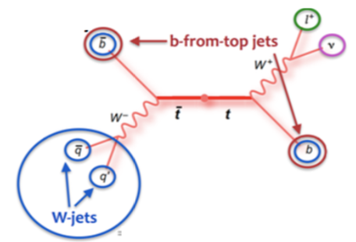
\includegraphics[width=.45\textwidth]{FTAG_plots/feynman.png}
\caption{Feynman diagram of the semi-leptonic $t\bar{t}$ events.}
\label{fig:feynman}
\end{figure}

%As Shown in Fig \ref{fig:feynman}, the calibration uses the semi-leptonic $t\bar{t}$ events, which one $W$ boson from top decays leptonically to a charged lepton and neutrino and one $W$ decays hadronically and dominantly to a charm and a strange quark, among other pairs.

A kinematic likelihood technique, referred to as 
KLFitter \cite{ERDMANN201418}, is used to assign jets to the proper $t\bar{t}$ decay product 
(more details in Section \ref{KLFitter}). 
The following notation will be used: the jets that are
assigned as the decay products of the $W$ boson are referred to as
$W$ jets and the remaining two jets are referred to as top jets.


The charm jet efficiency is defined as the ratio of events with either of the 
\wjet\ is tagged. The efficiency is evaluated in four \pt\ intervals, with 
boundaries of 20, 40, 65, 140 and 250 GeV for the PFlow jets and 15, 20, 40, 140 GeV
for the VR-Track jets; and for four tagging intervals with the boundaries of 85\%, 77\%,
70\% and 60\%. 

The choice of the bin boundaries ensures enough statistics for each bin and 
hence relatively flat statistical uncertainty, 
given the underlying charm-jet \pt\ spectrum as shown in Figure \ref{fig:kinematic_distributions_combined}.
The boundaries for the VR-Track jets are lower than for PFlow jets, 
since the track jets miss the neutral particles the
reconstructed energy is significantly below the true jet energy.

The main method described in the chapter is for the "fixed-cut" calibration
where the efficiency is defined as the fraction of \bjets passing the tagger.
Jets are said to be tagged (untagged) at particular working point
if they have DL1r scores greater (less) than the DL1r score of that working point.
The events with both \wjet\ are discarded to simplfiy the fit described in the following.

To extract the scale factors of the charm jet mis-tagging, a fit is performed by minimising 
the $\chi^2$ defined as:
\begin{eqnarray*}
\chi^2 = \sum_{t=1}^4 \sum_{i=1}^4  \sum_{j=1}^4 (N^{t}_{\mathrm{data}}(i,j)- p(i,j) [c^{t}(i)N^{t}_{C}(i,j)+N^{t}_{J}(i,j)+\sum_k  c^{4}(k) N^{t}_{X}(i,j,k)])^2/N^{t}_{\mathrm{data}}(i,j)
\end{eqnarray*}
\begin{eqnarray}
 +  \sum_{i=1}^4 \sum_{j=i}^4 [N^{\mathrm{untag}}_{\mathrm{data}}(i,j)-p(i,j)N^{\mathrm{untag}}_{\mathrm{MC}}(i,j)]^2/N^{\mathrm{untag}}_{\mathrm{data}}(i,j).
\label{eqn:chi2}
\end{eqnarray}
The $c^{t}(i)$ is the main floating parameter in the fit, which is the charm jet 
mis-tagging scale factor at working point $t$ of \pt\ bin labelled $i$. 
The other main floating parameter is $p(i,j)$ that is the normalisation factor scaling the MC to
data. 
The $N^{t}_{\mathrm{data}}(i,j)$ is the number of data events with a tagged \wjet\ in the \pt\ bin labelled i
and the other (untagged) \wjet\ in the \pt\ bin labelled j. Similarly the $N^{t}_{C}(i,j)$ is the number of MC events 
with a tagged \wjet\, while the tagged \wjet\ is indeed a \cjet\, which can be seen as "signal". 
In contrast the $N^{t}_{J}(i,j)$ is the number of events with neither the tagged \wjet\ nor the top jets 
are \cjets\; and the $N^{t}_{X}(i,j,k)$ is the number of events with one of the top jets is a \cjet\. 
These two types of events can be seen as "background". The later case is slightly more complicated, as the 
\cjet\ lies in a different \pt\ bin to the tagged jet, denoted as $k$, and it only depends on the 
$c^4(k)$ (which is the scale factor of the 4th working point i.e. 60\% ) as the top jets
are tagged at 60\% working point. 
The calibration is then given as the scale factors of the four working points 
in bins of \pt\ defined in the above text. 

% The charm-jet efficiency of the MC can be extracted from the truth information which indicates the 
% true nature of the $W$ jets. The \cjet\ efficiency of the MC is defined as the probability a true \cjet\ 
% is tagged by the \btagging\ algorithm in bins of jet \pt. 
% The charm-jet efficiency of the data is extracted by applying a combinatorial likelihood fit to $W$ jets, 
% where the main floating parameter are the \cjet\ efficiency
% in a given \pt\ bin and the ratio of data over total MC. 
% The calibration is given as scale factors in bins of \pt\ for 4 fixed-cut working points (WP) 
% that scale the simulation shape to reproduce that of the data, where the
% scale factors are calculated as the ratio of the data charm-jet efficiency over 
% the MC charm-jet efficiency. The calibration is performed for 4 \pt\ bins  
% (20, 40, 65, 140, 250) for the PFLow jets and (10, 20, 40, 65, 140) for the VR-Track jets
% in units of GeV. 







\subsection{Data and Monte Carlo samples}
%%%%%%%%%%%%%%%%%%%%%%%%%%%%%%%%%%%%%%%%%%%%%%%

\label{sec:samples}
TODO: remove the overlap between this section and the Data MC chapter in the thesis
Dedicated MC are used to model SM processes. 
%%%%%%%%%%%%%%%%%%%%%%%%%%%%%%%%%%%%%%%%%%%%%%%
The data analysed in this study correspond to 139~fb$^{-1}$~\cite{DAPR-2010-01,DAPR-2011-01,DAPR-2013-01,LUCID2}, 
of \(pp\) collision data collected by the ATLAS detector between 2015 and 2018
with a centre-of-mass energy of 13~\TeV. 
The data sample was collected using a set of single-muon~\cite{Aad:2020uyd} 
and single-electron triggers~\cite{TRIG-2018-05}. The single-muon triggers 
had \pt\ thresholds in the range 20--26~\GeV\ for 
isolated muons and 50~\GeV\ for muons without any isolation requirement. 
The single-electron triggers employed a range of \pt\ thresholds 
varying between 24--300~\GeV\ 
and a combination of quality and isolation requirements depending on the 
data-taking period and the \pt\ threshold.
%The uncertainty in the combined 2015--2018
%integrated luminosity is 1.7\%~\cite{ATLAS-CONF-2019-021}, obtained
%using the LUCID-2 detector~\cite{LUCID2} for the primary luminosity
%measurements. 
All detector subsystems were required to be operational
during data taking and to fulfil data quality requirements.  

% The $t\bar{t}$ samples and the single top-quark in the Wt 
% and s-channel samples are generated with the {\tt Powheg-Box} v2 \cite{powheg} 
% generator. Electroweak t-channel single top-quark events are generated 
% using the {\tt Powheg-Box} v1 generator. The parton shower, fragmentation, 
% and the underlying event are simulated using {\tt Pythia} 6.428\cite{pythia} 
% with the CTEQ6L1 PDF sets and the corresponding Perugia 2012 tune (P2012)\cite{perugia}. 
% The top-quark mass is set to 172.5 GeV. The {\tt EvtGen} v1.2.0 program \cite{evtgen} 
% is used to model the properties of the bottom and charm hadron decays. 
% The $t\bar{t}$ production cross-section is calculated at NNLO+NNLL 
% (next-to-next-to-leading-logarithm)\cite{NNLO}. For single-top processes, 
% the generator NLO cross-sections are used. Events containing $W$ or $Z$ 
% bosons with associated jets are simulated using {\tt Sherpa} 2.2.1\cite{sherpa}. 
% All $W$/$Z$+jets events are normalised to the predicted cross-sections using 
% NNLO calculations. All samples are passed through the full GEANT4\cite{GEANT4} 
% simulation of the ATLAS detector and are reconstructed with the same software as used for data.



All samples were 
produced using the ATLAS simulation infrastructure~\cite{SOFT-2010-01}
and $\GEANT4$~\cite{Agostinelli:2002hh}. A subset of samples use a faster 
simulation based on a parameterisation of the calorimeter response and 
$\GEANT4$ for the other detector systems~\cite{SOFT-2010-01}. %\cite{ATL-PHYS-PUB-2010-013}.
The simulated events are reconstructed with the same algorithms as
used for data, and contain a realistic modelling of pile-up
interactions. The pile-up profiles in the simulation match those of each dataset
between 2015 and 2018, and are obtained by overlaying minimum-bias events,
simulated using the soft QCD processes of
{\PYTHIA}~8~\cite{Sjostrand:2014zea} using the NNPDF2.3LO set of
PDFs~\cite{Ball:2012cx} and a set of tuned
parameters called the A3 tune~\cite{ATL-PHYS-PUB-2016-017}.

The events that are used in this study originate mostly due to 
\ttbar\ production. This process is modelled using the
\powhegbox~v2~\cite{Frixione:2007nw,Nason:2004rx,Frixione:2007vw,Alioli:2010xd}
generator at NLO with the \nnpdfnlo % ~\cite{Ball:2014uwa}
parton distribution function (PDF) set
and the \hdamp\ parameter\footnote{The
  \hdamp\ parameter is a resummation damping factor and one of the
  parameters that controls the matching of \powheg matrix elements to
  the parton shower and thus effectively regulates the
  high-\pt\ radiation against which the \ttbar\ system recoils.} set
to 1.5~\mtop~\cite{ATL-PHYS-PUB-2016-020}.  The events were interfaced
to {\PYTHIA}~8.230 to model the parton shower,
hadronisation, and underlying event, with parameters set according
to the A14 tune and using the \nnpdftwo set of PDFs.
The decays of bottom and charm hadrons were performed by \evtgen~v1.6.0~\cite{EvtGen}.
 The simulated \ttbar\
events are split according to the origin of $W$ jets. The notation
``\ttbar, ll'' denotes that both $W$ jets are light flavour jets.
Similarly, ``\ttbar, cl'' (``\ttbar, bl'') 
indicates that one of the $W$ jets is a \cjet\ (\bjet)
whereas the other is a light flavour jet. $W$ jets with origin
other than what is discussed above fall into the 
category denoted by ``\ttbar, other''. This category includes
events in which at least one of the $W$ jets comes from a
hadronically decaying $\tau$-lepton. 

%%% single top
In addition to \ttbar\ production, there are some minor backgrounds
that contribute to the final event sample that is used for the calibration.
These backgrounds consist mostly of single-top and diboson production, 
the production of \ttbar\ in association with a vector boson
and the production of a vector boson in association with jets.
The details
of the modeling of these samples are given in the following.

Single-top $s$-channel production is modelled using the \powhegbox~v2 % \cite{Alioli:2009je,Nason:2004rx,Frixione:2007vw,Alioli:2010xd}
generator at NLO in QCD in the five-flavour scheme with the \nnpdfnlo~\cite{Ball:2014uwa} parton distribution function~(PDF) set.
%The events are interfaced with \pythia.230 % ~\cite{Sjostrand:2014zea} 
%using the A14 tune % ~\cite{ATL-PHYS-PUB-2014-021}
%and the \nnpdftwo PDF set.
%
The associated production of top quarks with $W$ bosons ($tW$) is
modelled using the
\powhegbox~v2~\cite{Re:2010bp,Nason:2004rx,Frixione:2007vw,Alioli:2010xd}
generator at NLO in QCD using the five-flavour scheme and the
\nnpdfnlo set of PDFs~\cite{Ball:2014uwa}.
The diagram removal scheme~\cite{Frixione:2008yi} is used to
remove interference and overlap with \ttbar\ production. 
The events for both single-top $s$-channel and $tW$ production 
are interfaced to \pythia.230%~\cite{Sjostrand:2014zea} 
using the A14 tune%~\cite{ATL-PHYS-PUB-2014-021} 
and the \nnpdftwo set of PDFs. %~\cite{Ball:2012cx}.

The production of $Z+$jets and $W$+jets is simulated with the
\sherpa~v2.2.1~\cite{Bothmann:2019yzt}
generator using next-to-leading order (NLO) matrix elements (ME) for up to two partons, and leading order (LO) matrix elements
for up to four partons calculated with the Comix~\cite{Gleisberg:2008fv}
and \openloops~\cite{Buccioni:2019sur,Cascioli:2011va,Denner:2016kdg} libraries. They
are matched with the \sherpa parton shower~\cite{Schumann:2007mg} using the MEPS@NLO
prescription~\cite{Hoeche:2011fd,Hoeche:2012yf,Catani:2001cc,Hoeche:2009rj}
using the set of tuned parameters developed by the \sherpa authors.
The \nnpdfnnlo set of PDFs~\cite{Ball:2014uwa} is used and the samples
are normalised to a next-to-next-to-leading order (NNLO)
prediction~\cite{Anastasiou:2003ds}.

Samples of diboson final states ($VV$) are simulated with the
\sherpa~v2.2.1 or v2.2.2~\cite{Bothmann:2019yzt} generator depending on the process,
%~\footnote{This is an admixture of 2.2.1 and above versions, so the version should be kept generic to avoid confusions. As an alternative, the sentence can be modified indicating that samples are simulated with the \sherpa~v2.2.1 or v2.2.2 depending on the process.} 
including off-shell effects and Higgs-boson contributions, where appropriate.
Fully leptonic final states and semileptonic final states, where one boson
decays leptonically and the other hadronically, are generated using
matrix elements at NLO accuracy in QCD for up to one additional parton
and at LO accuracy for up to three additional parton
emissions. Samples for the loop-induced processes $gg \to VV$ are
generated using LO-accurate matrix elements for up to one
additional parton emission for both cases of fully leptonic and
semileptonic final states. The matrix element calculations are matched
and merged with the \sherpa parton shower based on Catani-Seymour
dipole factorisation~\cite{Gleisberg:2008fv,Schumann:2007mg} using the MEPS@NLO
prescription~\cite{Hoeche:2011fd,Hoeche:2012yf,Catani:2001cc,Hoeche:2009rj}.
The virtual QCD correction are provided by the
\openloops library~\cite{Buccioni:2019sur,Cascioli:2011va,Denner:2016kdg}. The
\nnpdfnnlo set of PDFs is used, %~\cite{Ball:2014uwa}, 
along with the dedicated set of tuned parton-shower parameters developed by the
\sherpa authors.

The production of \ttbar\ in assosiation with a vector boson 
is modelled using the
\mgamc~v2.3.3~\cite{Alwall:2014hca} generator at NLO with the
\nnpdfnlo~\cite{Ball:2014uwa} parton distribution function~(PDF).
The events are interfaced to \pythia.210~\cite{Sjostrand:2014zea}~
using the A14 tune~\cite{ATL-PHYS-PUB-2014-021} and the
\nnpdftwo~\cite{Ball:2014uwa} PDF set. The decays of bottom and charm
hadrons are simulated using the \evtgen\ v1.2.0 program~\cite{Lange:2001uf}.



\subsection{Kinematic Likelihood Fitter}
\label{KLFitter}
% Top quarks decay to a $W$ boson and a bottom quark in nearly 100\% of all 
% cases. Consequently, the final state of a top-quark pair is characterised by 
% the decay products of the two $W$ bosons. 
% %If one of the $W$ bosons decays into a charged lepton and a neutrino while the other one decays into a pair of quarks, the decay mode is referred to as the single-lepton, or semi-leptonic decay mode. 
% The fraction of top-quark pairs decaying either in the 
% single-electron or single-muon decay mode 
% is about 30\%. The corresponding event signature is defined 
% by exactly one electron or muon, four jets out of which 
% two contain a $b$-hadron, and a large amount of missing transverse momentum 
% due to the un-detected neutrino. The Kinematic Likelihood Fitter\cite{ERDMANN201418}, 
% is a reconstruction technique developed to reconstruct $t\bar{t}$ decays, 
% which exploits the above decay topology of the top quark in the 
% semi-leptonic channel in order to properly associate jets to the 
% quarks in the final state of the decay process. In the semi-leptonic 
% decay of the $t\bar{t}$ system, the resulting tree level situation 
% contains two $b$ quarks from the top quark decays, and two light or 
% charm quarks from the $W$ boson decay (Figure \ref{fig:feynman}). 
% A likelihood is used to properly assign these four jets to the true 
% decay quarks. The leading order scenario is assumed, giving rise to four jets 
% in the final $t\bar{t}$ decay topology, two of which are \bjets. Three 
% of the jets in the decay are associated to the hadronic top decay, 
% whereas a final fourth jet along with the charged lepton and 
% neutrino build the leptonic top\cite{cjet}.
The four-vectors of the four highest \pt\ jets, the lepton and the
event \MET\ are used as inputs to a likelihood-based \ttbar\ event
reconstruction algorithm, which is described in more detail in
Ref.~\cite{ERDMANN201418}. This algorithm uses a likelihood function
to assign the four jets to the \ttbar\ decay topology. In particular,
the algorithm assigns one jet to be the \bjet\ from the leptonically
decaying top quark ($t\to Wb \to \ell \nu b$), another to the \bjet\
from the hadronically decaying top quark ($t\to Wb \to qq^\prime b$,
where $qq^\prime$ are the quarks in which the $W$ boson decays) and
the remaining two jets to the jets that come from the hadronic $W$
boson decay. The jet assignment does not use any \btagging\ information
to avoid bias.



\subsection{Maximising likelihood}
\label{maximise likelihood}
\begin{figure}[!h]
	\centering
	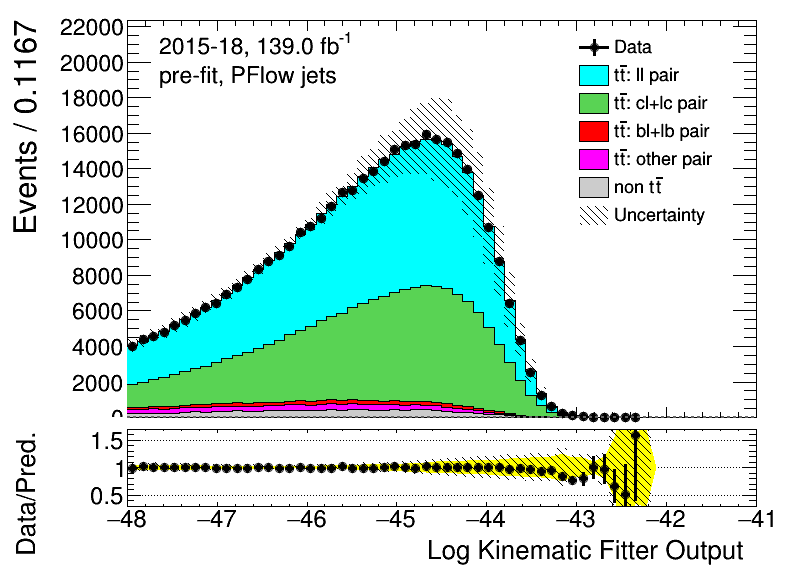
\includegraphics[width=0.45\textwidth]{FTAG_plots/pretagNoRwwithhighpTPFlowall/DataMC_h_LLR.png}
	\caption{Distribution of  the negative logarithm of the likelihood that
	is used to reconstruct the \ttbar\ decay.}
	\label{fig:llr}
\end{figure}

Taking only four jets in the event limits the total number of possible 
jet orderings (permutations) in the event. In the semi-leptonic channel, 
four jets can be permuted a total number of times equal to 4! = 24. 
However, the two $W$ jets are kinematically indistinguishable. 
This reduces the possible number of permutations to 12. 
%Furthermore, no $b$-tagging information is used 
%in the kinematic likelihood to limit the possible number of permutations
%as this would bias the result.
For every combination of jet ordering, 
the likelihood is maximised over 
its free parameters, the energy of the four jets, the lepton energy and 
the three components of the momentum of the neutrino, and provides a 
value based on how closely the kinematic information from the reconstructed 
objects for a specific jet ordering resembles the expected kinematic behaviour 
of the decay of a Standard Model semi-leptonic $t\bar{t}$ event. The likelihood 
therefore distinguishes the possible permutations on an event-by-event basis. 
The best permutation, given by the largest log-likelihood value, is adopted 
as the jet ordering for the event. 
An additional requirement of log-likelihood > -48 is 
placed on the output of the likelihood value for the chosen event permutation. 
An example of the distribution of log-likelihood of the best permutations 
is shown in Figure \ref{fig:llr}. 
In this figure, the data events are compared against the simulation.
The majority of the events come from \ttbar\ production. There is only
a very small fraction of events, which is denoted as ``non \ttbar''
on the figure, that come from other processes like $W$ or $Z$ production
in association with jets or single-top production.


\subsection{Event selection}
\label{Event selection}
 % The analysis uses the full available integrated luminosity collected with the ATLAS detector from the all years. This corresponds to a collected luminosity of 139 fb$^{-1}$. The event selection aims to select a sample enriched in $t\bar{t}$ events. The lowest un-prescaled single electron and single-muon triggers are used.
\subsubsection{Standard selection}
\label{standard selection}

\begin{table}[ht]
	\centering
	\small
	\setlength\tabcolsep{5pt} 
	\newcolumntype{C}{ @{}>{${}}c<{{}$}@{} }
	\begin{tabular}{|r *2{|rCr}| }
	\hline
	& \multicolumn{3}{|c|}{PFlow jets} & \multicolumn{3}{c|}{Track jets} \\
	\hline
	Data          &     227118       &   &              &   218351  &       &         \\  
	\ttbar\       &     235670       &\pm& 200          &   223770  &\pm& 180     \\
	Non \ttbar\   &     7610         &\pm& 120          &   7280    &\pm& 100    \\
	\hline
	Data/MC       &     0.934        &\pm& 0.002        &   0.945   &\pm& 0.002 \\
	\hline
	\end{tabular}
	\vspace{0.2cm}
	\caption{Standard selection: prefit comparison of the  number of events in data and in 
	simulation considering the PFlow jets and the VR-Track jets for 
	events with exactly 4 jets.}
	\label{tab:yields_standard}
\end{table}
\begin{figure}[H]
	\centering
	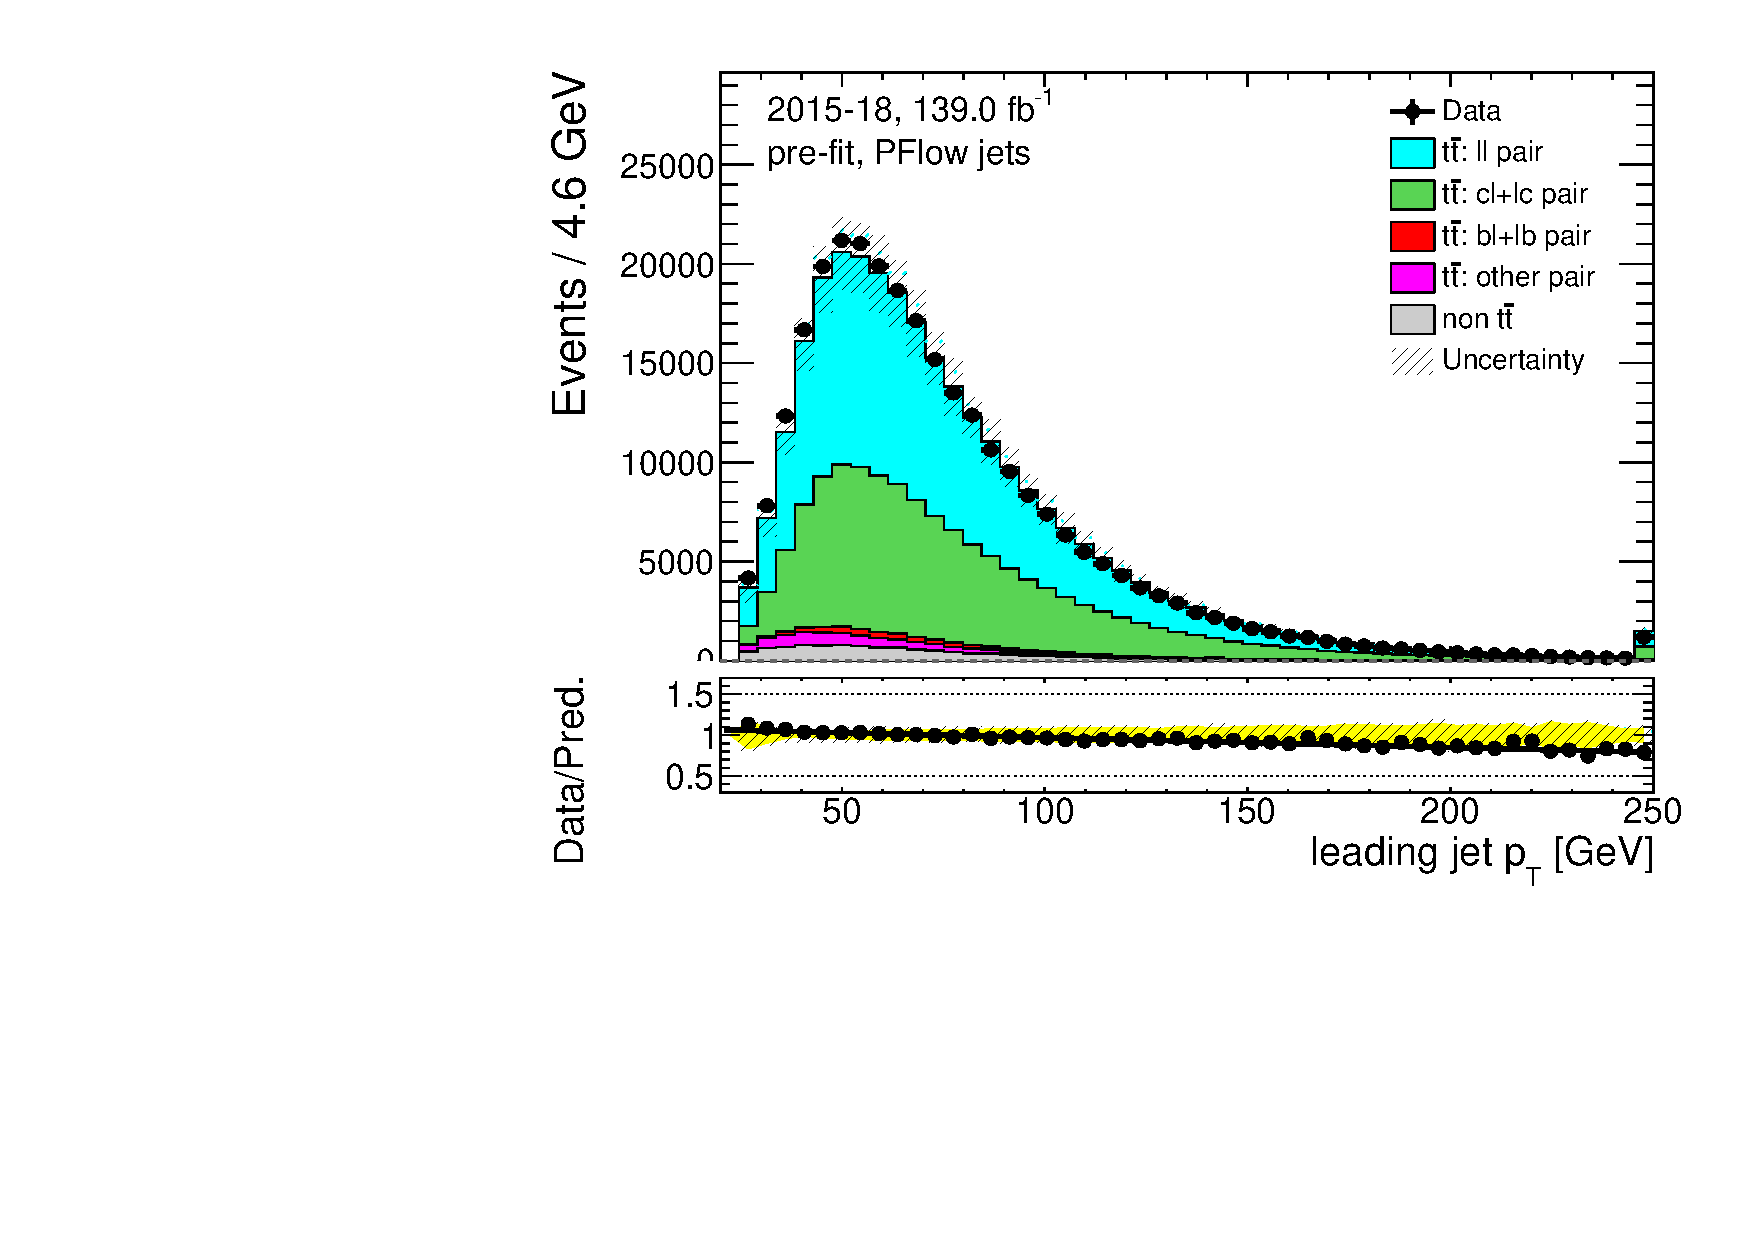
\includegraphics[width=0.45\textwidth]{FTAG_plots/pretagNoRwwithouthighpTPFlowall/DataMC_h_J0_pt.pdf}
	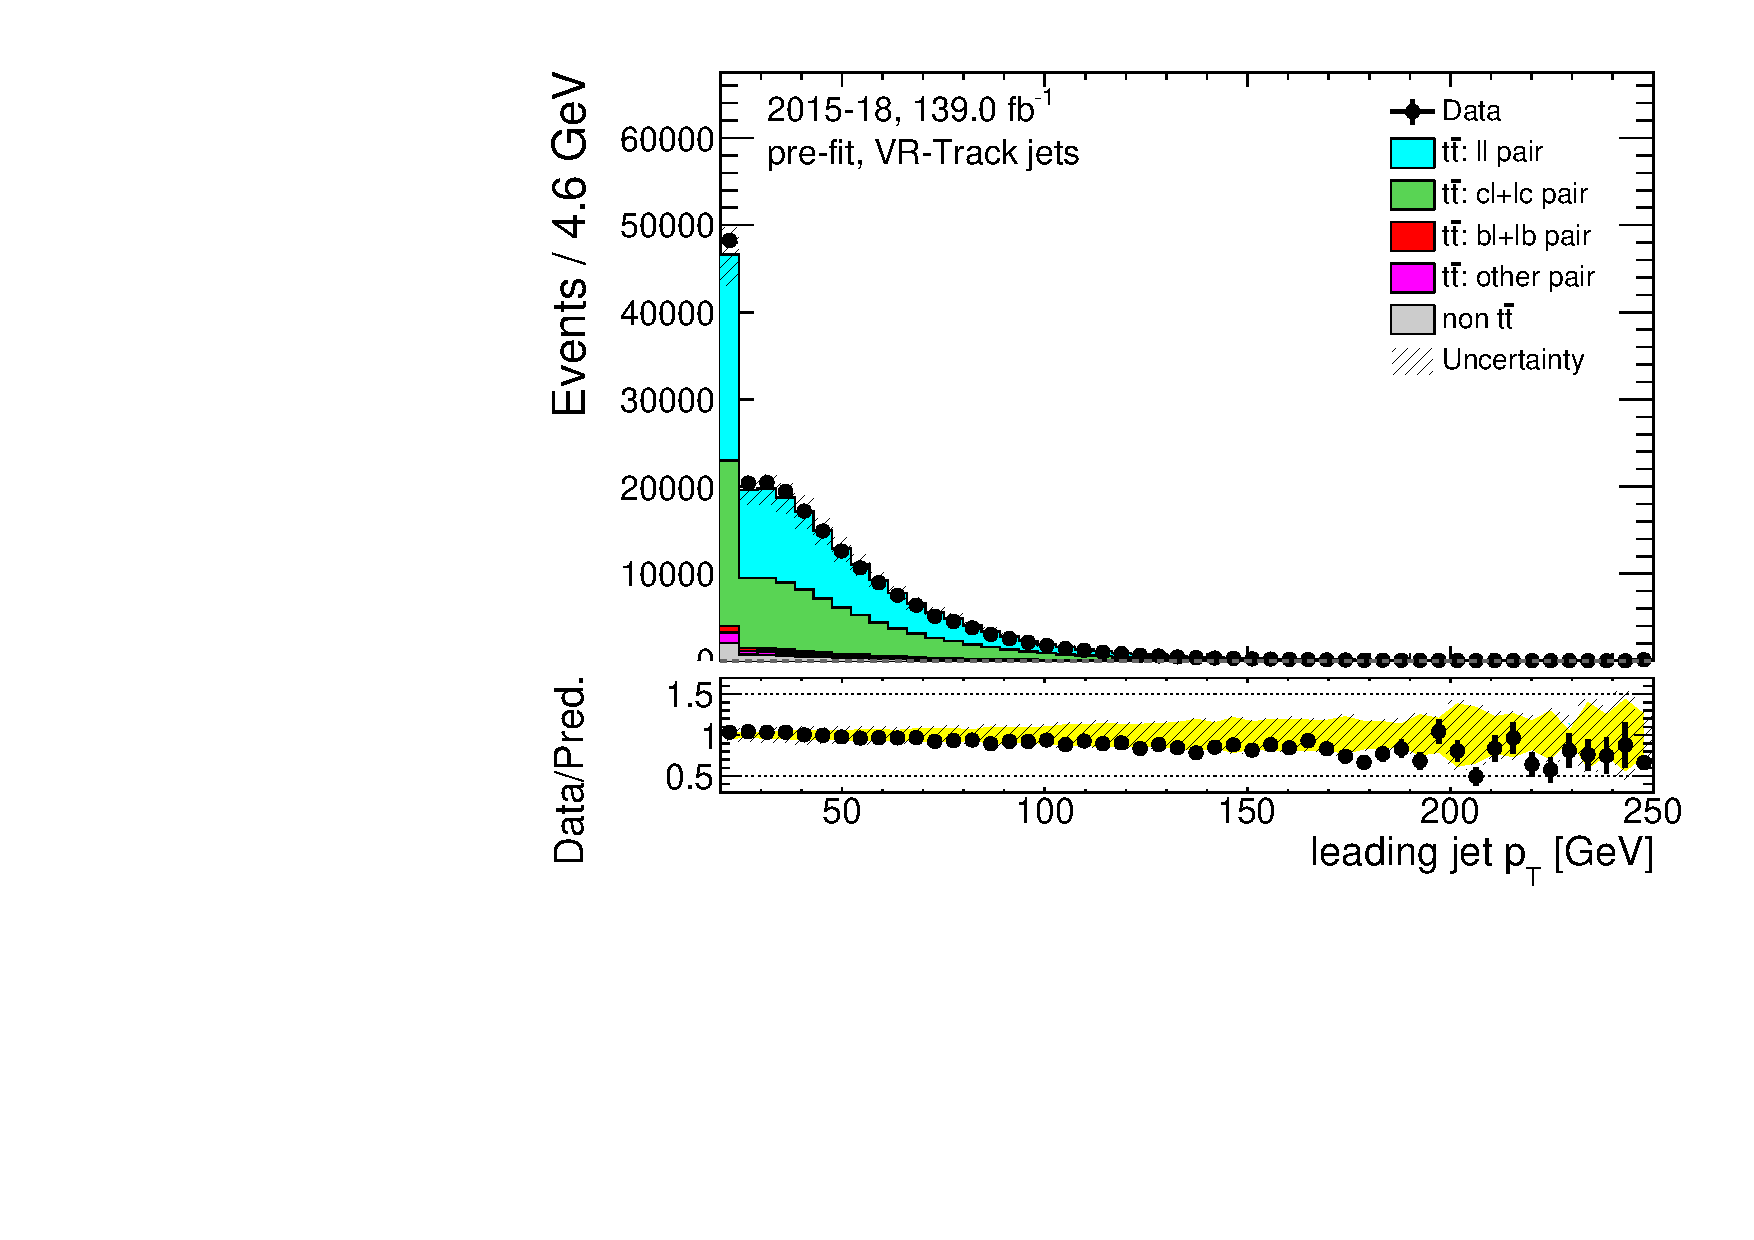
\includegraphics[width=0.45\textwidth]{FTAG_plots/pretagNoRwwithouthighpTVRJetsall/DataMC_h_J0_pttrackjet.pdf}\\
	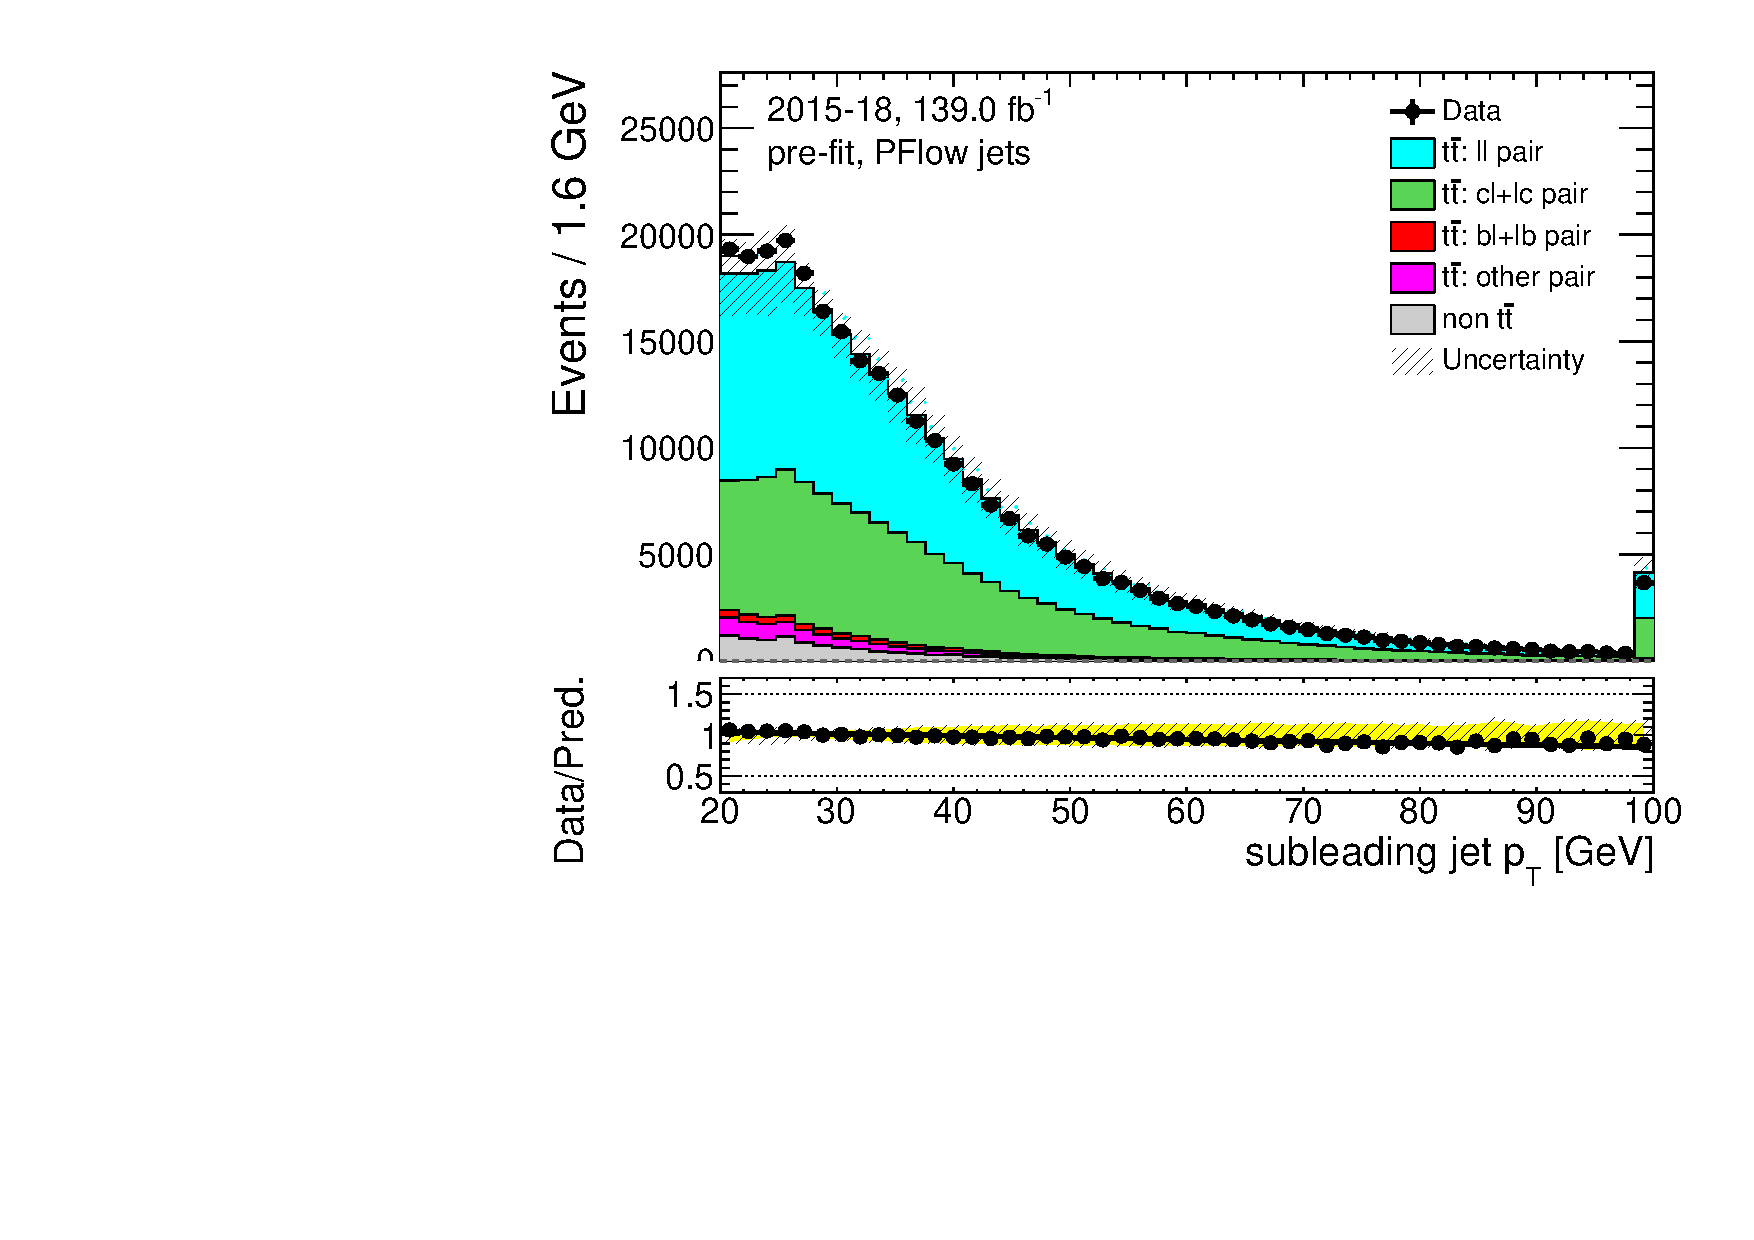
\includegraphics[width=0.45\textwidth]{FTAG_plots/pretagNoRwwithouthighpTPFlowall/DataMC_h_J1_pt.pdf}
	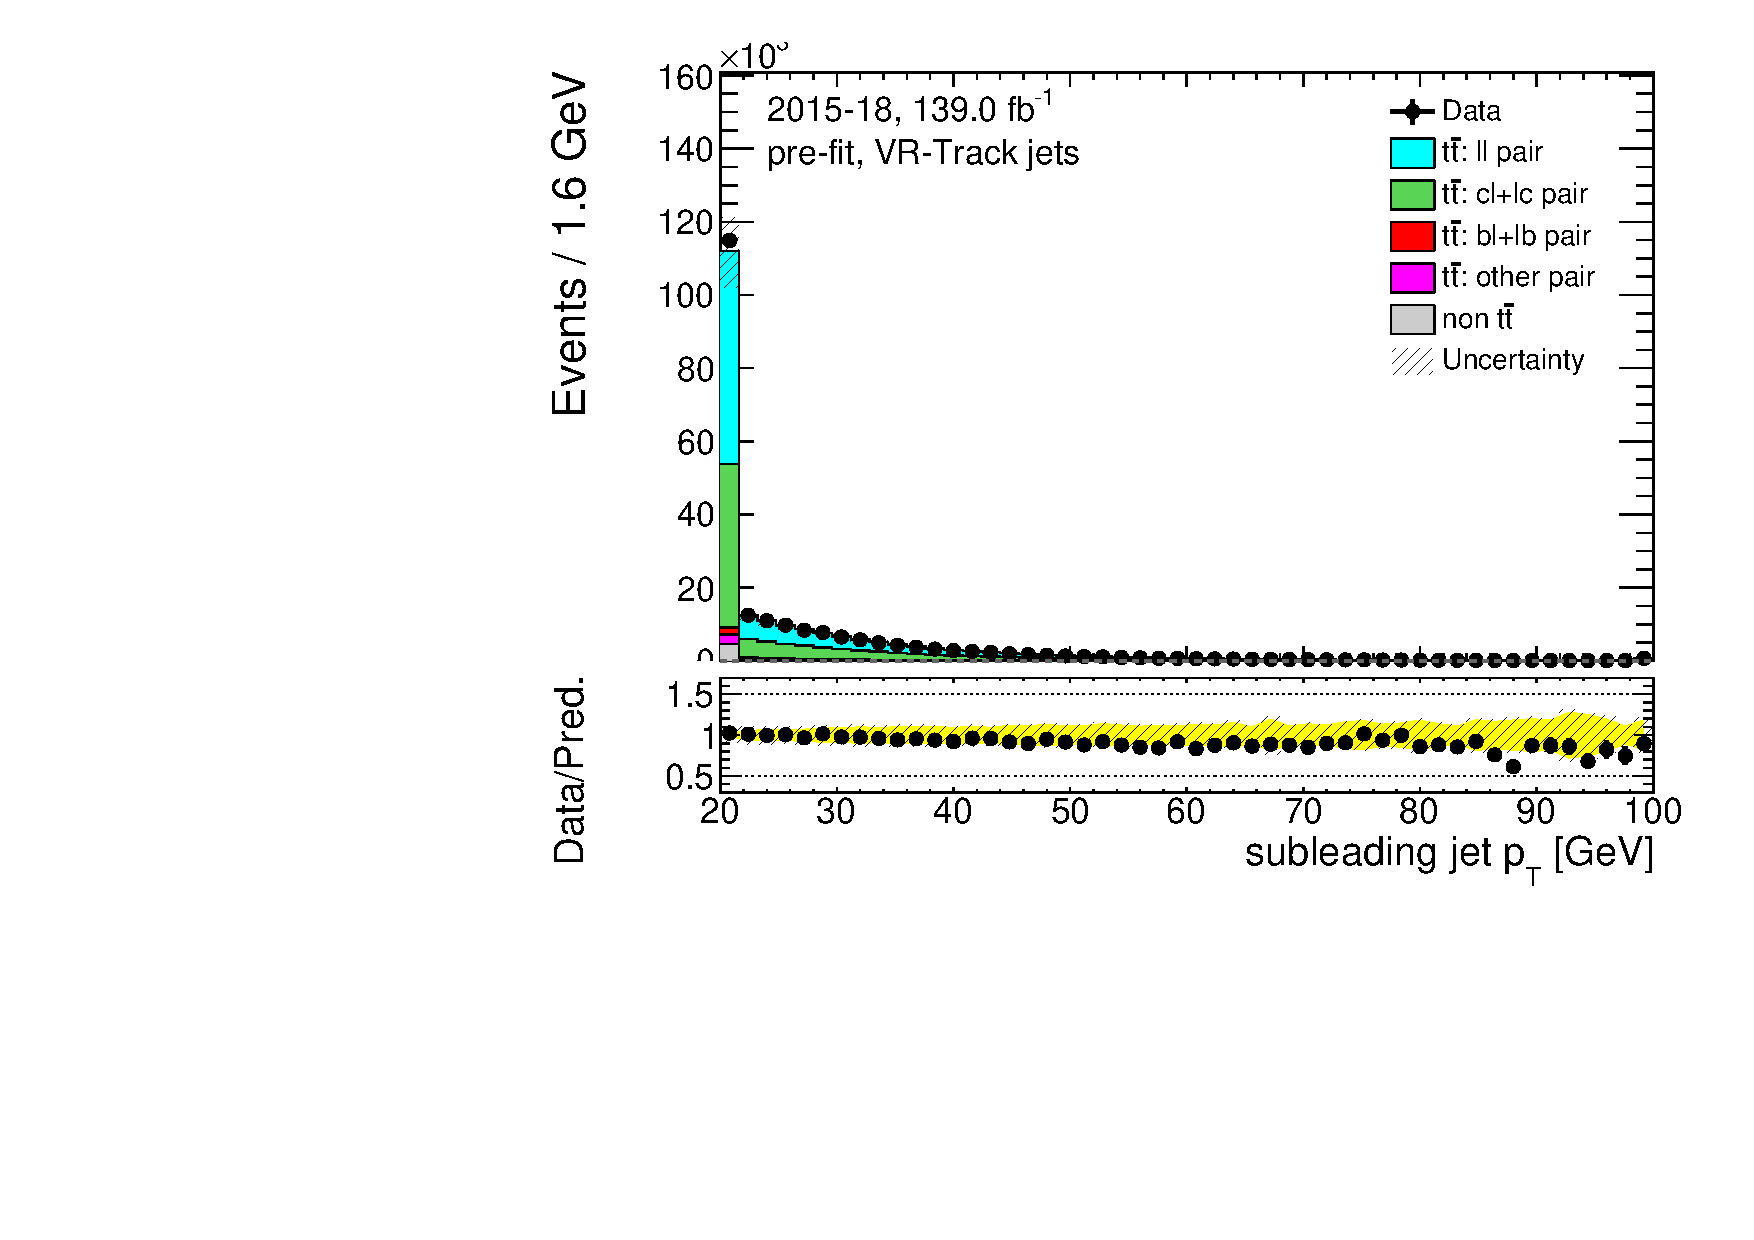
\includegraphics[width=0.45\textwidth]{FTAG_plots/pretagNoRwwithouthighpTVRJetsall/DataMC_h_J1_pttrackjet.pdf}\\
	\caption{Standard selection: data versus simulation of the leading and sub-leading $W$ jet \pt\ 
	for the PFlow jets in the left column and for VR-Track jets in the right column. 
	The leading jet and sub-leading jet refer to the highest \pt\ $W$ jet and the 
	second highest \pt\ jet, respectively. The 'non \ttbar' background 
	indicates background comes from non-\ttbar\ processes like $W$ or $Z$ production
	in association with jets or single-top production.
	The error in the table (and the following yields tables for
	different selection) is stats-only. }
	\label{fig:kinematic_distributions_standard}
\end{figure}

Events are required to contain exactly one trigger-matched 
lepton with $p_{T} > 27$~GeV and exactly four jets with 
$p_{T} > 25$~GeV. Leptons are required to have $p_{T}$ 
above 27 GeV in order to avoid the turn-on curve for the 
single lepton triggers. Events which contain an additional 
lepton with $p_T > 27$~GeV are rejected. 
The events are also required to have $\MET > 20$~GeV, which is 
assumed to be the result of the neutrino from the leptonically 
decaying $W$ boson. The transverse
mass $m_T$ between the lepton and the \MET, is
constrained as follows:
\[ m_T = \sqrt{2 p_T^\ell \MET (1-\cos\Delta\phi)} > 40~\GeV,\]
where $\Delta\phi = \phi(\MET)-\phi(\ell)$ is the azimuthal difference between
the lepton and \MET.
% Due to the requirement on jet $p_T$ and binning strategy, the calibration 
% result can be applied to jets with $p_{T}$ between 25 to 200 GeV. 
The yields of the data and the MC are given in Table \ref{tab:yields_standard}.
An example of the \pt\ distributions
before any tagging or fitting and 
after the standard selection is shown in Figure \ref{fig:kinematic_distributions_standard}. 
More plots can be found in Appendix \ref{sec:appendix_standard_selection}.
The yellow band in the lower pad shows the overall systematic uncertainties, combining the 
experimental uncertainties and the \ttbar\ modelling uncertainties, as described in 
Section \ref{sec:FTAG_systematics}. The data/MC ratio shows good agreement 
within the systematic uncertainties. 

\subsubsection{Low-\pt\ selection}
\label{sec:lowpT_selection}
The author has developed an othorgonal selection to 
extend the calibration in the low-$p_{T}$ region so that the calibration 
can be applied to PFlow jets with $20< \pt\ < 25$~GeV.
The \pt\ threshold of the VR-Track jets is $10$~GeV 
therefore the low-\pt\ selection is not needed. 
Instead of requiring events to 
have exactly 4 jets $\pt\ > 25$~GeV, events are required to have exactly 3 jets with $p_{T} > 25$~GeV 
and exactly 1 jet with $25$~GeV $> p_{T} > 20$~GeV. Other than that, 
all requirements for the selection are the same. 
This additional cut provides candidates for the PFlow $W$ jet that is used 
for calibration in the $20-25$~GeV region. 
The inclusive yields of the low-\pt\ selection 
of the data and the MC are given in Table \ref{tab:yields_lowpT}, and
the \pt\ distributions of the $W$ jets are shown in Figure \ref{fig:kinematic_distributions_lowpT}.
More plots of the kinematic distributions
are shown in Appendix \ref{sec:appendix_lowpT_selection}. 
Good agreement between MC and data 
is shown in these distributions, and the $p_{T}$ range of the sub-leading has gone down to 20 GeV. 


\begin{table}[ht]
	\centering
	\small
	\setlength\tabcolsep{5pt} 
	\newcolumntype{C}{ @{}>{${}}c<{{}$}@{} }
	\begin{tabular}{|r *1{|rCr}| }
	\hline
	& \multicolumn{3}{|c|}{PFlow jets} \\
	\hline
	Data          &     59987       &   &                      \\  
	\ttbar\       &     56530       &\pm&     90        		 \\
	Non \ttbar\   &     3340        &\pm&     60    		 \\
	\hline
	Data/MC       &     1.002       &\pm&  0.004      			 \\
	\hline
	\end{tabular}
	\vspace{0.2cm}
	\caption{Low-\pt\ selection: prefit comparison 
	of the number of events in data and MC 
	for the PFlow $W$ jets. Events are required to have 
	exactly 3 jets with $\pt\ > 25$~GeV 
	and one jet with $20 < \pt\ < 25$~GeV.}
	\label{tab:yields_lowpT}
\end{table}

\begin{figure}[H]
	\centering
	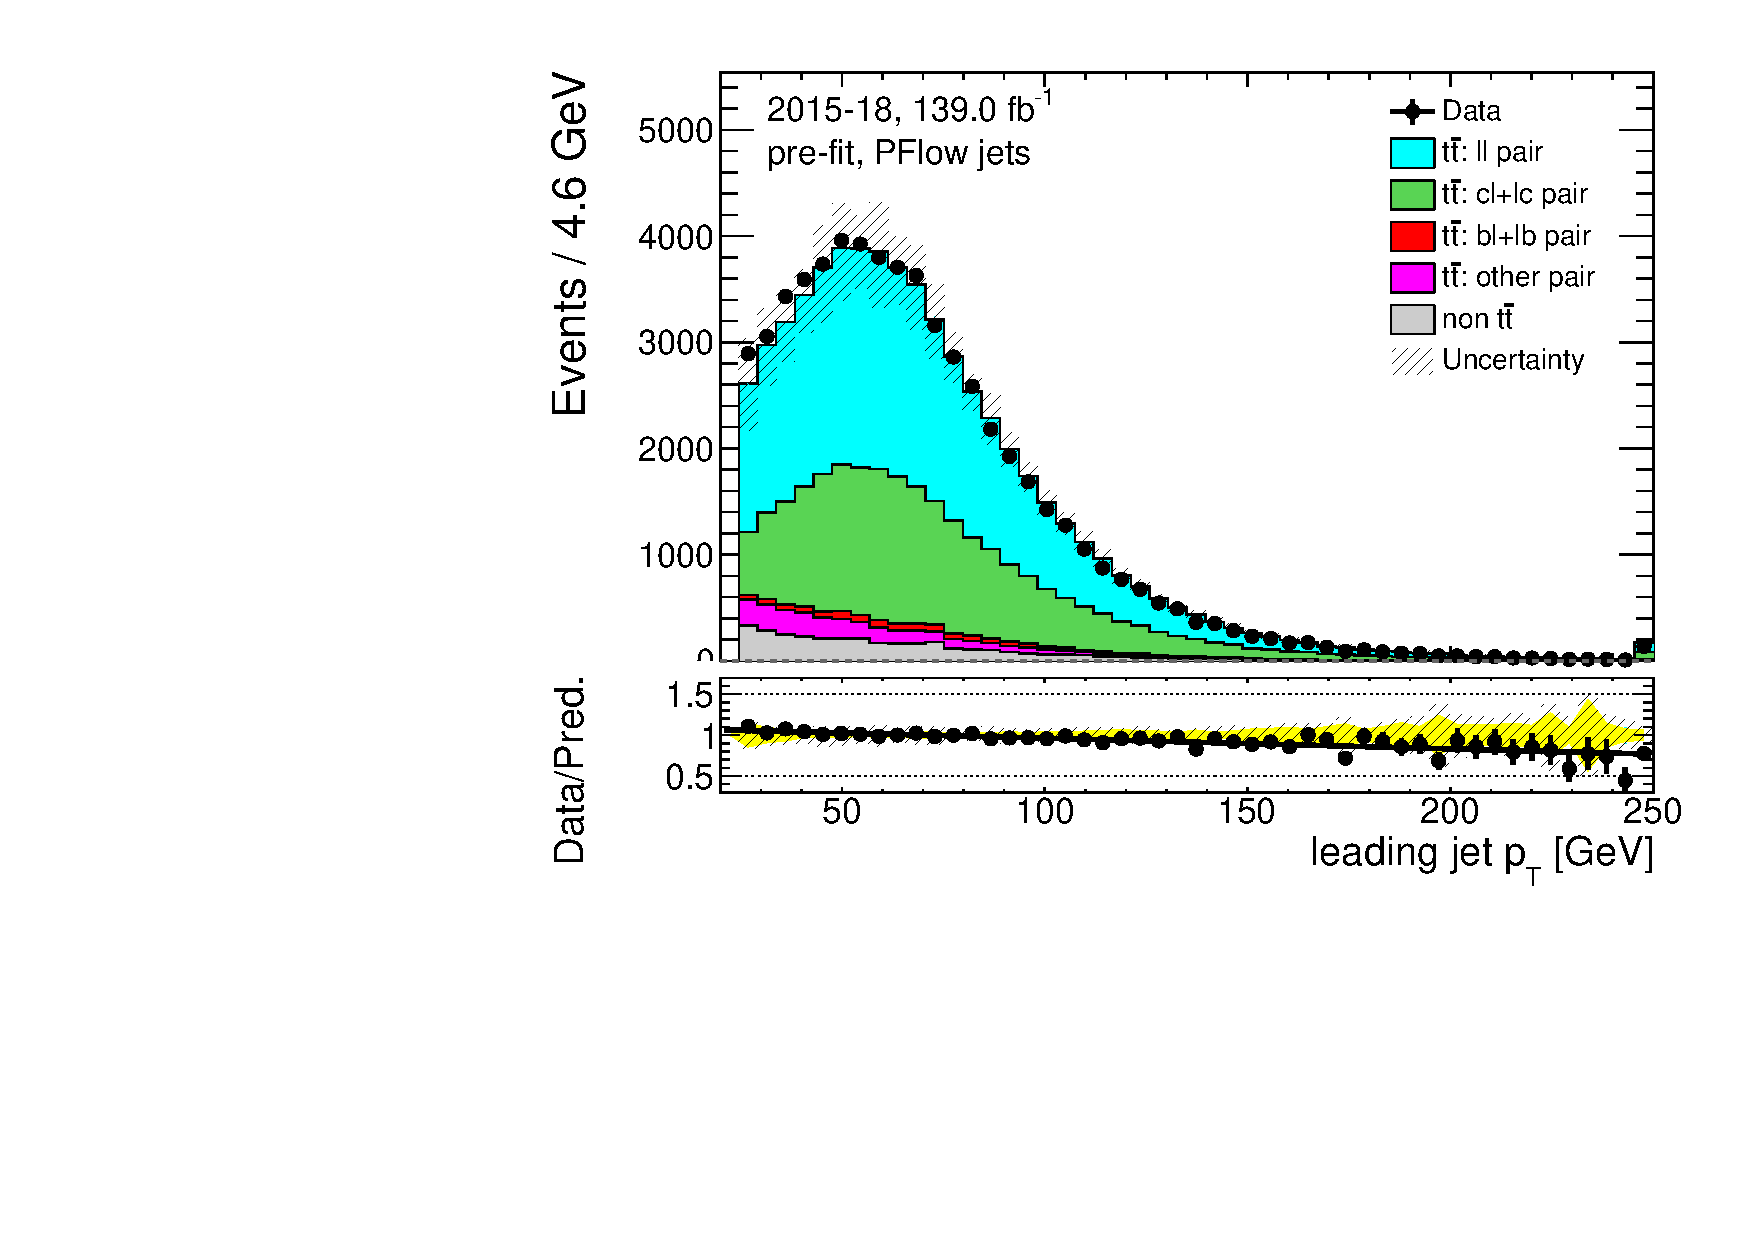
\includegraphics[width=0.45\textwidth]{FTAG_plots/pretagNoRwLowpTPFlowall/DataMC_h_J0_pt.pdf}
	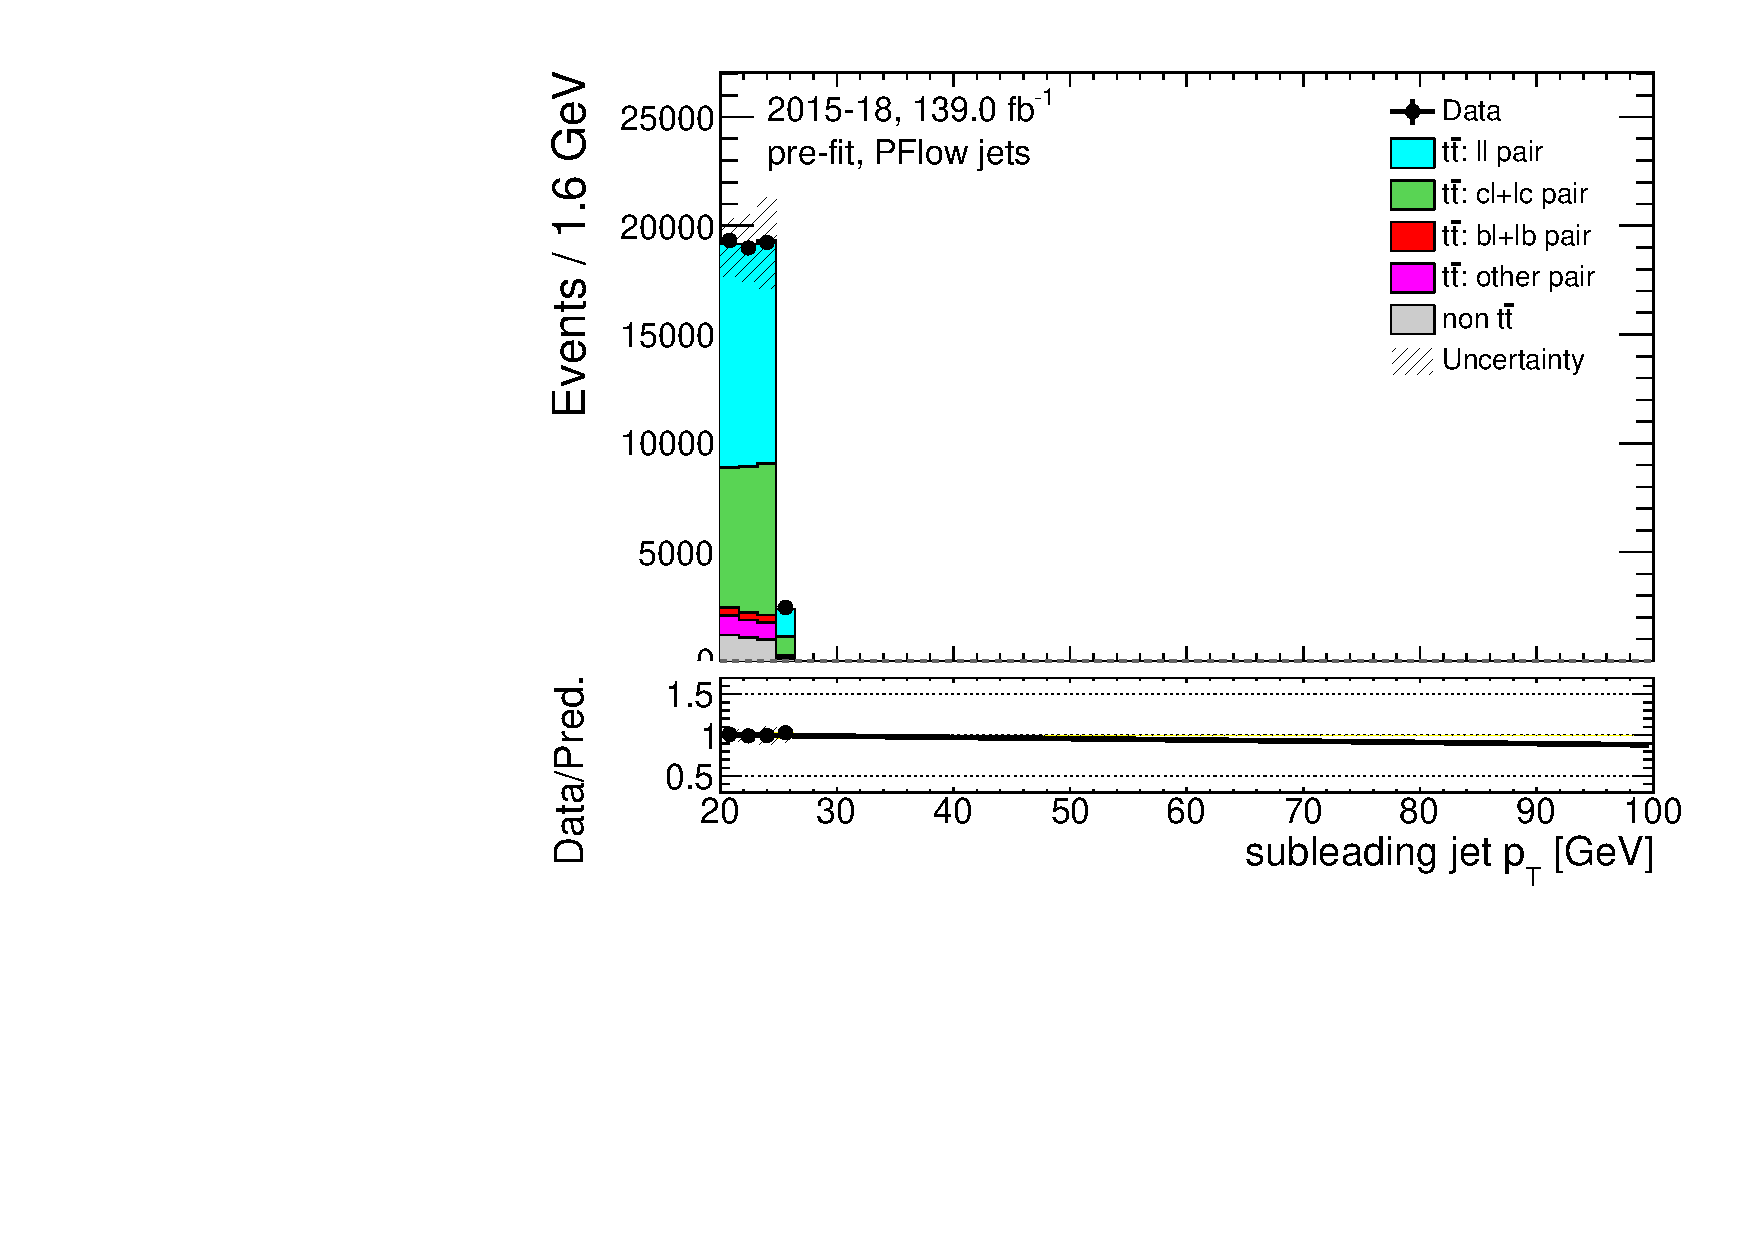
\includegraphics[width=0.45\textwidth]{FTAG_plots/pretagNoRwLowpTPFlowall/DataMC_h_J1_pt.pdf}\\
	\caption{Low-\pt\ selection: data versus simulation of the 
	PFlow $W$ jets \pt. }
	\label{fig:kinematic_distributions_lowpT}
\end{figure}


\subsubsection{High-$p_T$ selection}
\label{high_pt_selection}
It has been observed that in the previous calibrations that the statistics 
are relatively low for the high-\pt\ region (e.g.\ jet $\pt\ > 100$~GeV). 
Therefore, the author has worked on an othorgonal selection to improve this situation.
Instead of requiring events to have exactly 4 jets, events are required to 
have at least 5 jets with $p_{T} > 25$~GeV, in which at least 
1 jet with $\pt\ > 70$~GeV. Other than that, all 
requirements for the selection remain the same. 


The choice of cut value at $70$~GeV is based on the
study shown in the following. 
The effect on the \cjet\ purity and the potential statistical gain is investigated, 
where the \cjet\ purity is defined as:
\begin{equation}
\cjetineq\ \rm{purity} = \frac{N_{\rm{true}\ \cjetunder}}{N_{\rm{all}}},
\end{equation}
where $N_{\rm{true}\ \cjetunder}$ stands for the number of events with a 
true \cjet\ from the $W$ decay, and $N_{\rm{all}}$ stands for the number of all events. 
The ideal situation is the high-\pt\ selection will maximally increase the 
statistics while mininally decreasing the \cjet\ purity, therefore a figure of merit $P^{\rm{Cut}}$
is defined as:
\[P^{\rm{Cut}} = \frac{\sum_i{\rm{Gain\ in\ stats}^2_i}}{\sum_i{\cjetineq \rm{purity}^2_i }}, \]
where i stands for the number of bins. The "Gain in stats" stands for increase in 
statistics and it's summed over all bins in Figure \ref{fig:cutvalue}.
The \cjet\ purity and the statistical gain are calculated for 4 different cut 
values as shown in Figure \ref{fig:cutvalue}, comparing with the cut value of 0. 
The value of $70$~GeV is chosen as it gives the highest value of $P^{\rm{Cut}}$. 


\begin{figure}[!h]
	\centering
	\begin{subfigure}[t]{.38\linewidth}
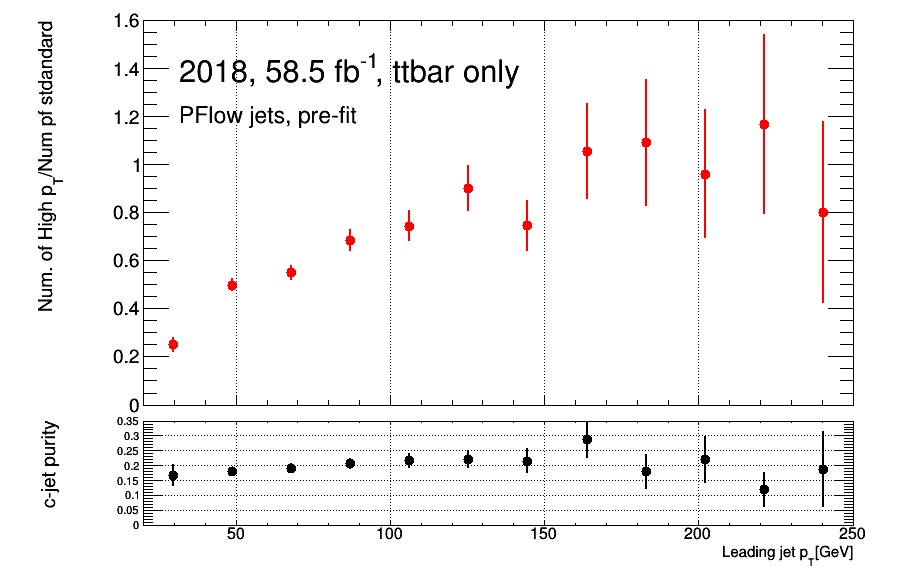
\includegraphics[width=1\textwidth]{FTAG_plots/stat_gains/statsgain_0GeV.png}
\caption{No cut}
\end{subfigure}
\begin{subfigure}[t]{.38\linewidth}
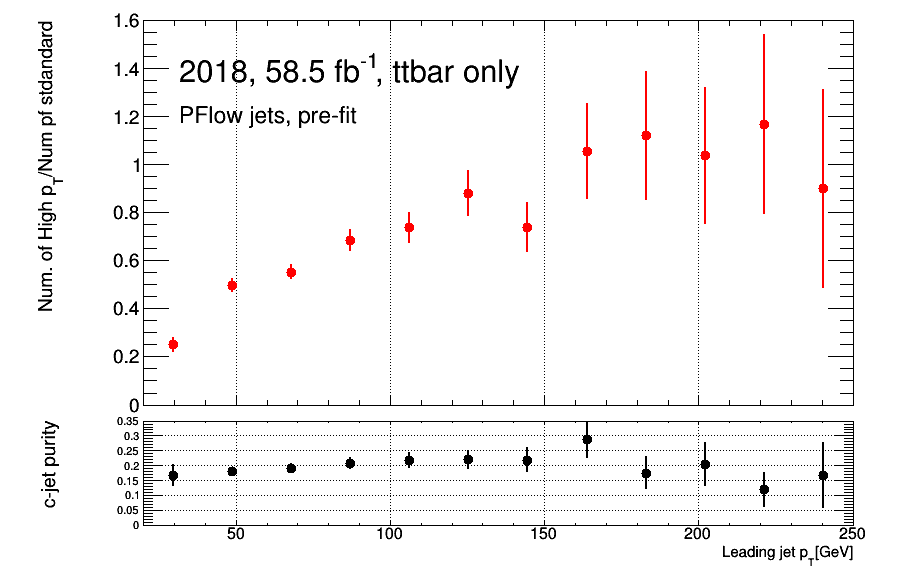
\includegraphics[width=1\textwidth]{FTAG_plots/stat_gains/statsgain_40GeV.png}
\caption{Cut value: 40 GeV}
\end{subfigure}
\begin{subfigure}[t]{.38\linewidth}
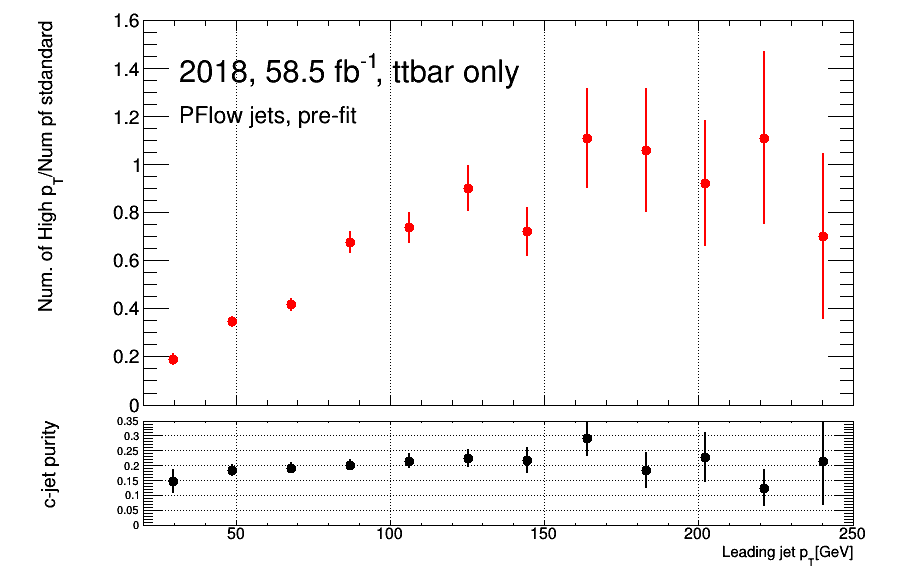
\includegraphics[width=1\textwidth]{FTAG_plots/stat_gains/statsgain_70GeV.png}
\caption{Cut value: 70 GeV}
\end{subfigure}
\begin{subfigure}[t]{.38\linewidth}
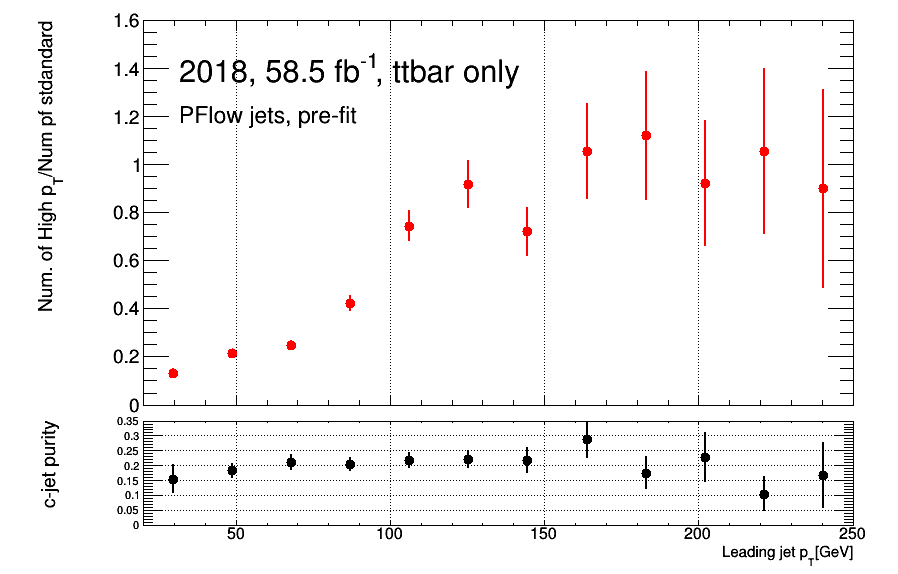
\includegraphics[width=1\textwidth]{FTAG_plots/stat_gains/statsgain_90GeV.png}
\caption{Cut value: 90 GeV}
\end{subfigure}
\begin{subfigure}[t]{.38\linewidth}
\centering
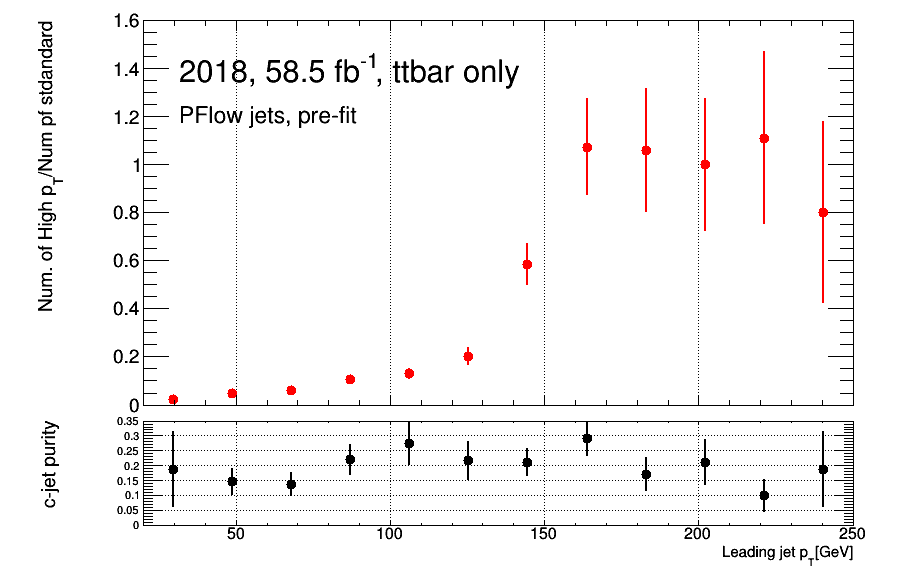
\includegraphics[width=1\textwidth]{FTAG_plots/stat_gains/statsgain_140GeV.png}
\caption{Cut value: 140 GeV}
\end{subfigure}

\caption{Comparison of different cut values in terms of gain in stats and \cjet\ purity.}
\label{fig:cutvalue}
\end{figure}

\begin{table}[ht]
	\centering
	\small
	\setlength\tabcolsep{5pt} 
	\newcolumntype{C}{ @{}>{${}}c<{{}$}@{} }
	\begin{tabular}{|r *2{|rCr}| }
	\hline
	& \multicolumn{3}{|c|}{PFlow jets} & \multicolumn{3}{c|}{Track jets} \\
	\hline
	
	Data    &     98273  &           &   &        83957   &              &   \\ 
	\ttbar\ &    99430 &\pm&  120 &        87476 &\pm&  110     \\
	Non \ttbar\   &      1842  &\pm&  21 &          1570  &\pm&  20     \\
	\hline
	Data/MC &      0.97  &\pm&  0.003   &     0.94  &\pm&  0.003       \\
	\hline

	\end{tabular}
	\vspace{0.2cm}
	\caption{High-\pt\ selection: prefit comparison of the number of events in data and in 
	simulation considering the PFlow $W$ jets and the VR-Track jets.}
	\label{tab:yields_highpT}
	\end{table}

\begin{figure}[!h]
	\centering
	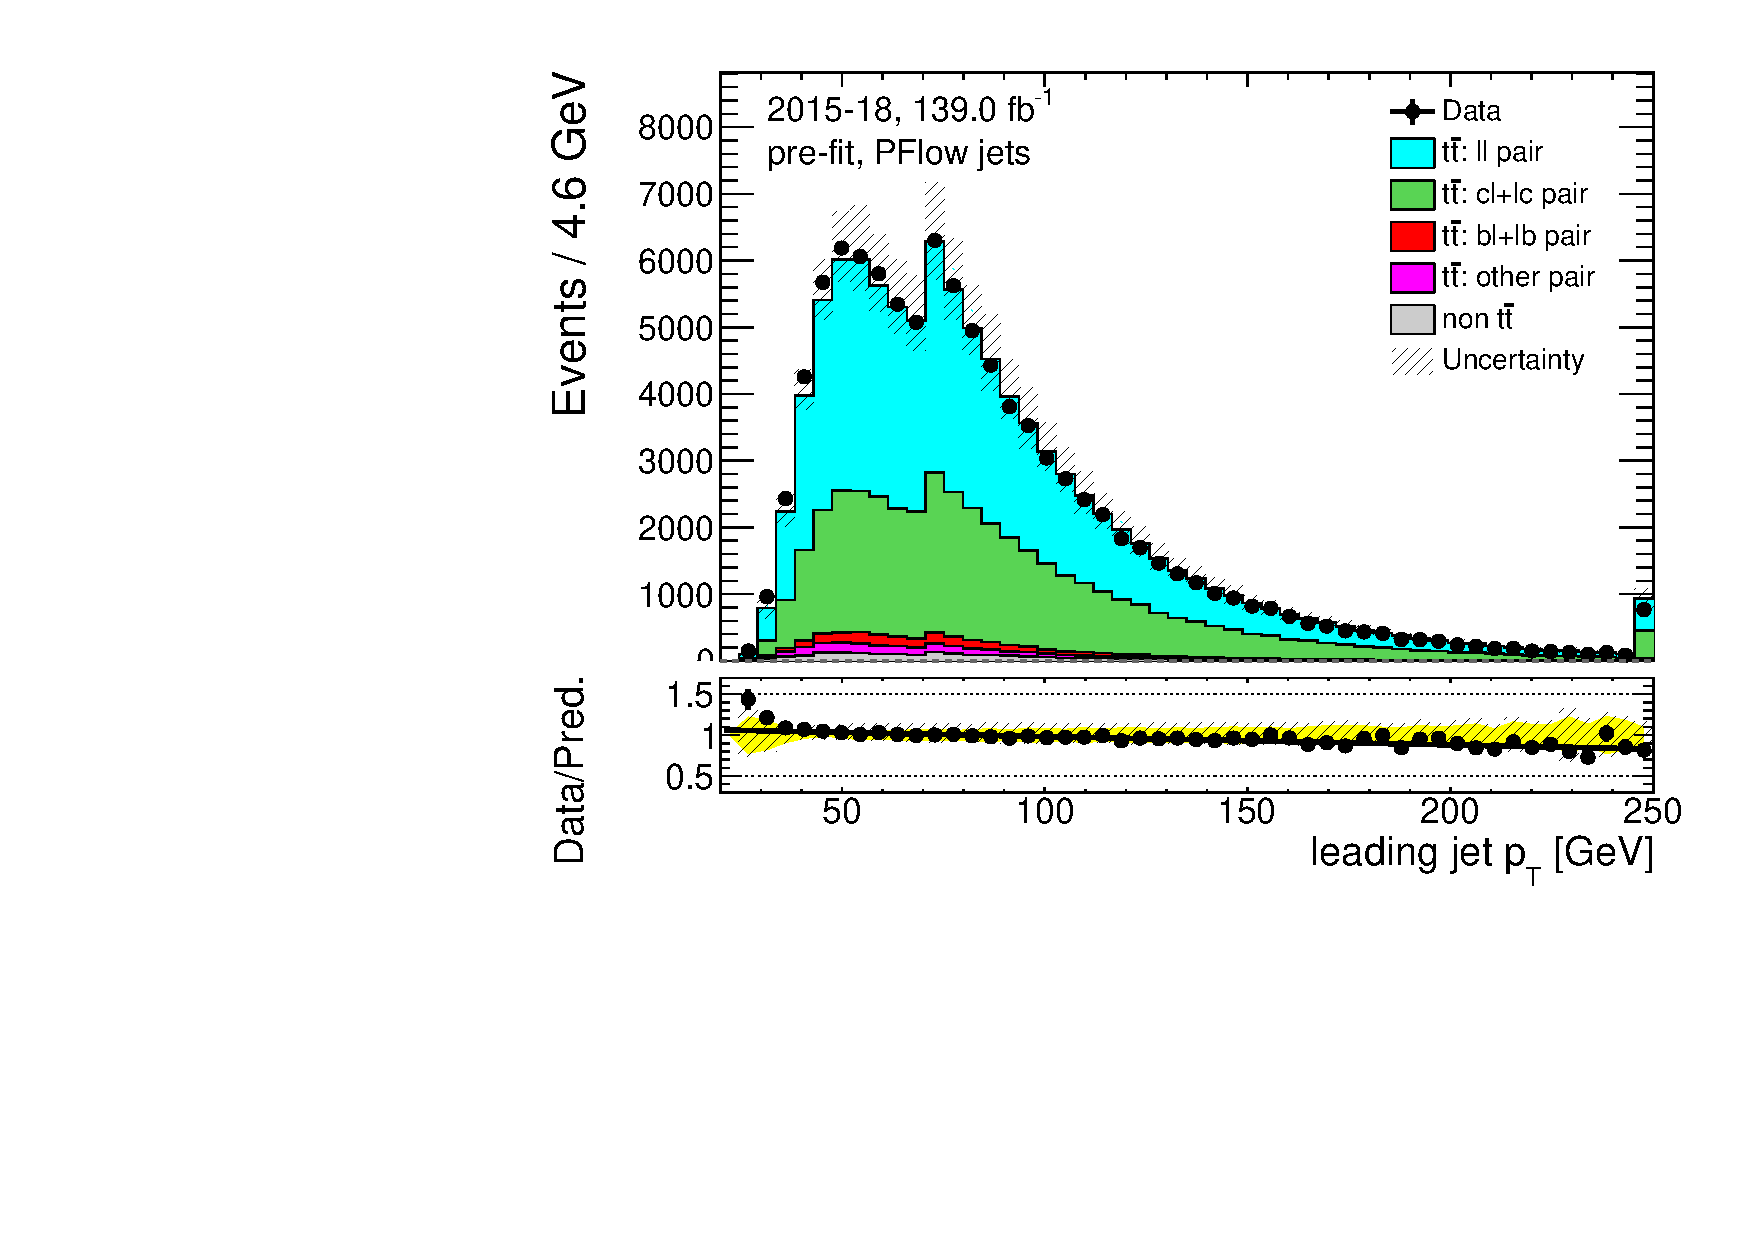
\includegraphics[width=0.45\textwidth]{FTAG_plots/pretagNoRwnewonlyPFlowall/DataMC_h_J0_pt.pdf}
	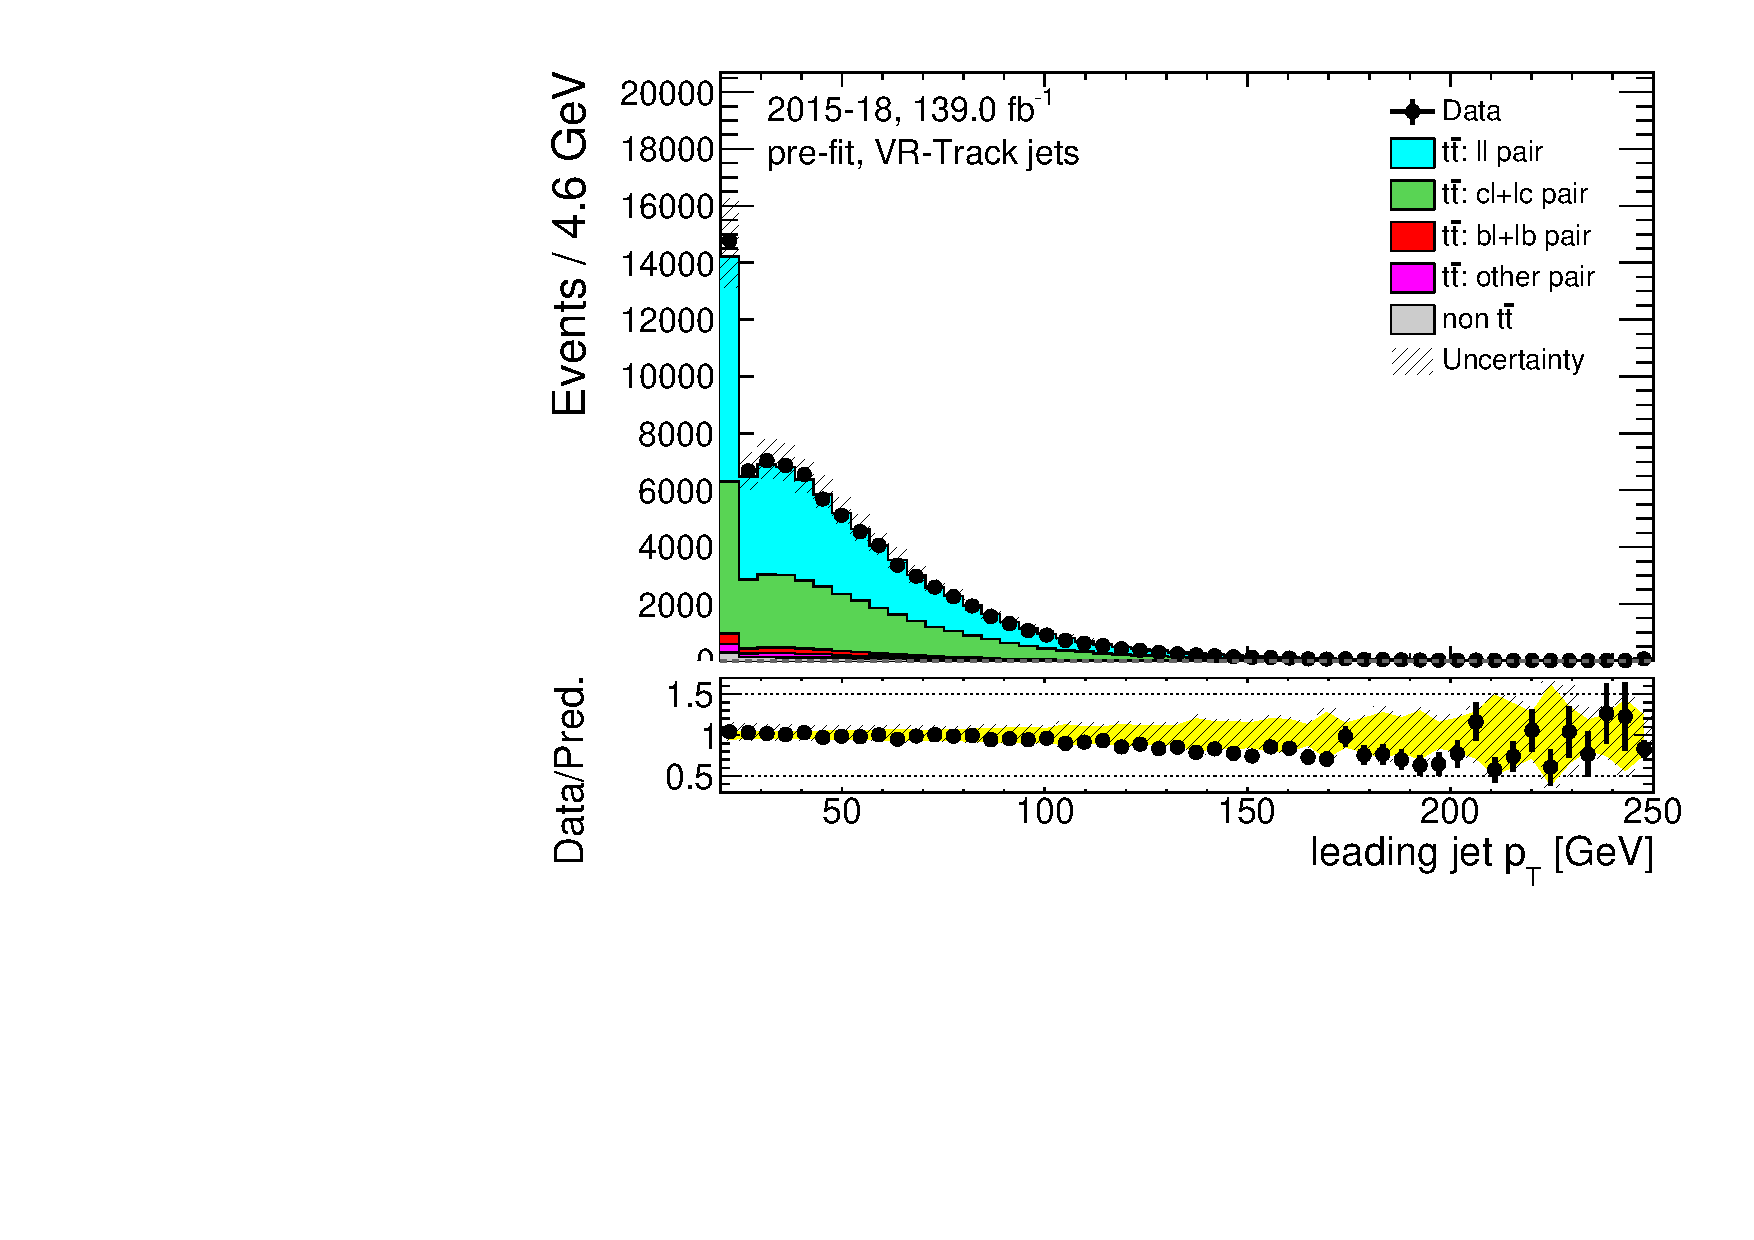
\includegraphics[width=0.45\textwidth]{FTAG_plots/pretagNoRwnewonlyVRJetsall/DataMC_h_J0_pttrackjet.pdf}\\
	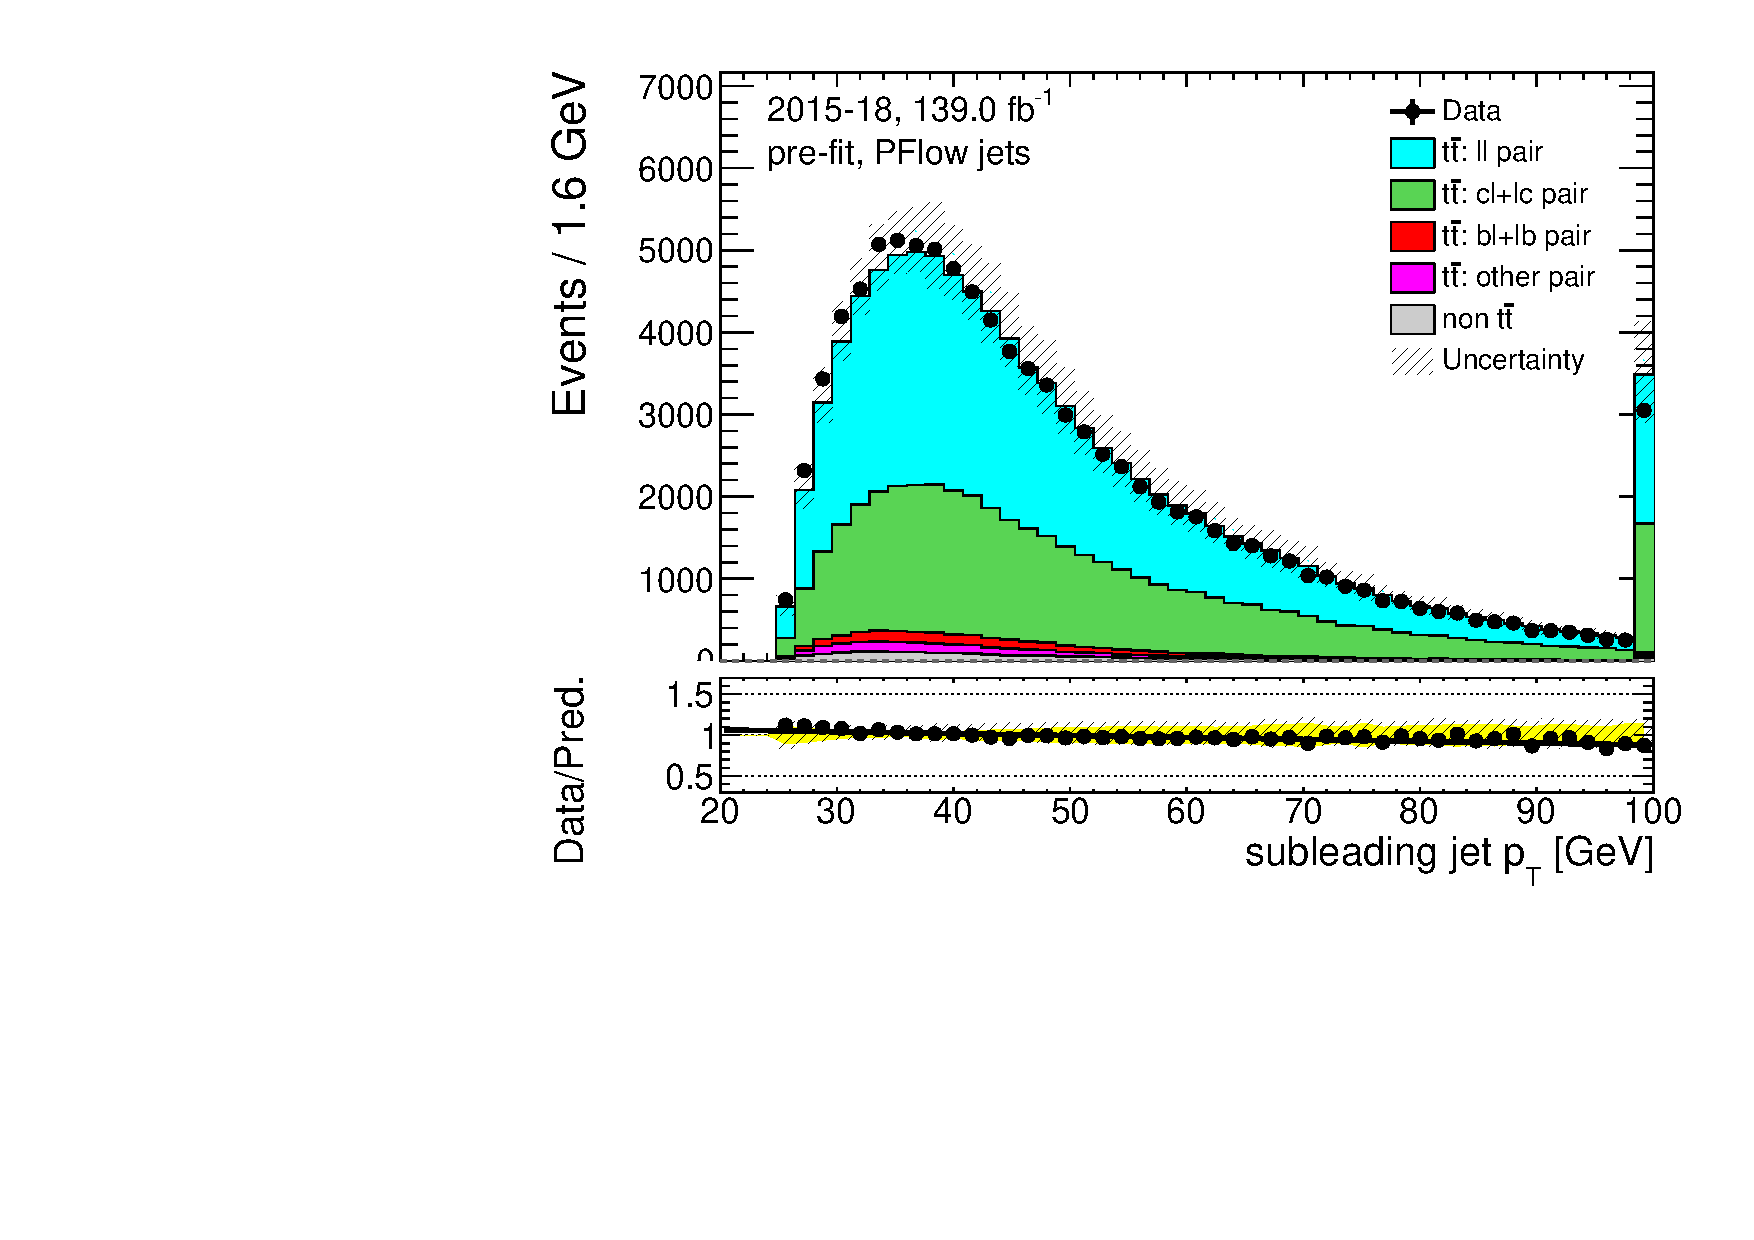
\includegraphics[width=0.45\textwidth]{FTAG_plots/pretagNoRwnewonlyPFlowall/DataMC_h_J1_pt.pdf}
	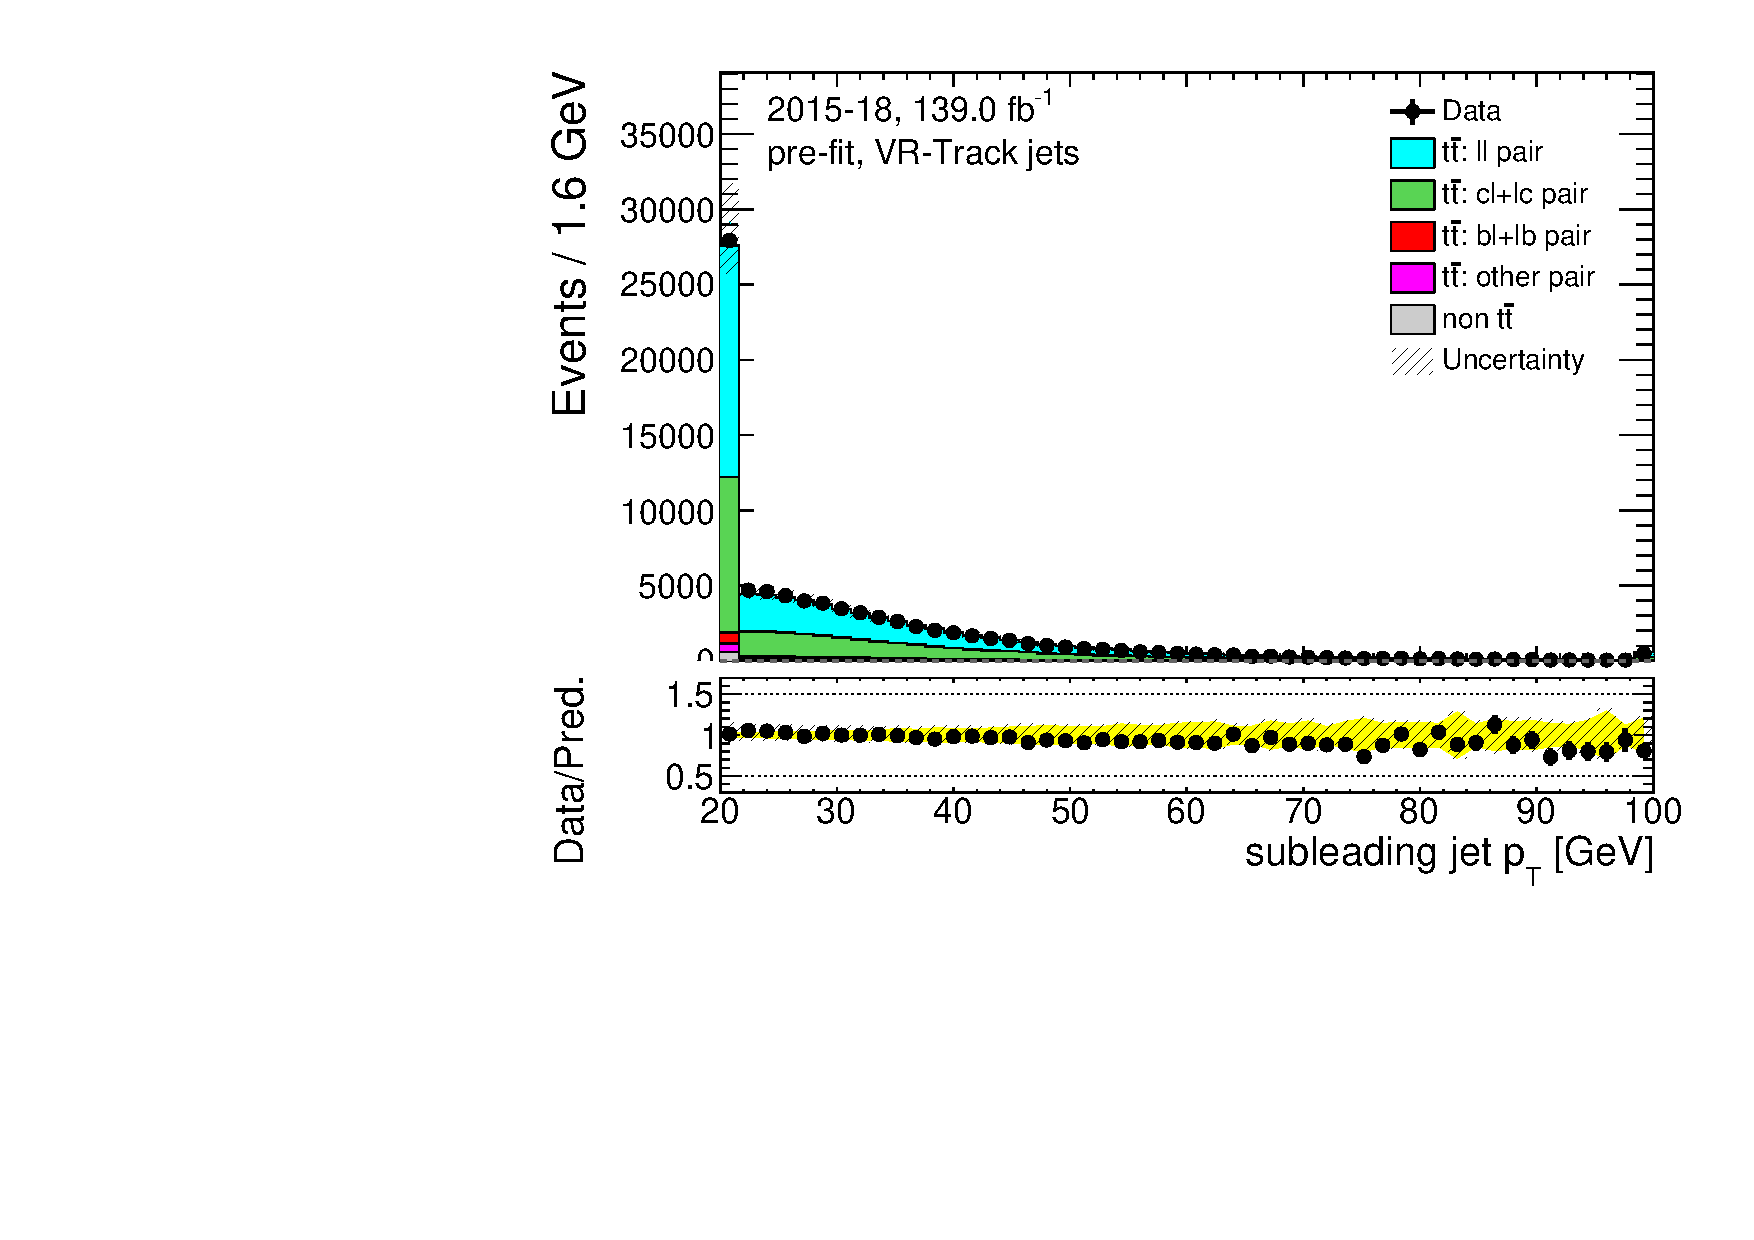
\includegraphics[width=0.45\textwidth]{FTAG_plots/pretagNoRwnewonlyVRJetsall/DataMC_h_J1_pttrackjet.pdf}\\
	\caption{High-\pt\ selection: data versus simulation of $W$ jets \pt\ for 
	PFlow jets in the left column and for VR-Track jets in the right column.}
	\label{fig:kinematic_distributions_highpT}
\end{figure}
	

The yields of the data and the MC are given in Table \ref{tab:yields_highpT}. 
An example of the \pt\ distributions before any tagging or fitting, applying 
the high-\pt\ selection is shown in Figure \ref{fig:kinematic_distributions_highpT}. 
In general the event statistics improve about 80\% in region with \pt\ > 70 GeV as desired.
More plots can be found in Appendix \ref{sec:appendix_highpT_selection}.




\subsubsection{Combined selection}
\label{combined_selection}
As the standard selections, low-\pt\ selection and high-\pt\ selection are othorgonal 
to each other, all the selections are combined to provide the maximum range 
and statistics for the calibration. 
The yields of the data and the MC are given in Table \ref{tab:yields_combined}, 
an example of the \pt\ distributions before any tagging or fitting and 
after the combined selection is shown in Figure \ref{fig:kinematic_distributions_combined}. More plots 
can be found in Appendix \ref{sec:appendix_combined_selection}.

\begin{table}[ht]
	\centering
	\small
	\setlength\tabcolsep{5pt} 
	\newcolumntype{C}{ @{}>{${}}c<{{}$}@{} }
	\begin{tabular}{|r *2{|rCr}| }
	\hline
	& \multicolumn{3}{|c|}{PFlow jets} & \multicolumn{3}{c|}{Track jets} \\
	\hline
	Data          &    385378           &      &        &   302308         &  &     \\  
	\ttbar\       &      383520   &\pm&  230 &            302690 &\pm&  200   \\
	Non \ttbar\         &        12420  &\pm&  120 &             8570  &\pm&  100     \\
	Data/MC       &        0.973  &\pm&  0.002 &           0.971 &\pm&  0.002          \\
	\hline

	\end{tabular}
	\vspace{0.2cm}
	\caption{Combined selection: prefit comparison of the number of events in data and in 
	simulation considering the PFlow jets and the VR-Track jets for an inclusive
	selection.}
	\label{tab:yields_combined}
	\end{table}

\begin{figure}[!h]
		\centering
		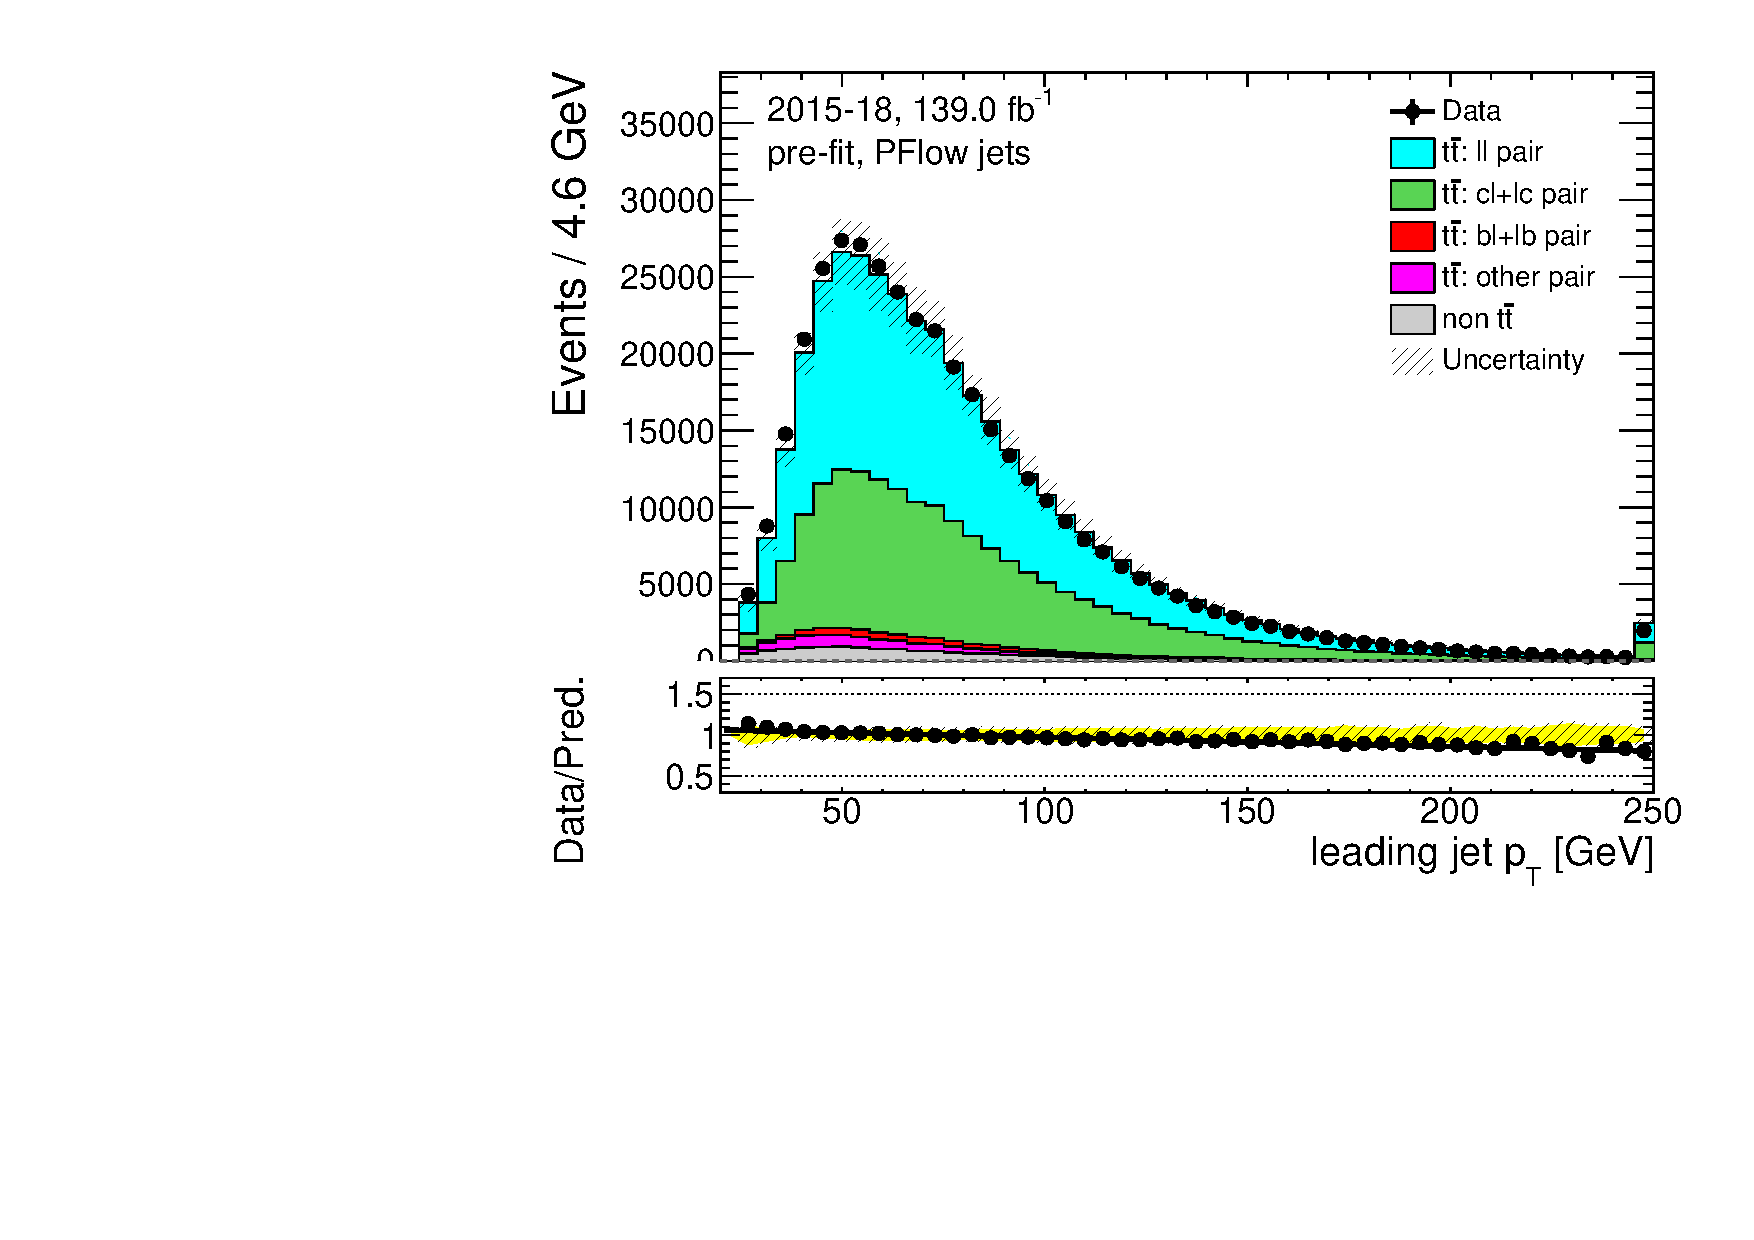
\includegraphics[width=0.45\textwidth]{FTAG_plots/pretagNoRwwithhighpTPFlowall/DataMC_h_J0_pt.pdf}
		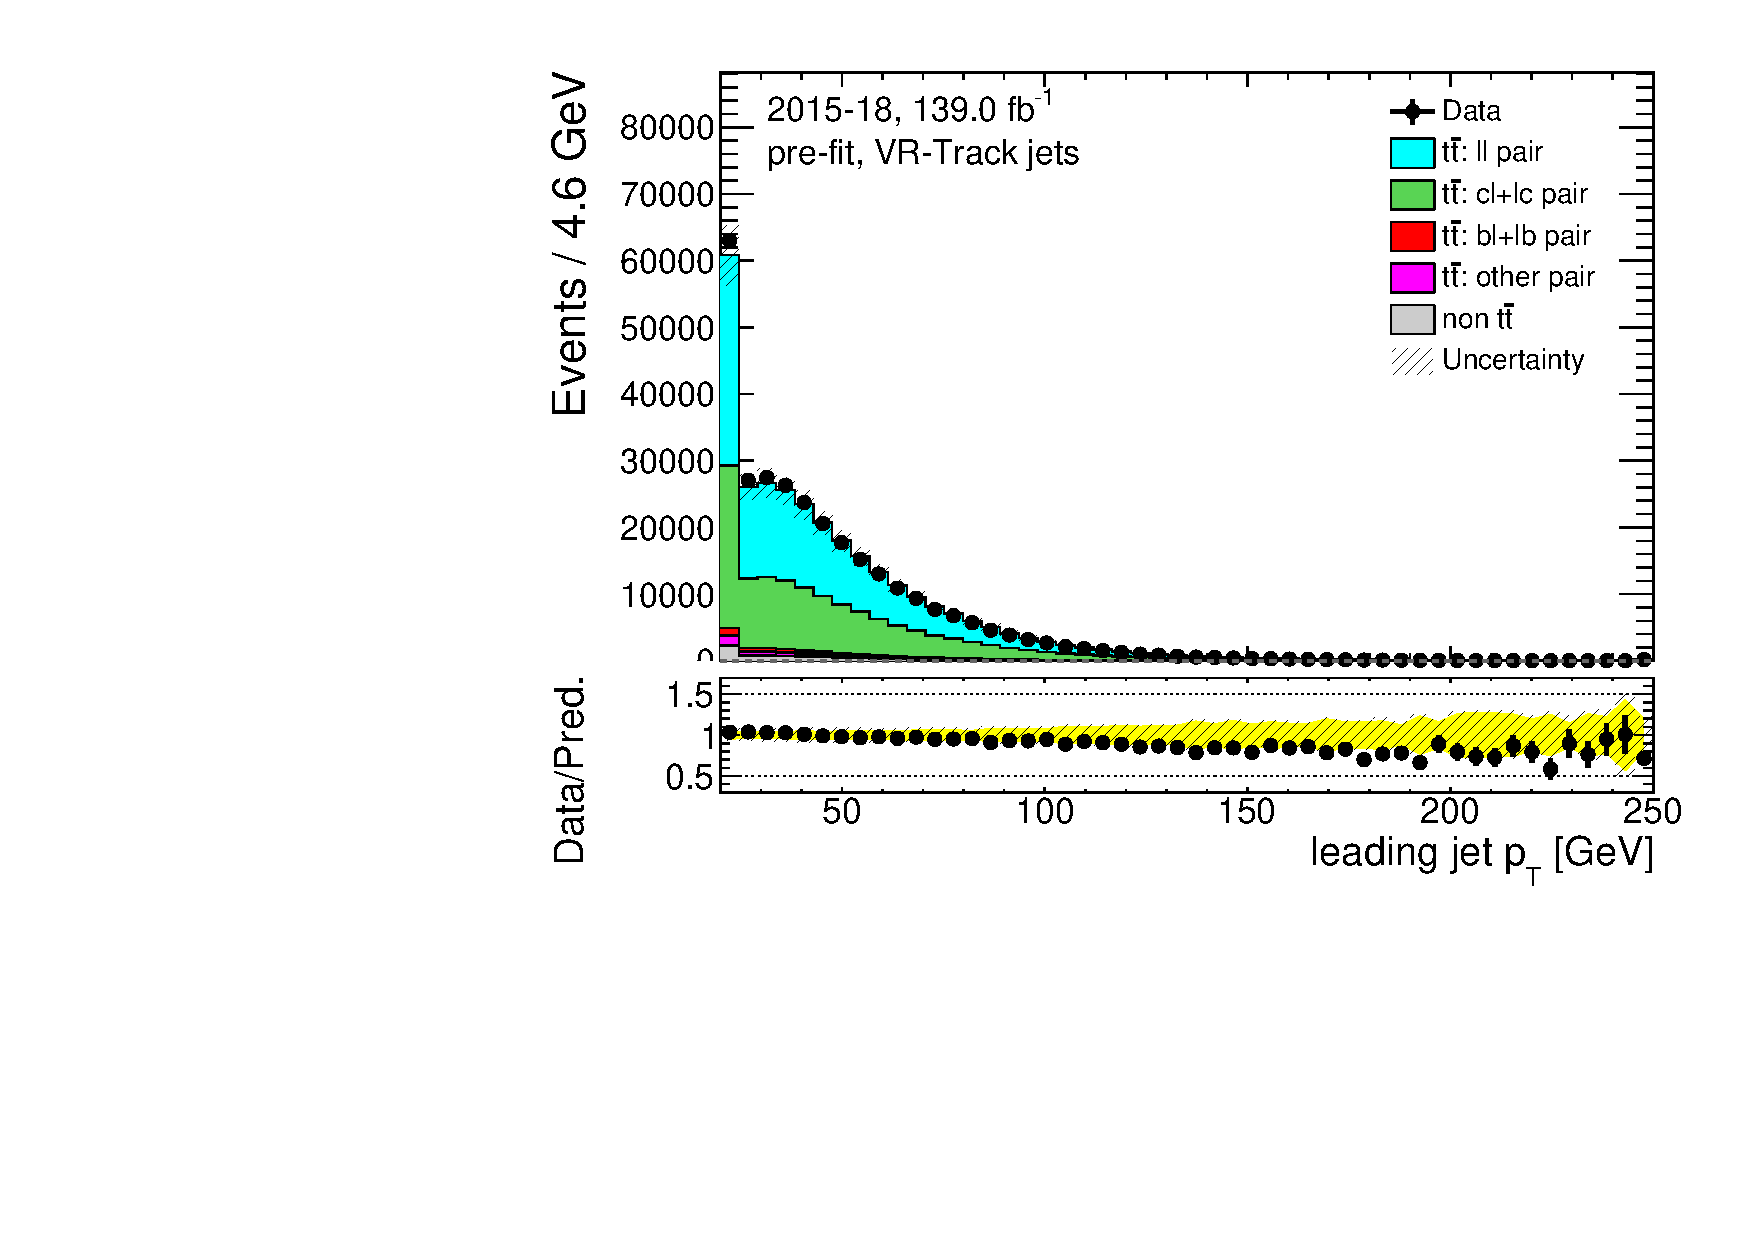
\includegraphics[width=0.45\textwidth]{FTAG_plots/pretagNoRwwithhighpTVRJetsall/DataMC_h_J0_pttrackjet.pdf}\\
		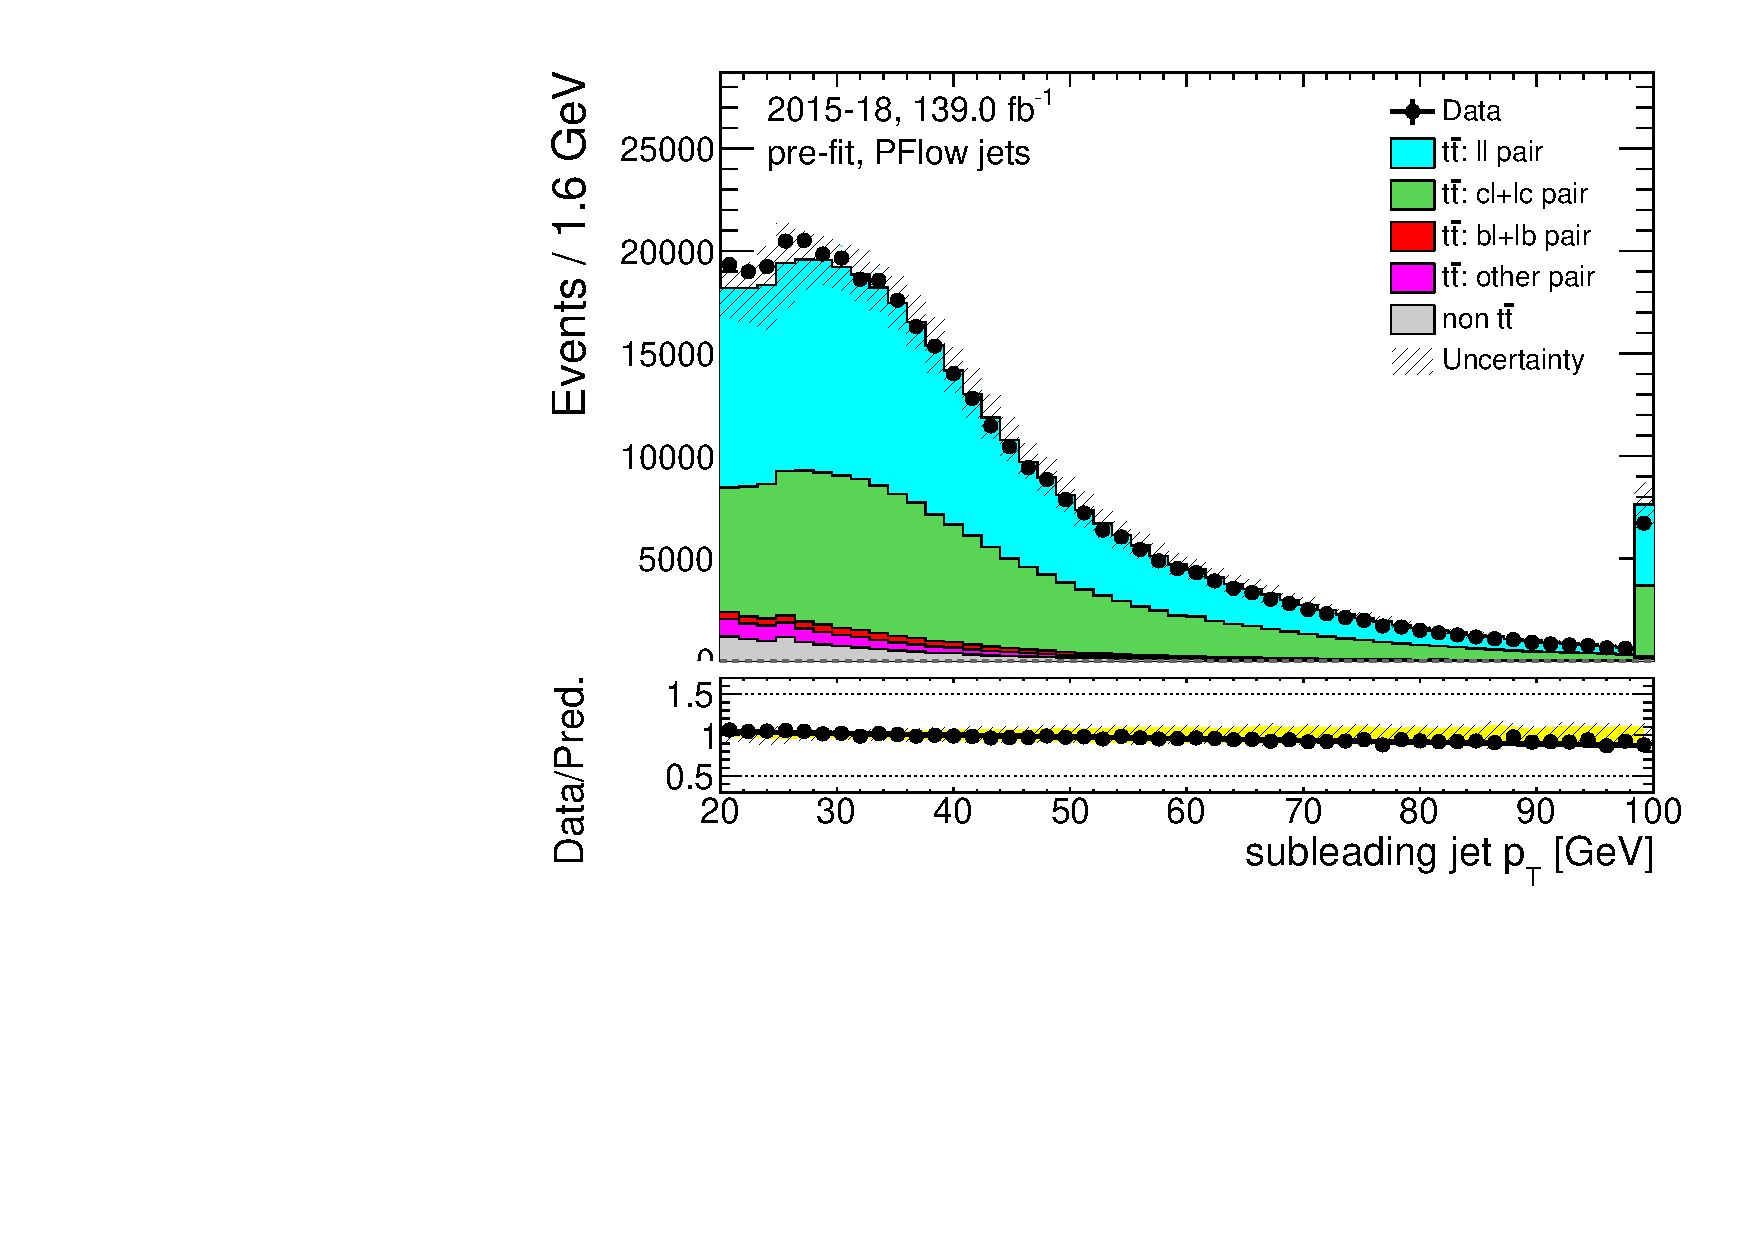
\includegraphics[width=0.45\textwidth]{FTAG_plots/pretagNoRwwithhighpTPFlowall/DataMC_h_J1_pt.pdf}
		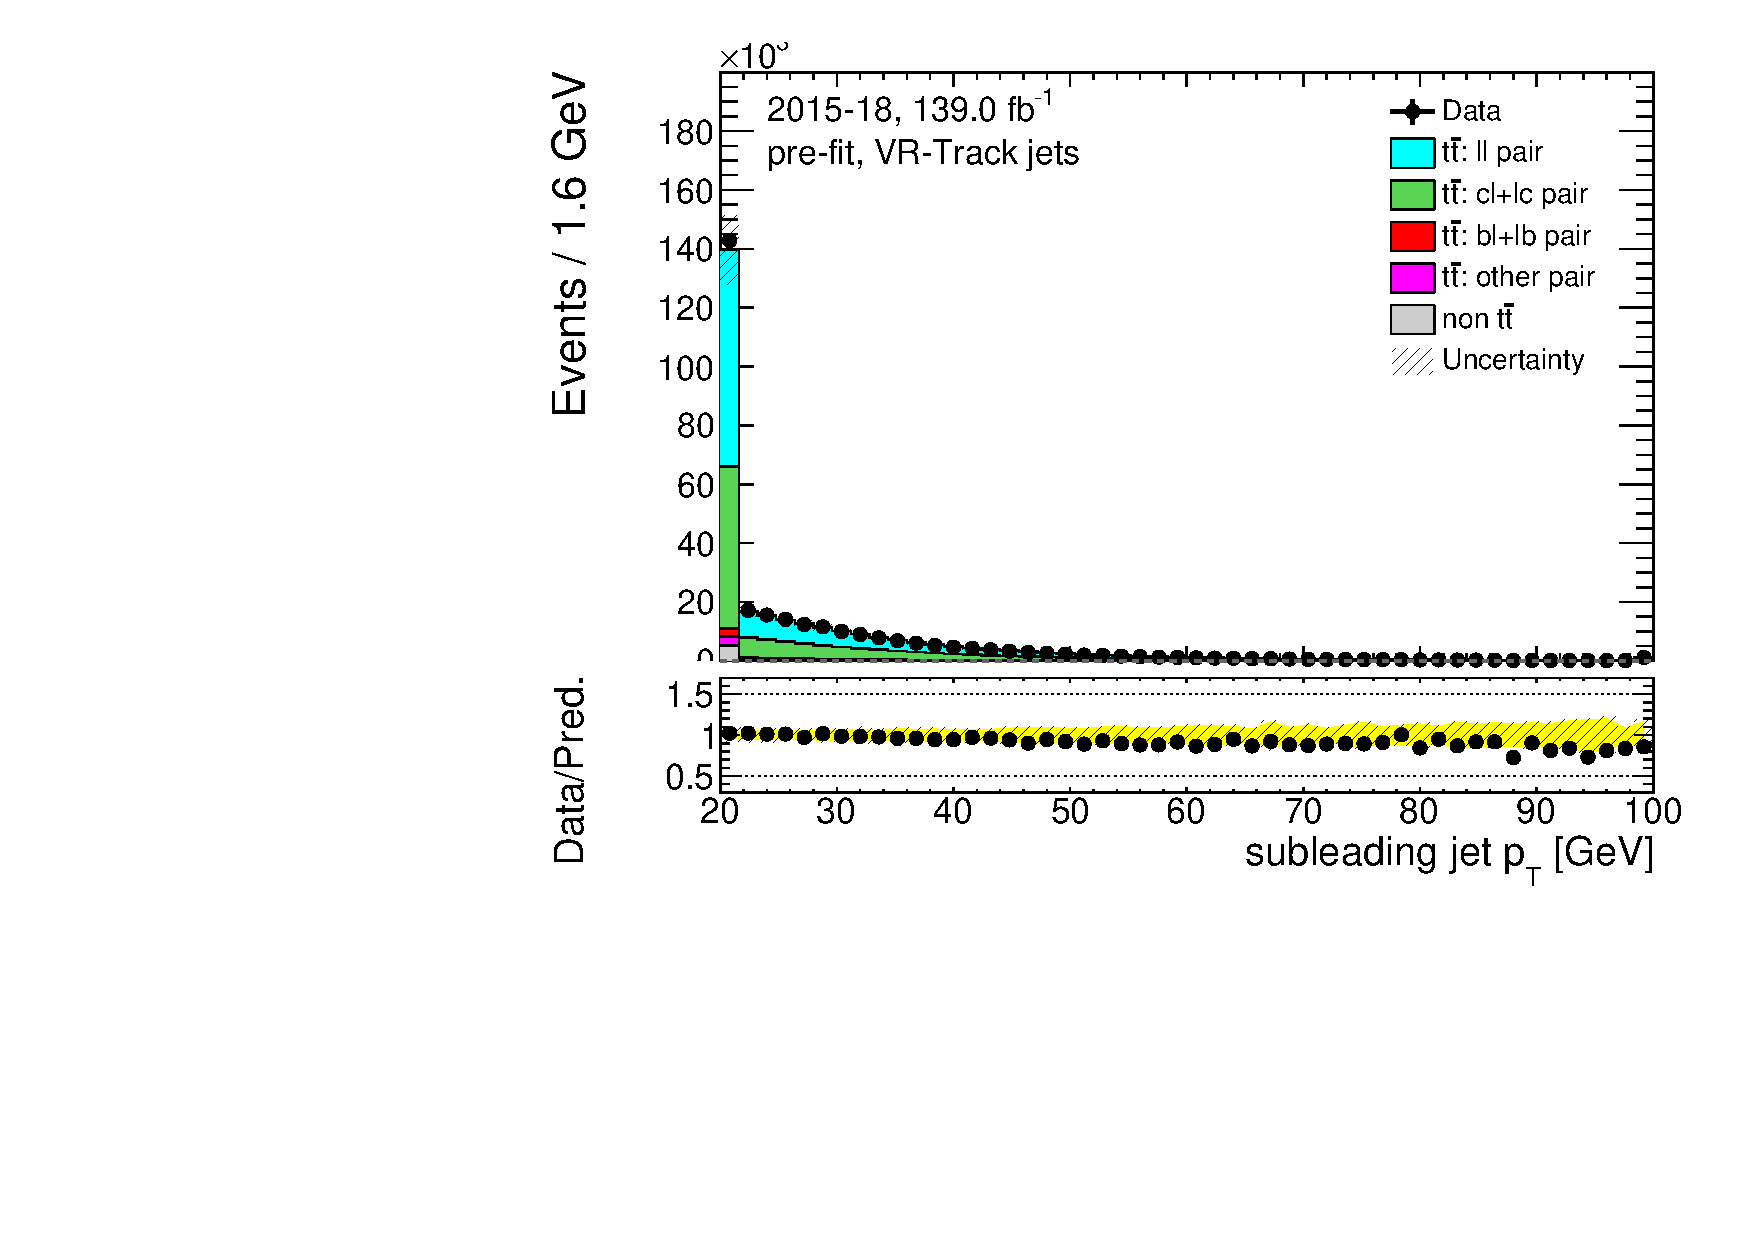
\includegraphics[width=0.45\textwidth]{FTAG_plots/pretagNoRwwithhighpTVRJetsall/DataMC_h_J1_pttrackjet.pdf}\\
		\caption{Combined selection: data versus simulation of $W$ jets\pt\ for 
		PFlow jets in the left column and for VR-Track jets in the right column.}
		\label{fig:kinematic_distributions_combined}
\end{figure}
		

\subsection{Systematic uncertainties}
\label{sec:FTAG_systematics}
The systematic uncertainties considered and propagated in this calibration 
can be broadly categorised into experimental and modelling systematic uncertainties. 
\subsubsection{Experimental uncertainties}
TODO: refer to the analysis Part
Experimental uncertainties are related to the detector and estimated using 
data-driven methods or MC simulations. 
The lepton energy scale and resolution are corrected to 
provide better agreement between MC predictions and data, uncertainties 
due the corrections are considered. Uncertainties are taken into account on the 
electron and muon trigger, identification and reconstruction efficiencies, and for 
uncertainties associated with the isolation requirements. 

The jet energy scale (JES) uncertainty depends on $p_T$ and $\eta$ and 
takes into account uncertainties due to pile-up effects. Uncertainties on the jet energy resolution (JER) 
are taken into account. Uncertainties on the energy scale and resolution of 
the electrons, muons, jets and taus are propagated to the calculation of the \MET, 
which also has additional dedicated uncertainties on the scale, resolution, and 
reconstruction efficiency of tracks not associated to any of the reconstructed objects,
 along with the modelling of the underlying event. Uncertainties on the $b$-tagging (mis-tagging) 
 probabilities for $b$ (light) jets are considered both for the tagging jets assigned to the $b$ quark 
 from the top decay and for the jets associated to the hadronically decaying $W$ boson.
Supporting material for this section can be found in the appendix, Tab.\ref{tab:systematics}.
%The uncertainty on these corrections is taken into account as a shape-dependent systematic uncertainty in the final fit of the backgrounds and signal models.

\subsubsection{Modelling uncertainties} 
The uncertaity due to different choices of the parton shower models is estimated by comparing
the MC samples generated with nominal parton shower model and with the 
alternative parton shower model.
More specifically, it is derived 
by comparing the prediction from \powheg interfaced either to \pythia or \Herwigpp. 
The uncertainty due to additional radiation in 
the initial state and the final state is estimated by comparing the nominal MC samples with the MC samples 
with alternative scale of renormalisation and factorisation.
The uncertainty on modelling of initial state radiation (ISR) is assessed with two alternative \powhegpythia 
samples. The samples include one with an increase in radiation which has the renormalisation and 
factorisation scales decreased by a factor of two and the \textit{hdamp} parameter doubled 
(which controls the \pt\ of the first additional emission), while 
the sample with a decrease in radiation has the scales increased by a factor of two. 
In all cases, MC-to-MC SFs are taken into account.
In addition, the uncertainty due to the
variations samples being produced by fast simulation while the nominal samples being 
produced full simulation is also considered.
The comparisons of 
the nominal \ttbar\ sample and the samples with each systematic uncertainty 
are shown in Table \ref{tab:modelling_syst}. 



\begin{table}[ht]
	\centering
	\small
	\setlength\tabcolsep{5pt} 
	\newcolumntype{C}{ @{}>{${}}c<{{}$}@{} }
	\begin{tabular}{|r *2{|rCr|r}| }
	\hline
	& \multicolumn{4}{|c|}{PFlow jets} & \multicolumn{4}{c|}{Track jets} \\
	\hline
	& \multicolumn{3}{c|}{Yields} & \specialcell{Ratio of \\difference to \\nominal sample} & \multicolumn{3}{c|}{Yields} & \specialcell{Ratio of \\difference to\\ nominal sample} \\
	\hline
	\ttbar\ Nominal &	 385378  &\pm&  230 &         &   	  302690 &\pm&  200   &  \\
	Data/MC         &        0.973  &\pm&  0.002 &      &     0.971 &\pm&  0.002 &         \\
	\hline
	\ttbar\ AF2     &    386260  &\pm&  250  &  0.716\% &     304860  &\pm&  230  &  0.716\%\\
	DATA/MC(AF2)    &    0.967  &\pm&  0.002  &          &    0.965  &\pm&  0.002   &      \\              
	\hline
	\ttbar\ ISR     &    377130  &\pm&  220  & -1.665\% &     297960  &\pm&  200  & -1.562\%\\     
	DATA/MC(ISR)    &    0.989  &\pm&  0.002  &          &    0.986  &\pm&  0.002   &  \\       
	\hline
	\ttbar\ \Herwig &    331960  &\pm&  220  & -13.443\%&     259940  &\pm&  190  & -14.123\%\\ 
	DATA/MC(\Herwig)&    1.119  &\pm&  0.002  &          &    1.126  &\pm&  0.002   &\\                
	\hline
	\end{tabular}
	\vspace{0.2cm}
	\caption{Comparison of the number of events in data and in 
	simulation considering the PFlow jets and the VR-Track jets for an inclusive
	selection. The uncertainty due to the variations samples being produced 
	by fast simulation is included in the table as \ttbar\ AF2. }
	\label{tab:modelling_syst}
	\end{table}


\subsection{Under-estimation of $t\bar{t}$ + Heavy flavour background }
Depsite the fact that the true nature of most of the reconstructed $W$ jets are either 
\cjets\ or light jets, there is still a very small amount of them are true \bjets. 

There are two main sources of these true \bjets. The first is a $W$ boson 
decays to a $b$ and a $c$ quark. The second is 
when the $t\bar{t}$ plus a gluon process (referred to as \ttbar\ + heavy flavour process)
is selected, and the gluon splits
into a pair a $b$ quarks and one of them is assigned as a $W$ jet. 
The first source can be excluded by requiring no \cjets in the $W$ jets,
meaning the true \bjet\ in the $W$ jets 
can only come from the $t\bar{t}$ + heavy flavour 
process. This process is underestimated by the MC by about 30\% 
for both the PFlow and VR-Track jets collections, as shown in Table \ref{tab:3byields1} 
and Figure \ref{fig:3bplots}, where an extra cut requiring at least one $W$ jet with DL1r $> 8$ 
is added to the combined selection to reject most of the true \cjets and true light jet. 
A more thorough study is done in Ref. \cite{TOPQ-2017-12}, where the mis-modelling 
factor is measured to be $1.25 \pm 0.25$, which is also consistent with the $30\%$ 
mismodelling observed in the previous study. 
Therefore, events in the simulation
in which the top jets and at least one of the $W$ jets are \bjets (referred to as 3 true \bjets\ events), 
are scaled by $1.25 \pm 0.25$.
All results shown in this chapter have this scale factor implemented, 
and the full difference between the simulation before applying this scale factor and 
after is taken as a systematic uncertainty. This uncertainty has been added in quadrature 
to the systematic uncertainties described in Section \ref{sec:FTAG_systematics} 
in all the plots in this chapter.



\begin{table}[ht]
    \centering
	\newcolumntype{C}{ @{}>{${}}c<{{}$}@{} }
	\begin{tabular}{|r *2{|rCr}| }
		\hline
		& \multicolumn{3}{|c|}{PFlow jets} & \multicolumn{3}{c|}{VR-Track jets} \\
		\hline
        Data & 1589& & & 1336  & & \\
         $t\bar{t}$ & 1100  &\pm&  13	& 940  &\pm&  12\\
         Non \ttbar\ 		& 83  &\pm&  6		& 69  &\pm&  5  \\
		 Data/MC 	& 1.34  &\pm&  0.04 & 1.32  &\pm&  0.04 \\
		 \hline
    \end{tabular}
	\caption{Yields of the 2018 data and MC of the combined selection, 
	requiring at least 1 PFlow or track $W$ jet with DL1r > 8 to 
	reject most of the light- and \cjets.}
    \label{tab:3byields1}
\end{table}


\begin{figure}[!h]
    \centering
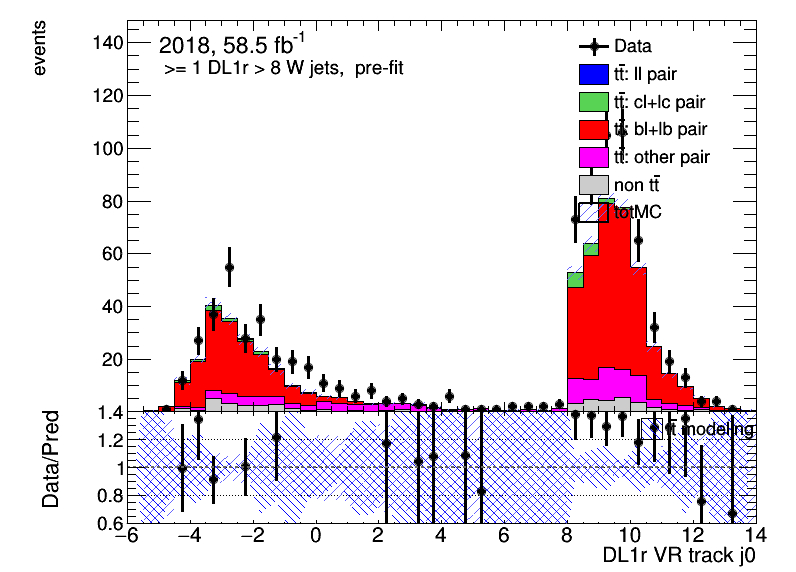
\includegraphics[width=.45\textwidth]{FTAG_plots/3bplots/3bplots.png}
	\caption{The DL1r score distribution of the leading VR-Track jet, 
	requiring at least 1 VR-Track jets have DL1r > 8 to reject most of 
	the light and the $c$ jets, with $t\bar{t}$ modelling and statistical uncertainties. }
    \label{fig:3bplots}
\end{figure}


\subsection{Results}
\label{result}


\subsubsection{Overview}
Four rounds of calibrations have been carried out, containing different 
jet collections, Monte Carlo samples, analysis framework 
and \bjet\ identification algorithm. 
In the latest round, 
the calibration includes the PFlow jet and the VR-Track jet collection, 
and MV2c10, DL1 and DL1r taggers. The low-$p_T$ 
selection and the standard selection are carried out for all four 
calibrations, while the high-$p_T$ selection is only implemented 
in the latest calibration. 

\subsubsection{\btagging\ algorithms output distribution}
The distributions of the \btagging\ algorithm' output of 
the MC and the data of the latest calibration 
(December 2020) are shown in Figure \ref{fig:taggers_PFlow} for the PFlow jets and 
Figure \ref{fig:taggers_VRJets} for the VR-Track jets, 
combining the standard selection, low \pt\ and the high-$p_T$ selection. 
In these figure, the data events are compared against the simulation.
The majority of the events come from \ttbar\ production. There is only
a very small fraction of non \ttbar\ events. The $W$ jets pairs are mostly light jets 
pairs and \cjet\ light jet pairs, and a very small fraction of the pairs are 
\bjet\ light jet pairs or pairs containing one or more $\tau$ hadron(s). 
The yellow band in the lower pad indicates the overall systematic uncertainties
and the black band represents the \ttbar\ modelling systematic uncertainty, 
which dominates at low \btagging\ discriminant (DL1 or DL1r < 4). 
The experimental systematic uncertainty is in general very small. 
At high \btagging\ discriminant (DL1 or DL1r > 4), the
uncertainty due to the $1.25 \pm 0.25$ scale factor 
becomes more important. 
\begin{figure}[H]
	\begin{subfigure}[t]{1\linewidth}
	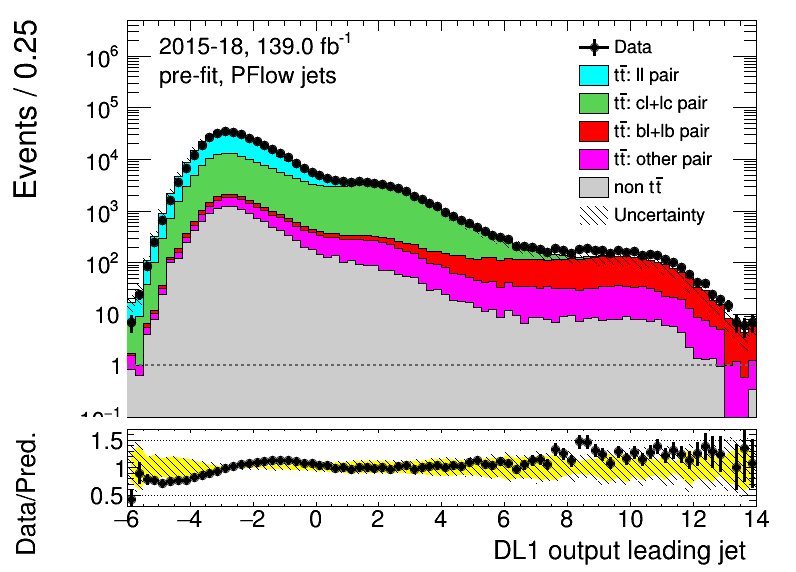
\includegraphics[width=.45\textwidth]{FTAG_plots/pretagNoRwwithhighpTPFlowall/DataMC_h_J0_DL1_log.png}
	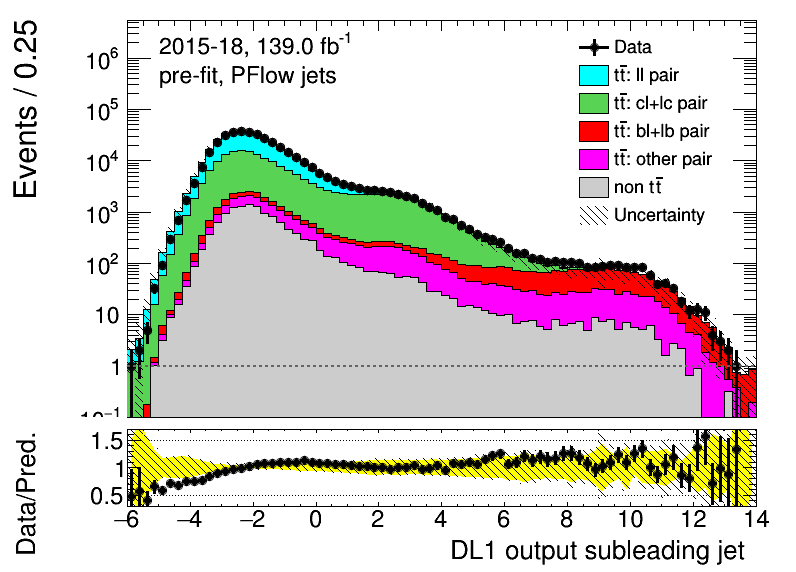
\includegraphics[width=.45\textwidth]{FTAG_plots/pretagNoRwwithhighpTPFlowall/DataMC_h_J1_DL1_log.png}\\
	\caption{DL1 tagger output}
	\end{subfigure}
	\begin{subfigure}[t]{1\linewidth}
		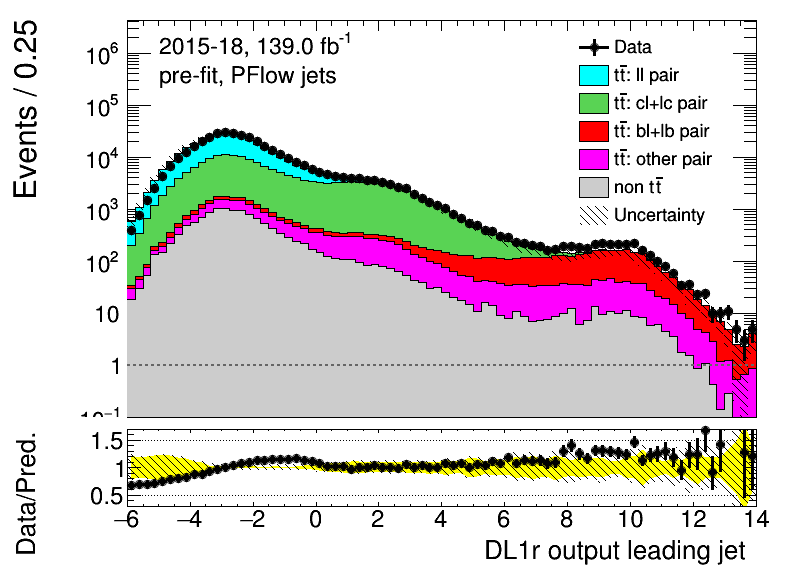
\includegraphics[width=.45\textwidth]{FTAG_plots/pretagNoRwwithhighpTPFlowall/DataMC_h_J0_DL1r_log.png}
		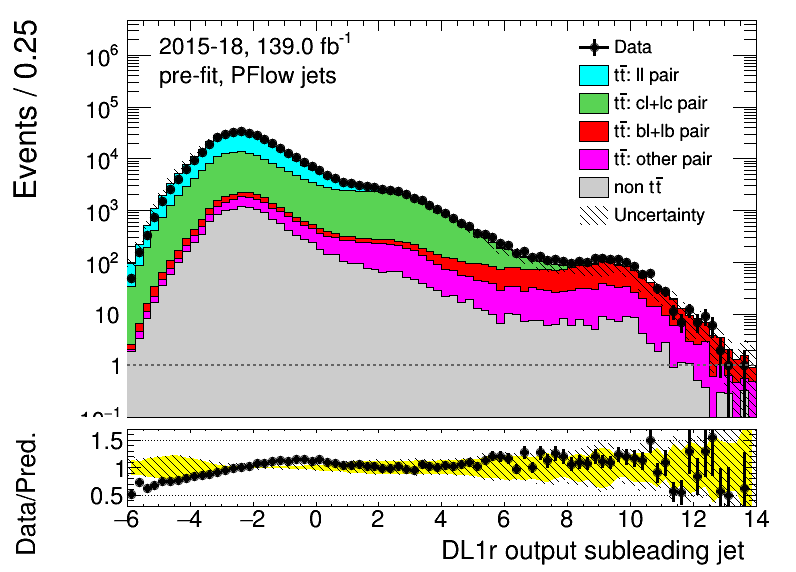
\includegraphics[width=.45\textwidth]{FTAG_plots/pretagNoRwwithhighpTPFlowall/DataMC_h_J1_DL1r_log.png}\\
		\caption{DL1r tagger output}
	\end{subfigure}
	\begin{subfigure}[t]{1\linewidth}
	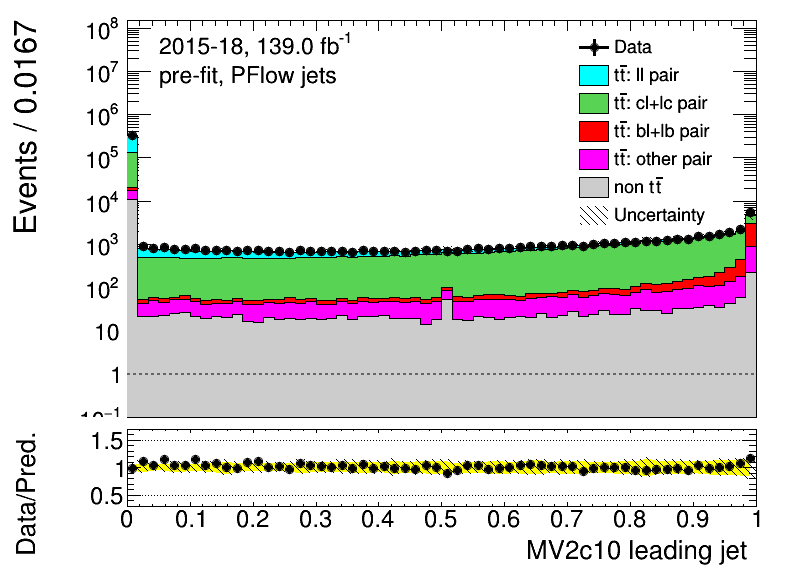
\includegraphics[width=.45\textwidth]{FTAG_plots/pretagNoRwwithhighpTPFlowall/DataMC_h_J0_MV2c10_log.png}
	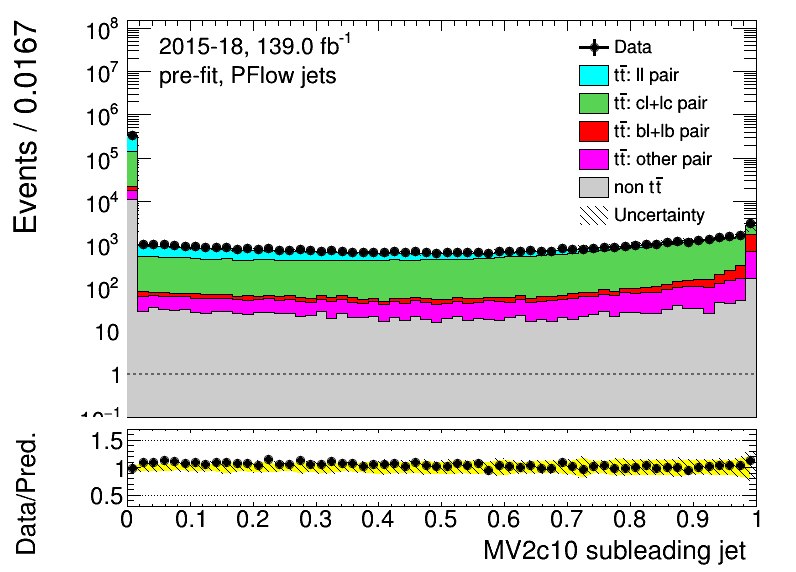
\includegraphics[width=.45\textwidth]{FTAG_plots/pretagNoRwwithhighpTPFlowall/DataMC_h_J1_MV2c10_log.png}\\
	\caption{MV2c10 tagger output}
	\end{subfigure}
	\caption{PFlow jets: distributions of the DL1, DL1r and MV2c10 
	tagger outputs of the combined selection, 
	leading jet in the left column and sub-leading jet in the right column,
	before fitting or tagging with full uncertainties.} \label{fig:taggers_PFlow}
\end{figure}
\newpage
\begin{figure}[H]
	\begin{subfigure}[t]{1\linewidth}
	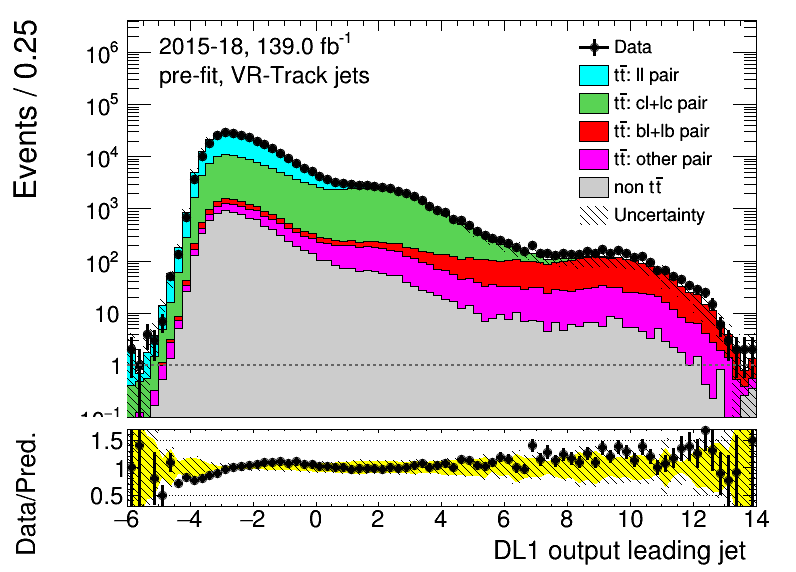
\includegraphics[width=.45\textwidth]{FTAG_plots/pretagNoRwwithhighpTVRJetsall/DataMC_h_J0_DL1trackjet_log.png}
	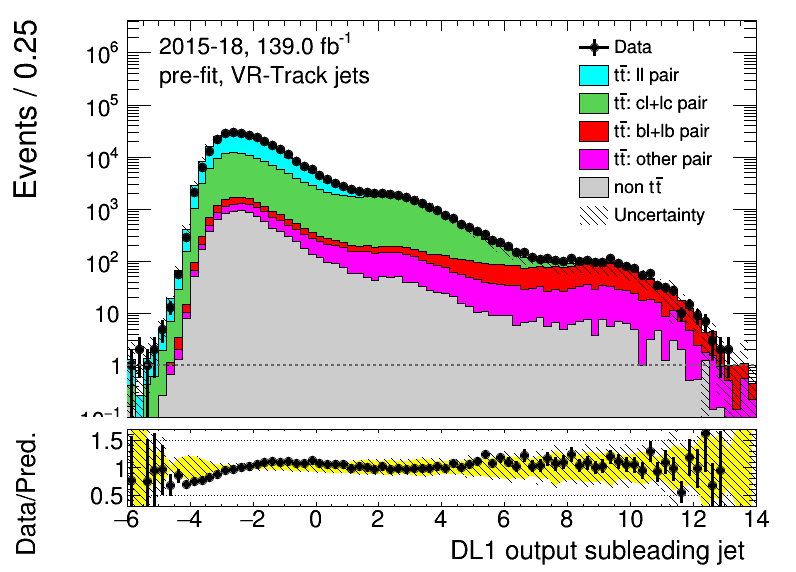
\includegraphics[width=.45\textwidth]{FTAG_plots/pretagNoRwwithhighpTVRJetsall/DataMC_h_J1_DL1trackjet_log.png}\\
	\caption{DL1 tagger output}
	\end{subfigure}
	\begin{subfigure}[t]{1\linewidth}
	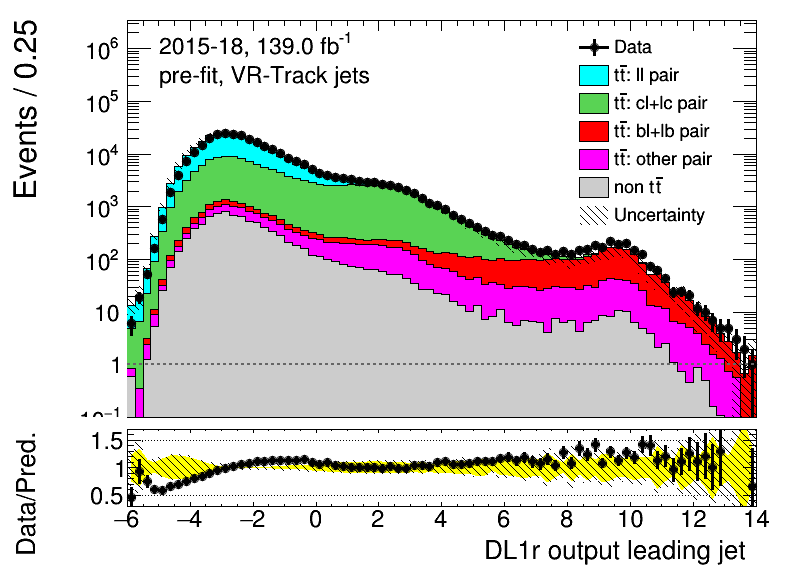
\includegraphics[width=.45\textwidth]{FTAG_plots/pretagNoRwwithhighpTVRJetsall/DataMC_h_J0_DL1rtrackjet_log.png}
	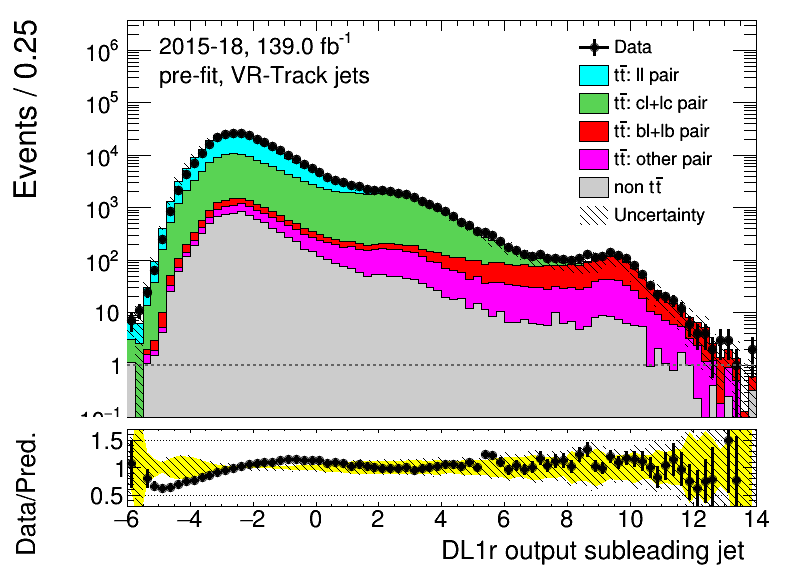
\includegraphics[width=.45\textwidth]{FTAG_plots/pretagNoRwwithhighpTVRJetsall/DataMC_h_J1_DL1rtrackjet_log.png}\\
	\caption{DL1r tagger output}
	\end{subfigure}
	\begin{subfigure}[t]{1\linewidth}
	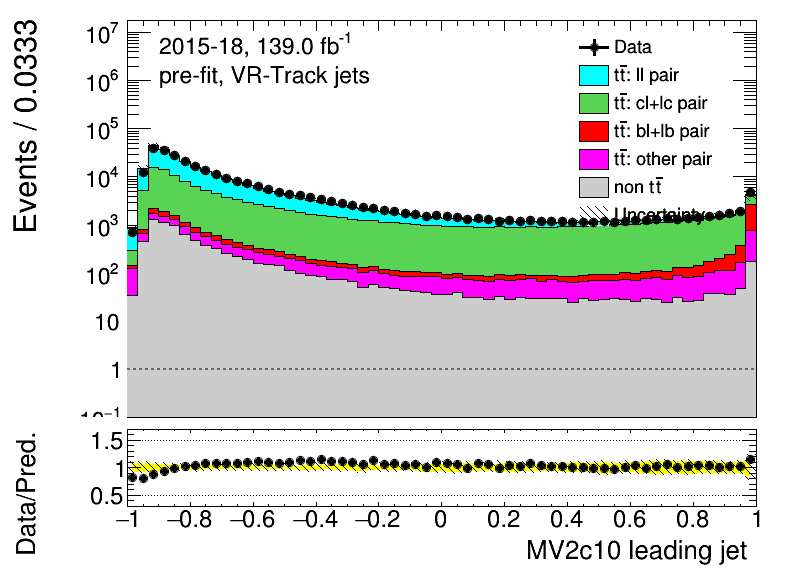
\includegraphics[width=.45\textwidth]{FTAG_plots/pretagNoRwwithhighpTVRJetsall/DataMC_h_J0_MV2c10_Fulltrackjet_log.png}
	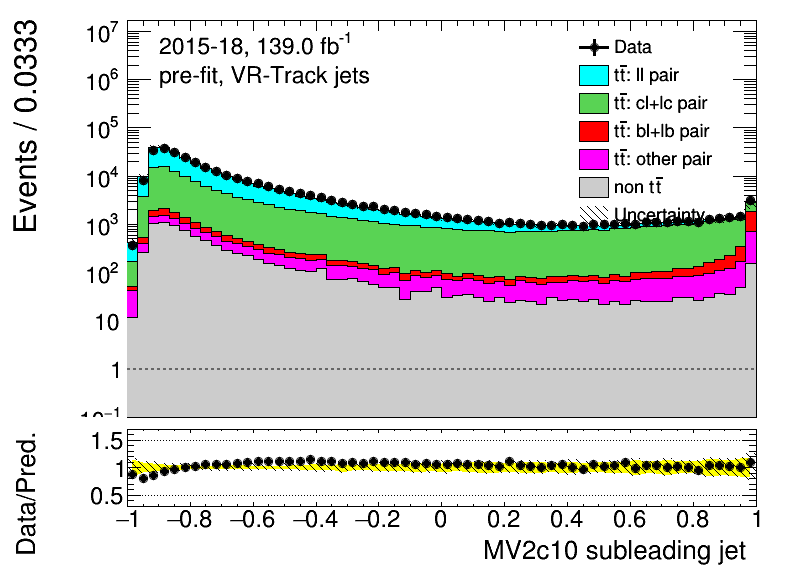
\includegraphics[width=.45\textwidth]{FTAG_plots/pretagNoRwwithhighpTVRJetsall/DataMC_h_J1_MV2c10_Fulltrackjet_log.png}\\
	\caption{MV2c10 tagger output}
	\end{subfigure}
	\caption{VR-Track jets: distributions of the DL1, DL1r and MV2c10 tagger outputs of 
	the combined selection, 
	leading jet in the left column and sub-leading jet in the right column,
	before fitting or tagging with full uncertainties.} \label{fig:taggers_VRJets}
\end{figure}	

\subsubsection{Efficiencies and Scale Factors}

%The Monte Carlo simulation demonstrates good agreement in different kinematic variables with data. 
The Dl1 and DL1r \cjet efficiencies and scale factors with systematics 
uncertainties are calculated with four fixed cut working points 
for the PFlow and VR VR-Track jets collection in the latest derivation 
in December 2020.

The \cjet\ mis-tagging efficiencies are shown in Figure \ref{fig:Dec_eff_PFlow_DL1}-\ref{fig:Dec_eff_VRJets_DL1r} 
for the PFlow jet collections and the VR-Track jets with the DL1 and the DL1r tagger. 
For PFlow jets, these results combine the standard selection, low\pt\ selection and the high-$p_T$ selection 
and for the VR-Track jets they combine the standard selection and the high-$p_T$ selection. 

The $1.25 \pm 0.25$ scale factor is applied on events with 3 true \bjets. 
The overall uncertainties are shown 
in the red band. 
The scale factors are shown in Figure \ref{fig:Dec_SF_PFlow_DL1}-\ref{fig:Dec_SF_VRJets_DL1r} for the PFlow jets
and the VR-Track jets with the DL1 and DL1r tagger. 
The tighter working points (60\%, 70\%) show larger uncertainties and bigger deviation from 1, while
the looser working points (77\%, 85\%) have much smaller uncertainty and the simulation is able to 
recover the data well due to more abundant events statistics.
For the PFlow jets, in most of the working points the systematic uncertainties dominate 
in the low-\pt\ bins (\pt\ < 150) and the statistical error, represented by the error bars on the 
markers, become more important in the last bin. 
For the VR-Track jets the statistical uncertainty is relatively constant for all bins while the 
systematic uncertainty increases as the \pt\ increases. 
To demonstrate the effect on statistics with the high-\pt\ selection, 
the fractional statistical uncertainties of 60\% working point scale factor
are shown in Table \ref{tab:stats_gain} for the standard and the combined selection.
In some bins the statistical uncertainty can decrease up to 30\%, suggesting that the
high-\pt\ selection is successful at increasing events statistics. 

\begin{table}[ht]
	\centering
	\small
	\setlength\tabcolsep{5pt} 
	\begin{tabular}{|r *2{|rr|r}| }
	\hline
	& \multicolumn{3}{|c|}{PFlow jets} & \multicolumn{3}{c|}{VR-Track jets} \\
	\hline
	&  \specialcell{Standard\\ selection} &\specialcell{ High-\pt\ \\selection }&\specialcell{ Fractional \\decrease} &  \specialcell{Standard\\ selection} &\specialcell{ High-\pt\ \\selection }&\specialcell{ Fractional \\decrease}\\
	\hline
	Bin No.1    &	 3.3\%  &3.3\% & 0.0\% & 5.6\%  & 5.3\%      &  5.7\%  \\
	Bin No.2    &    3.1\%  &2.8\% & 10.7\% & 4.2\%  & 3.7\%     & 13.5\%   \\
	Bin No.3    &    3.4\%  &2.6\% & 30.8\% & 5.8\%  & 4.9\%     & 18.4\%   \\
	Bin No.4    &    12.1\% &9.3\% & 30.1\% & 7.2\%  & 5.6\%     & 28.6\%   \\           
	\hline                 
	\end{tabular}
	\vspace{0.2cm}
	\caption{Comparison of the fractional statistical uncertainty in the DL1r 60\%
	working point scale factor. The \pt\ range of each bin can be found in section \ref{sec:Calibration method for charm jet}. }
	\label{tab:stats_gain}
	\end{table}



\newpage
%%% Efficiencies plots %%%

\begin{figure}[H]
	\centering
	\begin{subfigure}[t]{.35\linewidth}
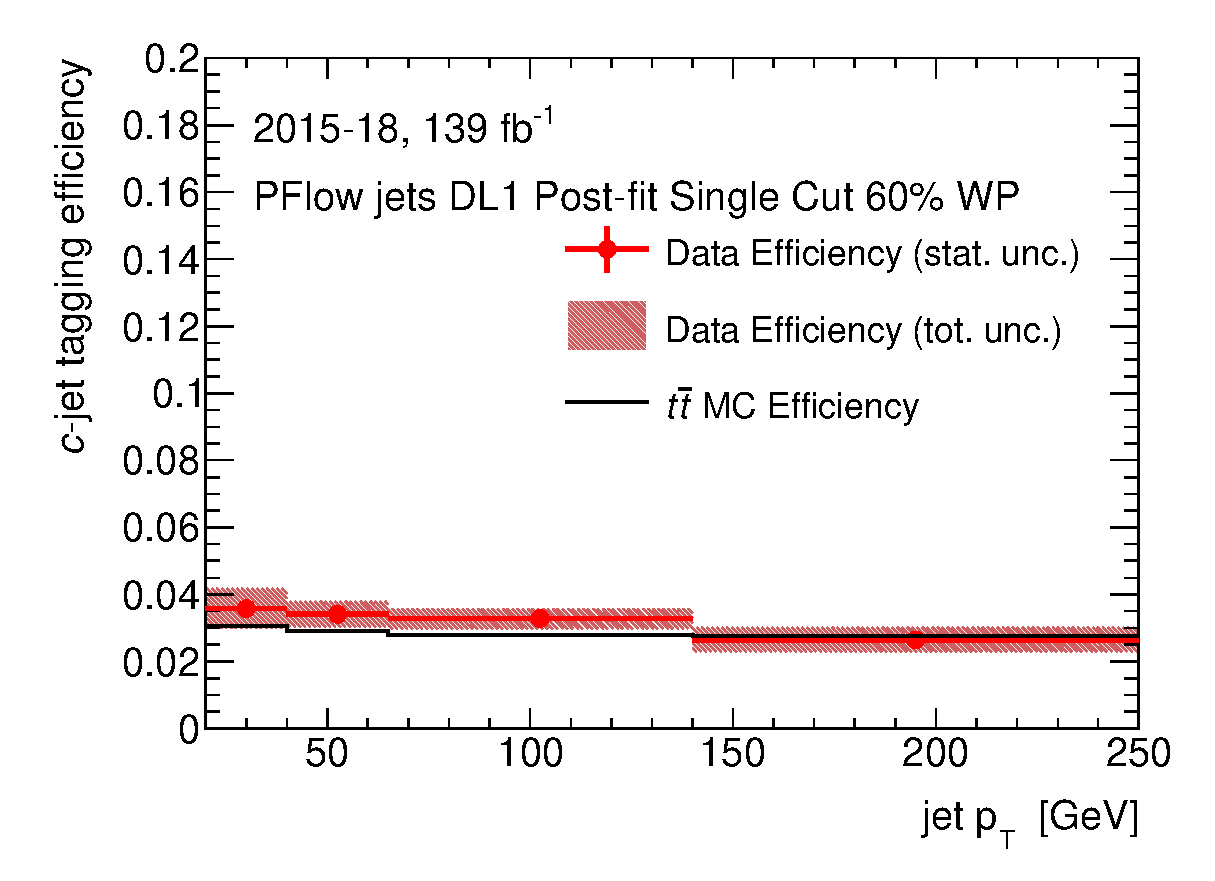
\includegraphics[width=1\textwidth]{FTAG_plots/DL1allPFlowDec/eff60.eps}
\caption{60\% working point}
	\end{subfigure}
\begin{subfigure}[t]{.35\linewidth}
	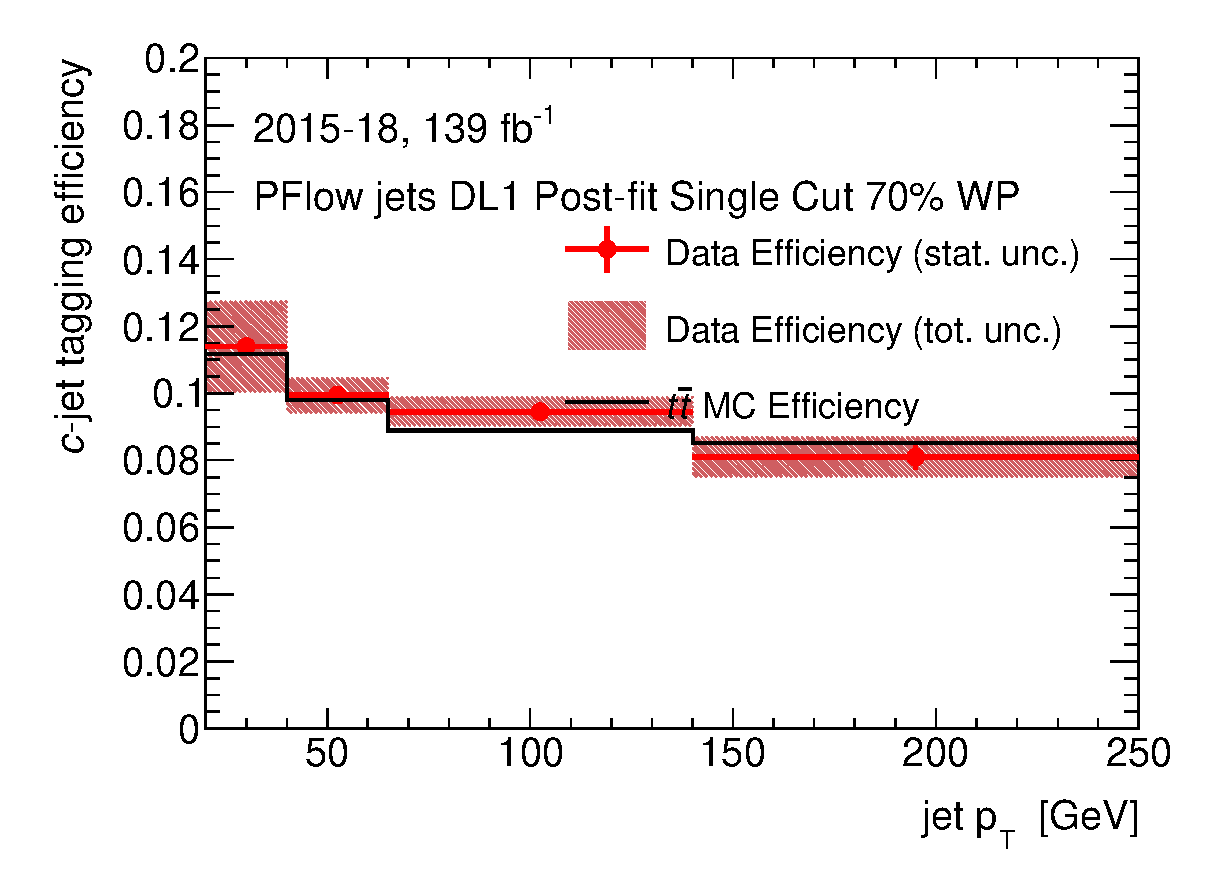
\includegraphics[width=1\textwidth]{FTAG_plots/DL1allPFlowDec/eff70.eps}
	\caption{70\% working point}
\end{subfigure}
\begin{subfigure}[t]{.35\linewidth}
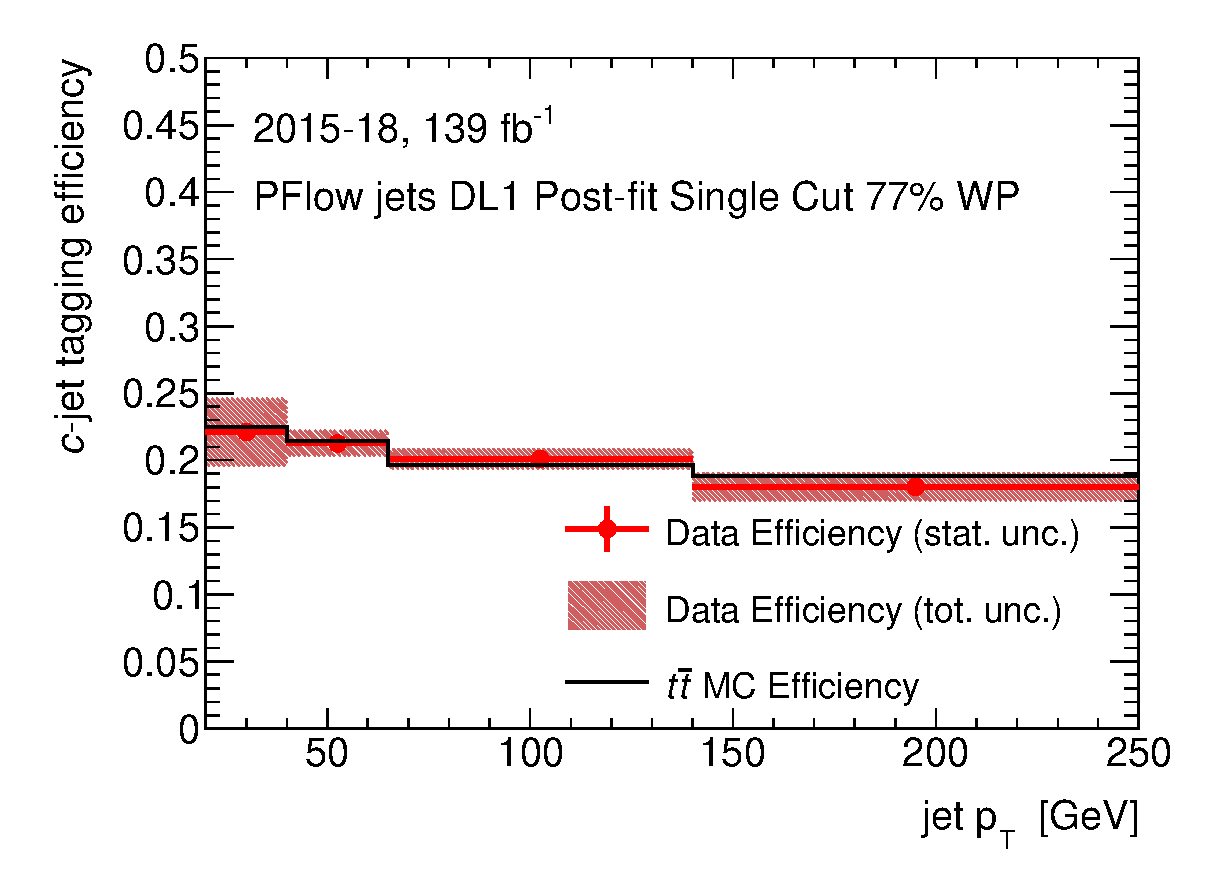
\includegraphics[width=1\textwidth]{FTAG_plots/DL1allPFlowDec/eff77.eps}
\caption{77\% working point}
\end{subfigure}
\begin{subfigure}[t]{.35\linewidth}
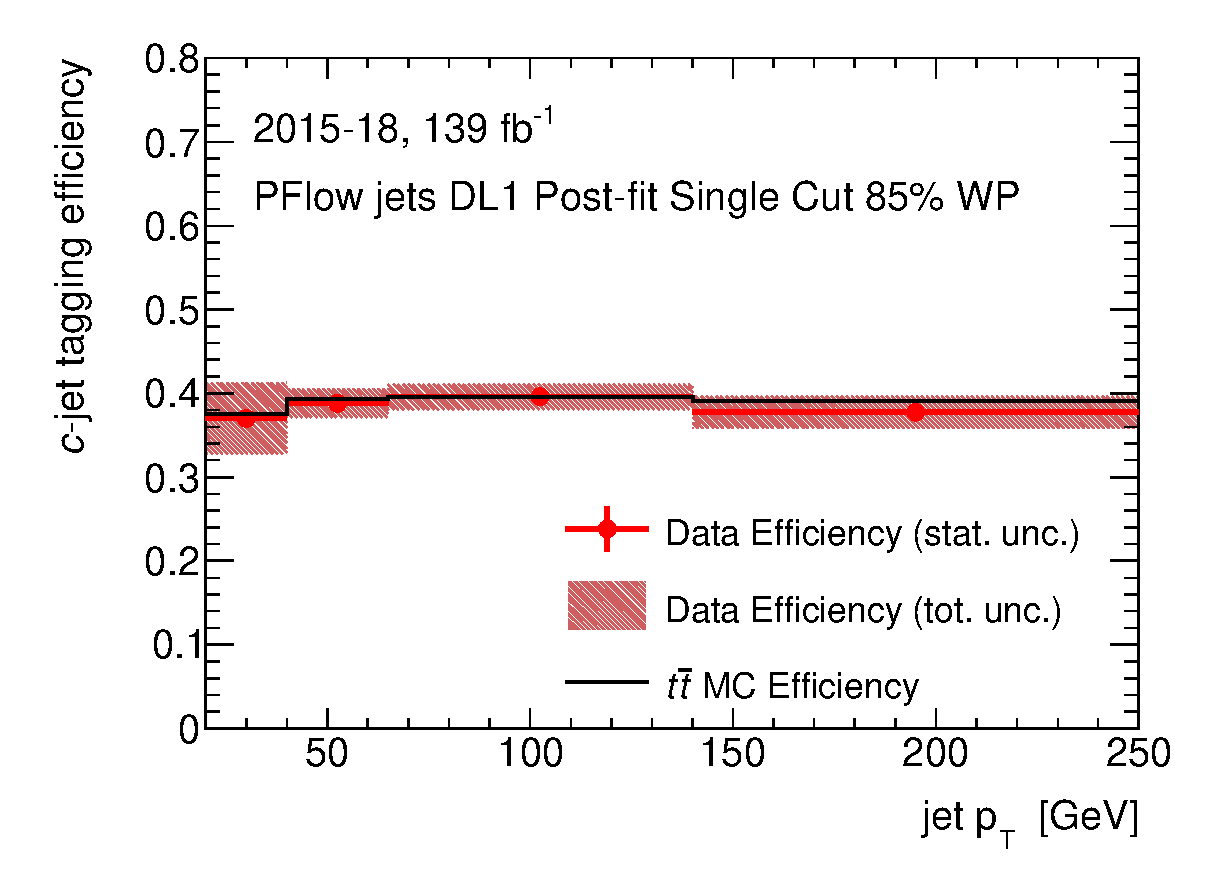
\includegraphics[width=1\textwidth]{FTAG_plots/DL1allPFlowDec/eff85.eps}
\caption{85\% working point}
\end{subfigure}
\caption{Charm-jet efficiencies for the PFlow jets collection with
the DL1 tagger.} \label{fig:Dec_eff_PFlow_DL1}
\end{figure}

\begin{figure}[H]
	\centering
	\begin{subfigure}[t]{.35\linewidth}
		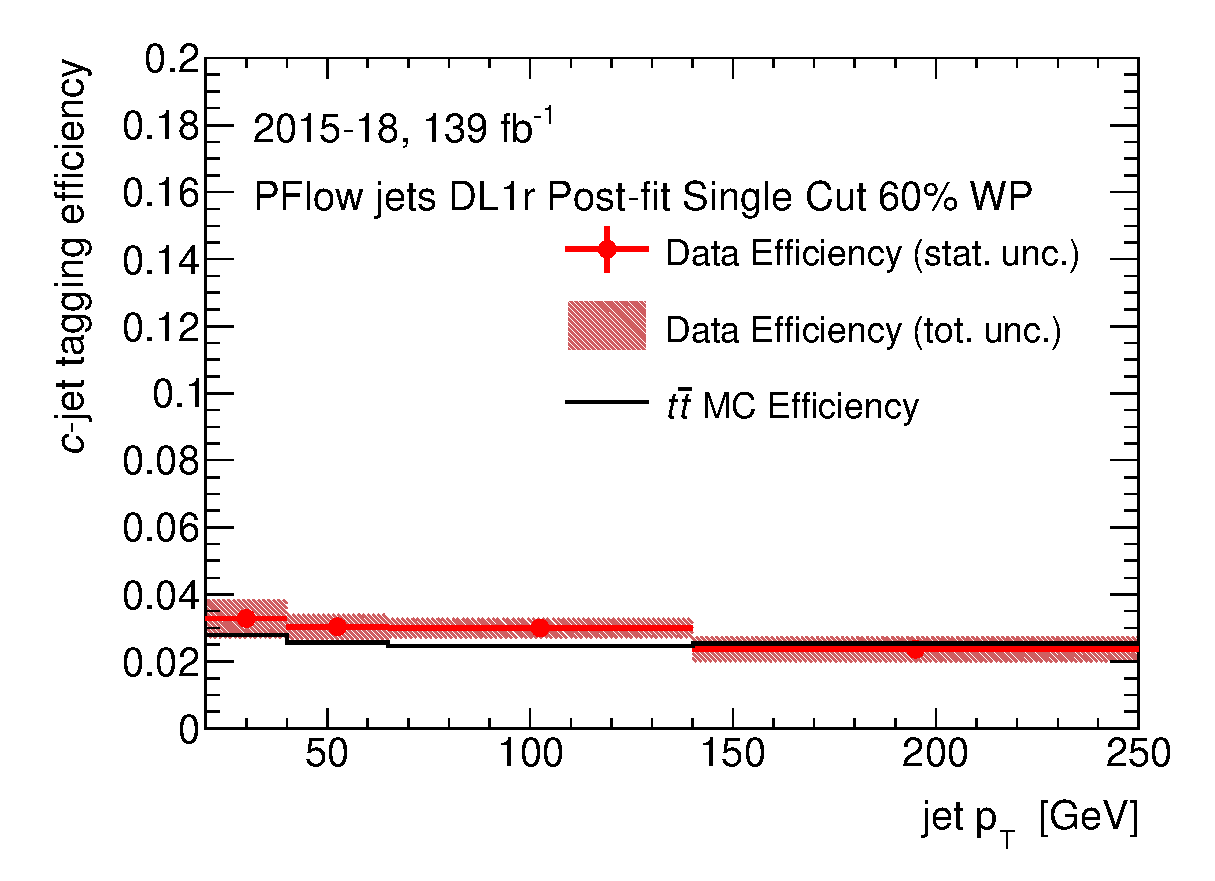
\includegraphics[width=1\textwidth]{FTAG_plots/DL1rallPFlowDec/eff60.eps}
		\caption{60\% working point}
			\end{subfigure}
		\begin{subfigure}[t]{.35\linewidth}
			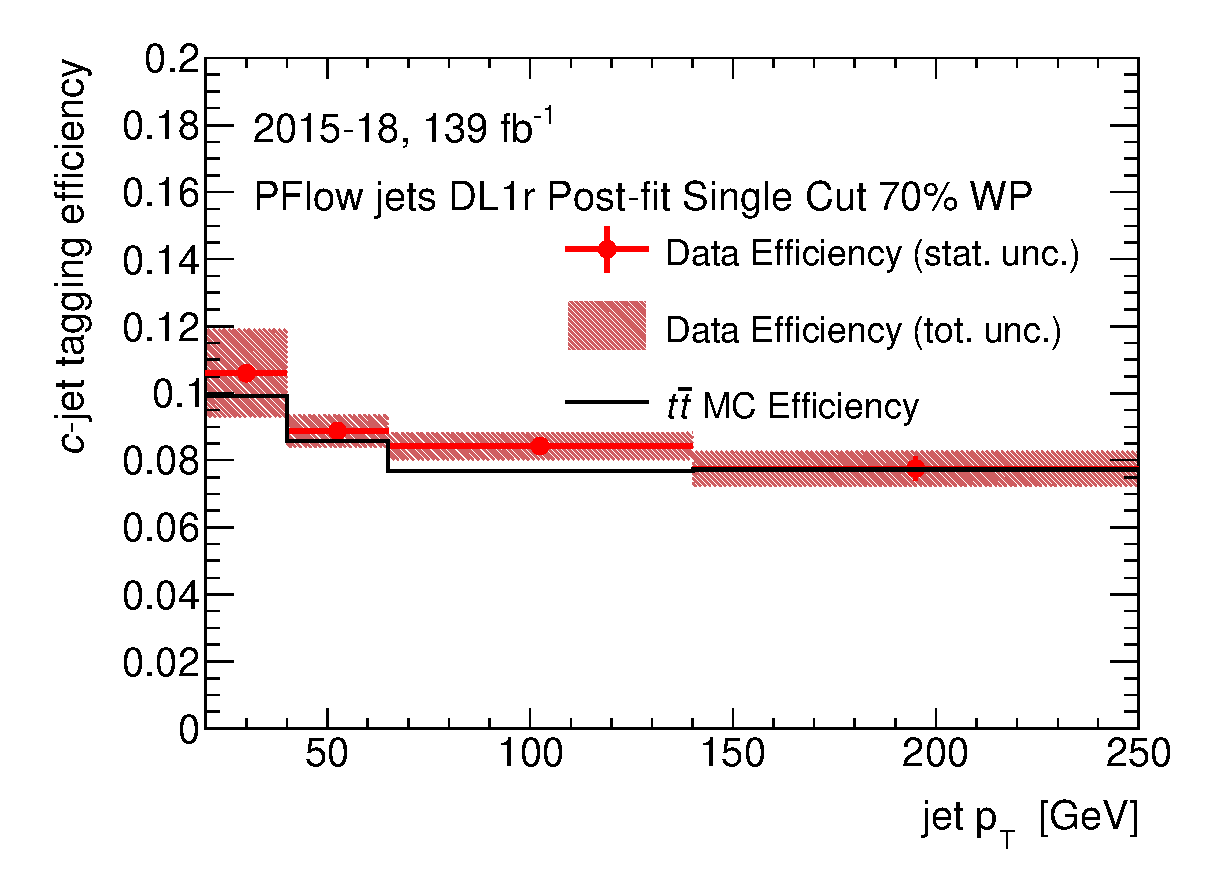
\includegraphics[width=1\textwidth]{FTAG_plots/DL1rallPFlowDec/eff70.eps}
			\caption{70\% working point}
		\end{subfigure}
		\begin{subfigure}[t]{.35\linewidth}
		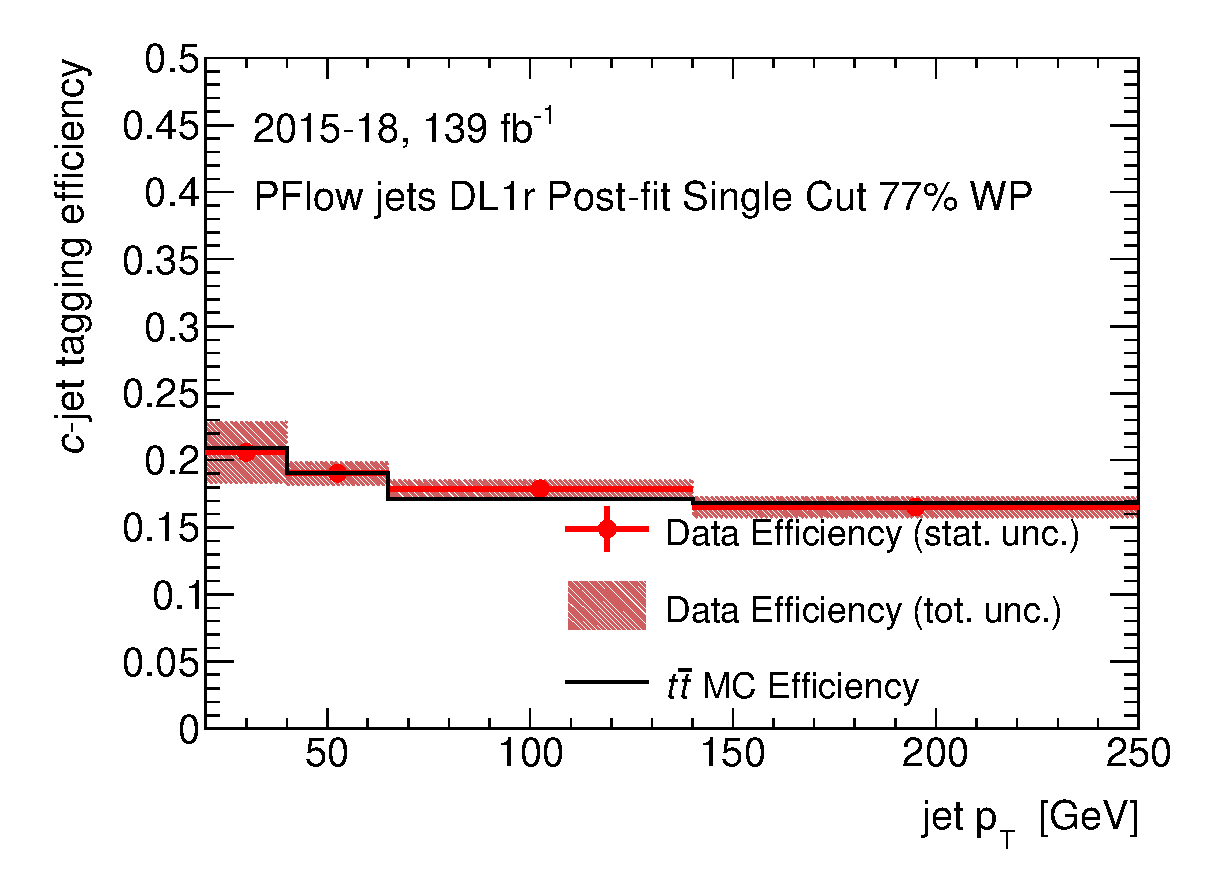
\includegraphics[width=1\textwidth]{FTAG_plots/DL1rallPFlowDec/eff77.eps}
		\caption{77\% working point}
		\end{subfigure}
		\begin{subfigure}[t]{.35\linewidth}
		\includegraphics[width=1\textwidth]{FTAG_plots/DL1rallPFlowDec/eff85.eps}
		\caption{85\% working point}
		\end{subfigure}
		\caption{Charm-jet efficiencies for the PFlow jets collection with
	the DL1r tagger.} \label{fig:Dec_eff_PFlow_DL1r}
\end{figure}


\newpage
\begin{figure}[H]
	\centering
	\begin{subfigure}[t]{.35\linewidth}
		\includegraphics[width=1\textwidth]{FTAG_plots/DL1allVRJetsDec/eff60.eps}
		\caption{60\% working point}
			\end{subfigure}
		\begin{subfigure}[t]{.35\linewidth}
			\includegraphics[width=1\textwidth]{FTAG_plots/DL1allVRJetsDec/eff70.eps}
			\caption{70\% working point}
		\end{subfigure}
		\begin{subfigure}[t]{.35\linewidth}
		\includegraphics[width=1\textwidth]{FTAG_plots/DL1allVRJetsDec/eff77.eps}
		\caption{77\% working point}
		\end{subfigure}
		\begin{subfigure}[t]{.35\linewidth}
		\includegraphics[width=1\textwidth]{FTAG_plots/DL1allVRJetsDec/eff85.eps}
		\caption{85\% working point}
		\end{subfigure}
	\caption{Charm-jet efficiencies for the VR-Track jets collection with
	the DL1 tagger.} \label{fig:Dec_eff_VRJets_DL1}
	\end{figure}

	\begin{figure}[H]
		\centering
		\begin{subfigure}[t]{.35\linewidth}
			\includegraphics[width=1\textwidth]{FTAG_plots/DL1rallVRJetsDec/eff60.eps}
			\caption{60\% working point}
				\end{subfigure}
			\begin{subfigure}[t]{.35\linewidth}
				\includegraphics[width=1\textwidth]{FTAG_plots/DL1rallVRJetsDec/eff70.eps}
				\caption{70\% working point}
			\end{subfigure}
			\begin{subfigure}[t]{.35\linewidth}
			\includegraphics[width=1\textwidth]{FTAG_plots/DL1rallVRJetsDec/eff77.eps}
			\caption{77\% working point}
			\end{subfigure}
			\begin{subfigure}[t]{.35\linewidth}
			\includegraphics[width=1\textwidth]{FTAG_plots/DL1rallVRJetsDec/eff85.eps}
			\caption{85\% working point}
			\end{subfigure}
		\caption{Charm-jet efficiencies for the VR-Track jets collection with
		the DL1r tagger.} \label{fig:Dec_eff_VRJets_DL1r}
\end{figure}

\newpage
%SF plots
\begin{figure}[H]
	\centering
	\begin{subfigure}[t]{.35\linewidth}
		\includegraphics[width=1\textwidth]{FTAG_plots/DL1allPFlowDec/SF60.eps}
		\caption{60\% working point}
			\end{subfigure}
		\begin{subfigure}[t]{.35\linewidth}
			\includegraphics[width=1\textwidth]{FTAG_plots/DL1allPFlowDec/SF70.eps}
			\caption{70\% working point}
		\end{subfigure}
		\begin{subfigure}[t]{.35\linewidth}
		\includegraphics[width=1\textwidth]{FTAG_plots/DL1allPFlowDec/SF77.eps}
		\caption{77\% working point}
		\end{subfigure}
		\begin{subfigure}[t]{.35\linewidth}
		\includegraphics[width=1\textwidth]{FTAG_plots/DL1allPFlowDec/SF85.eps}
		\caption{85\% working point}
		\end{subfigure}
	\caption{Charm-jet scale factors for the PFlow jets collection with 
	the DL1 tagger.} \label{fig:Dec_SF_PFlow_DL1}
	\end{figure}
	

\begin{figure}[H]
	\centering
	\begin{subfigure}[t]{.35\linewidth}
		\includegraphics[width=1\textwidth]{FTAG_plots/DL1rallPFlowDec/SF60.eps}
		\caption{60\% working point}
			\end{subfigure}
		\begin{subfigure}[t]{.35\linewidth}
			\includegraphics[width=1\textwidth]{FTAG_plots/DL1rallPFlowDec/SF70.eps}
			\caption{70\% working point}
		\end{subfigure}
		\begin{subfigure}[t]{.35\linewidth}
		\includegraphics[width=1\textwidth]{FTAG_plots/DL1rallPFlowDec/SF77.eps}
		\caption{77\% working point}
		\end{subfigure}
		\begin{subfigure}[t]{.35\linewidth}
		\includegraphics[width=1\textwidth]{FTAG_plots/DL1rallPFlowDec/SF85.eps}
		\caption{85\% working point}
		\end{subfigure}
	\caption{Charm-jet scale factors for the PFlow jets collection with 
	the DL1r tagger.} \label{fig:Dec_SF_PFlow_DL1r}
	\end{figure}	
\newpage
\begin{figure}[H]
	\centering
	\begin{subfigure}[t]{.35\linewidth}
		\includegraphics[width=1\textwidth]{FTAG_plots/DL1allVRJetsDec/SF60.eps}
		\caption{60\% working point}
			\end{subfigure}
		\begin{subfigure}[t]{.35\linewidth}
			\includegraphics[width=1\textwidth]{FTAG_plots/DL1allVRJetsDec/SF70.eps}
			\caption{70\% working point}
		\end{subfigure}
		\begin{subfigure}[t]{.35\linewidth}
		\includegraphics[width=1\textwidth]{FTAG_plots/DL1allVRJetsDec/SF77.eps}
		\caption{77\% working point}
		\end{subfigure}
		\begin{subfigure}[t]{.35\linewidth}
		\includegraphics[width=1\textwidth]{FTAG_plots/DL1allVRJetsDec/SF85.eps}
		\caption{85\% working point}
		\end{subfigure}
	\caption{Charm-jet scale factors for the VR-Track jets collection with 
	the DL1 tagger.} \label{fig:Dec_SF_VRJets_DL1}
	\end{figure}
	

\begin{figure}[H]
	\centering
	\begin{subfigure}[t]{.35\linewidth}
		\includegraphics[width=1\textwidth]{FTAG_plots/DL1rallVRJetsDec/SF60.eps}
		\caption{60\% working point}
			\end{subfigure}
		\begin{subfigure}[t]{.35\linewidth}
			\includegraphics[width=1\textwidth]{FTAG_plots/DL1rallVRJetsDec/SF70.eps}
			\caption{70\% working point}
		\end{subfigure}
		\begin{subfigure}[t]{.35\linewidth}
		\includegraphics[width=1\textwidth]{FTAG_plots/DL1rallVRJetsDec/SF77.eps}
		\caption{77\% working point}
		\end{subfigure}
		\begin{subfigure}[t]{.35\linewidth}
		\includegraphics[width=1\textwidth]{FTAG_plots/DL1rallVRJetsDec/SF85.eps}
		\caption{85\% working point}
		\end{subfigure}
	\caption{Charm-jet scale factors for the VR-Track jets collection with 
	the DL1r tagger.} \label{fig:Dec_SF_VRJets_DL1r}
	\end{figure}	


\newpage
\iffalse


In terms of statistical gain, taking the 60\% working point scale factor with 2018 data as an example, the error is reduced as expected. In the last bin of the $p_{T}$ distribution of scale factors, the error is reduced by 55\%, which suggests the success of high-$p_{T}$ selection method. The percentage reduction of error of each bin is given in Tab.\ref{tab:limit}:


 \begin{table}[ht]
 \begin{centering}
 \begin{tabular}{|p{2.5em}||p{2.5em}|p{2.5em}|p{5em}||p{2.5em}|p{2.5em}|p{5em}||p{5em}|}
          \hline
          & \multicolumn{3}{|c||}{high-$p_{T}$ + standard selection} & \multicolumn{3}{|c||}{standard selection only} & \\  \hline\hline
          Bins& Bin Value &Bin error&Percentage error&Bin Value &Bin error&Percentage error & Error reduction\\ \hline
          Bin 1 & 1.25 & 0.12 & 10\% &1.20 & 0.13 & 11\% & 11\% \\ \hline
          Bin 2 & 1.34 & 0.10 & 8\% & 1.24 & 0.11 & 9\% & 18\% \\ \hline
          Bin 3 & 1.22 & 0.10 & 8\% & 1.04 & 0.11 & 10\% & 28\% \\ \hline
          Bin 4 & 0.98 & 0.24 & 24\% & 0.72 & 0.27 & 37\% & 55\% \\ \hline
          
 
 \end{tabular} 
 \caption{Bins values and the corresponding errors of the scale factor at 60\% working point, with 2018 data.}
 \end{centering}
 \label{tab:limit}
 \end{table}

\fi

\newpage




\section{Search for Higgs boson pair production in the \bbtt\ channel}
\label{sec:search for dihiggs}
\subsection{Data and Monte Carlo samples}
\subsection{Trigger and event selection}
\subsection{Background estimation}
\subsection{Multivariate analysis}
\subsection{Systematic uncertainties}
\subsection{Results}




\section{Summary}





\newpage
\newpage
\printbibliography


\appendix
\newpage


\section{Supplementary material for \cjet\ calibration}
\subsection{Additional plots for kinematic variables}
\subsubsection{Standard selection}

\label{sec:appendix_standard_selection}
\newpage	
\begin{figure}[H]
\includegraphics[width=.45\textwidth]{FTAG_plots/pretagNoRwwithouthighpTPFlowall/DataMC_h_J0_eta.png}
\includegraphics[width=.45\textwidth]{FTAG_plots/pretagNoRwwithouthighpTPFlowall/DataMC_h_J1_eta.png}\\
\includegraphics[width=.45\textwidth]{FTAG_plots/pretagNoRwwithouthighpTPFlowall/DataMC_h_LLR.png}
\includegraphics[width=.45\textwidth]{FTAG_plots/pretagNoRwwithouthighpTPFlowall/DataMC_h_MET.png}\\

\caption{PFlow jets: distributions of the leading and sub-leading jets 
from W decay, KLFitter output and the transverse missing transverse 
energy of the standard selection, before fitting or tagging with 
full uncertainties.} \label{fig:standard_jets_PFlow}
\end{figure}

\newpage
\begin{figure}[H]
\includegraphics[width=.45\textwidth]{FTAG_plots/pretagNoRwwithouthighpTPFlowall/DataMC_h_dRbb.png}
\includegraphics[width=.45\textwidth]{FTAG_plots/pretagNoRwwithouthighpTPFlowall/DataMC_h_dRqq.png}\\
\includegraphics[width=.45\textwidth]{FTAG_plots/pretagNoRwwithouthighpTPFlowall/DataMC_h_dRbhadq1.png}
\includegraphics[width=.45\textwidth]{FTAG_plots/pretagNoRwwithouthighpTPFlowall/DataMC_h_dRblepq1.png} \\
\includegraphics[width=.45\textwidth]{FTAG_plots/pretagNoRwwithouthighpTPFlowall/DataMC_h_dRWhadbhad.png} 
\includegraphics[width=.45\textwidth]{FTAG_plots/pretagNoRwwithouthighpTPFlowall/DataMC_h_dRWhadblep.png} \\
\caption{PFlow jets: distributions of angle related variables of the combination of the standard selection,
 before fitting or 
tagging with full uncertainties.} \label{fig:standard_angles_PFlow}
\end{figure}

\newpage
\begin{figure}[H]
\includegraphics[width=.45\textwidth]{FTAG_plots/pretagNoRwwithouthighpTPFlowall/DataMC_h_Mbb.png}
\includegraphics[width=.45\textwidth]{FTAG_plots/pretagNoRwwithouthighpTPFlowall/DataMC_h_mjj.png}\\
\includegraphics[width=.45\textwidth]{FTAG_plots/pretagNoRwwithouthighpTPFlowall/DataMC_h_mjjj.png}
\includegraphics[width=.45\textwidth]{FTAG_plots/pretagNoRwwithouthighpTPFlowall/DataMC_h_Htjj.png}\\
\caption{PFlow jets: distributions of mass related variables of the standard selection, 
before fitting or 
tagging with stat-only uncertainties.} \label{fig:standard_mass_PFlow}
\end{figure}



\newpage	
\begin{figure}[H]
\includegraphics[width=.45\textwidth]{FTAG_plots/pretagNoRwwithouthighpTVRJetsall/DataMC_h_J0_etatrackjet.png}
\includegraphics[width=.45\textwidth]{FTAG_plots/pretagNoRwwithouthighpTVRJetsall/DataMC_h_J1_etatrackjet.png}\\
\includegraphics[width=.45\textwidth]{FTAG_plots/pretagNoRwwithouthighpTVRJetsall/DataMC_h_LLRtrackjet.png}
\includegraphics[width=.45\textwidth]{FTAG_plots/pretagNoRwwithouthighpTVRJetsall/DataMC_h_METtrackjet.png}\\

\caption{VR-Track jets: distributions of the leading and sub-leading jets 
from W decay, KLFitter output and the transverse missing transverse 
energy of the standard selection, before fitting or tagging with 
full uncertainties.} \label{fig:standard_jets_VRJets}
\end{figure}



\newpage
\begin{figure}[H]
\includegraphics[width=.45\textwidth]{FTAG_plots/pretagNoRwwithouthighpTVRJetsall/DataMC_h_dRbbtrackjet.png}
\includegraphics[width=.45\textwidth]{FTAG_plots/pretagNoRwwithouthighpTVRJetsall/DataMC_h_dRqqtrackjet.png}\\
\includegraphics[width=.45\textwidth]{FTAG_plots/pretagNoRwwithouthighpTVRJetsall/DataMC_h_dRbhadq1trackjet.png}
\includegraphics[width=.45\textwidth]{FTAG_plots/pretagNoRwwithouthighpTVRJetsall/DataMC_h_dRblepq1trackjet.png} \\
\includegraphics[width=.45\textwidth]{FTAG_plots/pretagNoRwwithouthighpTVRJetsall/DataMC_h_dRWhadbhadtrackjet.png} 
\includegraphics[width=.45\textwidth]{FTAG_plots/pretagNoRwwithouthighpTVRJetsall/DataMC_h_dRWhadbleptrackjet.png} \\
\caption{VR-Track jets: distributions of angle related variables of the combination 
of the standard selection, before fitting or tagging with full uncertainties.} \label{fig:standard_angles_VRJets}
\end{figure}

\newpage
\begin{figure}[H]
\includegraphics[width=.45\textwidth]{FTAG_plots/pretagNoRwwithouthighpTVRJetsall/DataMC_h_Mbbtrackjet.png}
\includegraphics[width=.45\textwidth]{FTAG_plots/pretagNoRwwithouthighpTVRJetsall/DataMC_h_mjjtrackjet.png}\\
\includegraphics[width=.45\textwidth]{FTAG_plots/pretagNoRwwithouthighpTVRJetsall/DataMC_h_mjjjtrackjet.png}
\includegraphics[width=.45\textwidth]{FTAG_plots/pretagNoRwwithouthighpTVRJetsall/DataMC_h_Htjjtrackjet.png}\\
\caption{VR-Track jets: distributions of mass related variables of the standard selection, 
before fitting or tagging with stat-only uncertainties.} \label{fig:standard_mass_VRJets}
\end{figure}


\subsubsection{Low-\pt\ selection}
\label{sec:appendix_lowpT_selection}
\newpage	
\begin{figure}[H]
\includegraphics[width=.45\textwidth]{FTAG_plots/pretagNoRwLowpTPFlowall/DataMC_h_J0_eta.png}
\includegraphics[width=.45\textwidth]{FTAG_plots/pretagNoRwLowpTPFlowall/DataMC_h_J1_eta.png}\\
\includegraphics[width=.45\textwidth]{FTAG_plots/pretagNoRwLowpTPFlowall/DataMC_h_LLR.png}
\includegraphics[width=.45\textwidth]{FTAG_plots/pretagNoRwLowpTPFlowall/DataMC_h_MET.png}\\

\caption{PFlow jets: distributions of the leading and sub-leading jets 
from W decay, KLFitter output and the transverse missing transverse 
energy of the low-\pt\ selection, before fitting or tagging with 
full uncertainties.} \label{fig:lowpT_jets_VRJets}
\end{figure}

\newpage
\begin{figure}[H]
\includegraphics[width=.45\textwidth]{FTAG_plots/pretagNoRwLowpTPFlowall/DataMC_h_dRbb.png}
\includegraphics[width=.45\textwidth]{FTAG_plots/pretagNoRwLowpTPFlowall/DataMC_h_dRqq.png}\\
\includegraphics[width=.45\textwidth]{FTAG_plots/pretagNoRwLowpTPFlowall/DataMC_h_dRbhadq1.png}
\includegraphics[width=.45\textwidth]{FTAG_plots/pretagNoRwLowpTPFlowall/DataMC_h_dRblepq1.png} \\
\includegraphics[width=.45\textwidth]{FTAG_plots/pretagNoRwLowpTPFlowall/DataMC_h_dRWhadbhad.png} 
\includegraphics[width=.45\textwidth]{FTAG_plots/pretagNoRwLowpTPFlowall/DataMC_h_dRWhadblep.png} \\
\caption{PFlow jets: distributions of angle related variables of the combination of the low-\pt\ selection,
 before fitting or 
tagging with full uncertainties.} \label{fig:lowpT_angles_PFlow}
\end{figure}

\newpage
\begin{figure}[H]
\includegraphics[width=.45\textwidth]{FTAG_plots/pretagNoRwLowpTPFlowall/DataMC_h_Mbb.png}
\includegraphics[width=.45\textwidth]{FTAG_plots/pretagNoRwLowpTPFlowall/DataMC_h_mjj.png}\\
\includegraphics[width=.45\textwidth]{FTAG_plots/pretagNoRwLowpTPFlowall/DataMC_h_mjjj.png}
\includegraphics[width=.45\textwidth]{FTAG_plots/pretagNoRwLowpTPFlowall/DataMC_h_Htjj.png}\\
\caption{PFlow jets: distributions of mass related variables of the low-\pt\ selection, 
before fitting or 
tagging with stat-only uncertainties.} \label{fig:lowpT_mass_PFlow}
\end{figure}

\subsection{High-\pt\ selection}
\label{sec:appendix_highpT_selection}
\newpage	
\begin{figure}[H]
\includegraphics[width=.45\textwidth]{FTAG_plots/pretagNoRwnewonlyPFlowall/DataMC_h_J0_eta.png}
\includegraphics[width=.45\textwidth]{FTAG_plots/pretagNoRwnewonlyPFlowall/DataMC_h_J1_eta.png}\\
\includegraphics[width=.45\textwidth]{FTAG_plots/pretagNoRwnewonlyPFlowall/DataMC_h_LLR.png}
\includegraphics[width=.45\textwidth]{FTAG_plots/pretagNoRwnewonlyPFlowall/DataMC_h_MET.png}\\

\caption{PFlow jets: distributions of the leading and sub-leading jets 
from W decay, KLFitter output and the transverse missing transverse 
energy of the high-\pt\ selection, before fitting or tagging with 
full uncertainties.} \label{fig:highpT_jets_PFlow}
\end{figure}

\newpage
\begin{figure}[H]
\includegraphics[width=.45\textwidth]{FTAG_plots/pretagNoRwnewonlyPFlowall/DataMC_h_dRbb.png}
\includegraphics[width=.45\textwidth]{FTAG_plots/pretagNoRwnewonlyPFlowall/DataMC_h_dRqq.png}\\
\includegraphics[width=.45\textwidth]{FTAG_plots/pretagNoRwnewonlyPFlowall/DataMC_h_dRbhadq1.png}
\includegraphics[width=.45\textwidth]{FTAG_plots/pretagNoRwnewonlyPFlowall/DataMC_h_dRblepq1.png} \\
\includegraphics[width=.45\textwidth]{FTAG_plots/pretagNoRwnewonlyPFlowall/DataMC_h_dRWhadbhad.png} 
\includegraphics[width=.45\textwidth]{FTAG_plots/pretagNoRwnewonlyPFlowall/DataMC_h_dRWhadblep.png} \\
\caption{PFlow jets: distributions of angle related variables of the combination of the high-\pt\ selection,
 before fitting or 
tagging with full uncertainties.} \label{fig:highpT_angles_PFlow}
\end{figure}

\newpage
\begin{figure}[H]
\includegraphics[width=.45\textwidth]{FTAG_plots/pretagNoRwnewonlyPFlowall/DataMC_h_Mbb.png}
\includegraphics[width=.45\textwidth]{FTAG_plots/pretagNoRwnewonlyPFlowall/DataMC_h_mjj.png}\\
\includegraphics[width=.45\textwidth]{FTAG_plots/pretagNoRwnewonlyPFlowall/DataMC_h_mjjj.png}
\includegraphics[width=.45\textwidth]{FTAG_plots/pretagNoRwnewonlyPFlowall/DataMC_h_Htjj.png}\\
\caption{PFlow jets: distributions of mass related variables of the high-\pt\ selection, 
before fitting or 
tagging with stat-only uncertainties.} \label{fig:highpT_mass_PFlow}
\end{figure}



\newpage	
\begin{figure}[H]
\includegraphics[width=.45\textwidth]{FTAG_plots/pretagNoRwnewonlyVRJetsall/DataMC_h_J0_etatrackjet.png}
\includegraphics[width=.45\textwidth]{FTAG_plots/pretagNoRwnewonlyVRJetsall/DataMC_h_J1_etatrackjet.png}\\
\includegraphics[width=.45\textwidth]{FTAG_plots/pretagNoRwnewonlyVRJetsall/DataMC_h_LLRtrackjet.png}
\includegraphics[width=.45\textwidth]{FTAG_plots/pretagNoRwnewonlyVRJetsall/DataMC_h_METtrackjet.png}\\

\caption{VR-Track jets: distributions of the leading and sub-leading jets 
from W decay, KLFitter output and the transverse missing transverse 
energy of the high-\pt\ selection, before fitting or tagging with 
full uncertainties.} \label{fig:highpT_jets_VRJets}
\end{figure}



\newpage
\begin{figure}[H]
\includegraphics[width=.45\textwidth]{FTAG_plots/pretagNoRwnewonlyVRJetsall/DataMC_h_dRbbtrackjet.png}
\includegraphics[width=.45\textwidth]{FTAG_plots/pretagNoRwnewonlyVRJetsall/DataMC_h_dRqqtrackjet.png}\\
\includegraphics[width=.45\textwidth]{FTAG_plots/pretagNoRwnewonlyVRJetsall/DataMC_h_dRbhadq1trackjet.png}
\includegraphics[width=.45\textwidth]{FTAG_plots/pretagNoRwnewonlyVRJetsall/DataMC_h_dRblepq1trackjet.png} \\
\includegraphics[width=.45\textwidth]{FTAG_plots/pretagNoRwnewonlyVRJetsall/DataMC_h_dRWhadbhadtrackjet.png} 
\includegraphics[width=.45\textwidth]{FTAG_plots/pretagNoRwnewonlyVRJetsall/DataMC_h_dRWhadbleptrackjet.png} \\
\caption{VR-Track jets: distributions of angle related variables of the combination 
of the high-\pt\ selection, before fitting or tagging with full uncertainties.} \label{fig:highpT_angles_VRJets}
\end{figure}

\newpage
\begin{figure}[H]
\includegraphics[width=.45\textwidth]{FTAG_plots/pretagNoRwnewonlyVRJetsall/DataMC_h_Mbbtrackjet.png}
\includegraphics[width=.45\textwidth]{FTAG_plots/pretagNoRwnewonlyVRJetsall/DataMC_h_mjjtrackjet.png}\\
\includegraphics[width=.45\textwidth]{FTAG_plots/pretagNoRwnewonlyVRJetsall/DataMC_h_mjjjtrackjet.png}
\includegraphics[width=.45\textwidth]{FTAG_plots/pretagNoRwnewonlyVRJetsall/DataMC_h_Htjjtrackjet.png}\\
\caption{VR-Track jets: distributions of mass related variables of the high-\pt\ selection, 
before fitting or tagging with stat-only uncertainties.} \label{fig:highpT_mass_VRJets}
\end{figure}


	

	\newpage
	\subsection{Combined selection}
	\label{sec:appendix_combined_selection}
	\newpage	
	\begin{figure}[H]
	\includegraphics[width=.45\textwidth]{FTAG_plots/pretagNoRwwithhighpTPFlowall/DataMC_h_J0_eta.png}
	\includegraphics[width=.45\textwidth]{FTAG_plots/pretagNoRwwithhighpTPFlowall/DataMC_h_J1_eta.png}\\
	\includegraphics[width=.45\textwidth]{FTAG_plots/pretagNoRwwithhighpTPFlowall/DataMC_h_LLR.png}
	\includegraphics[width=.45\textwidth]{FTAG_plots/pretagNoRwwithhighpTPFlowall/DataMC_h_MET.png}\\
	
	\caption{PFlow jets: distributions of the leading and sub-leading jets 
	from W decay, KLFitter output and the transverse missing transverse 
	energy of the combined selection, before fitting or tagging with 
	full uncertainties.} \label{fig:combined_jets_PFlow}
	\end{figure}
	
	\newpage
	\begin{figure}[H]
	\includegraphics[width=.45\textwidth]{FTAG_plots/pretagNoRwwithhighpTPFlowall/DataMC_h_dRbb.png}
	\includegraphics[width=.45\textwidth]{FTAG_plots/pretagNoRwwithhighpTPFlowall/DataMC_h_dRqq.png}\\
	\includegraphics[width=.45\textwidth]{FTAG_plots/pretagNoRwwithhighpTPFlowall/DataMC_h_dRbhadq1.png}
	\includegraphics[width=.45\textwidth]{FTAG_plots/pretagNoRwwithhighpTPFlowall/DataMC_h_dRblepq1.png} \\
	\includegraphics[width=.45\textwidth]{FTAG_plots/pretagNoRwwithhighpTPFlowall/DataMC_h_dRWhadbhad.png} 
	\includegraphics[width=.45\textwidth]{FTAG_plots/pretagNoRwwithhighpTPFlowall/DataMC_h_dRWhadblep.png} \\
	\caption{PFlow jets: distributions of angle related variables of the combination of the combined selection,
	 before fitting or 
	tagging with full uncertainties.} \label{fig:combined_angles_PFlow}
	\end{figure}
	
	\newpage
	\begin{figure}[H]
	\includegraphics[width=.45\textwidth]{FTAG_plots/pretagNoRwwithhighpTPFlowall/DataMC_h_Mbb.png}
	\includegraphics[width=.45\textwidth]{FTAG_plots/pretagNoRwwithhighpTPFlowall/DataMC_h_mjj.png}\\
	\includegraphics[width=.45\textwidth]{FTAG_plots/pretagNoRwwithhighpTPFlowall/DataMC_h_mjjj.png}
	\includegraphics[width=.45\textwidth]{FTAG_plots/pretagNoRwwithhighpTPFlowall/DataMC_h_Htjj.png}\\
	\caption{PFlow jets: distributions of mass related variables of the combined selection, 
	before fitting or 
	tagging with stat-only uncertainties.} \label{fig:combined_mass_PFlow}
	\end{figure}
	
	
	
	\newpage	
	\begin{figure}[H]
	\includegraphics[width=.45\textwidth]{FTAG_plots/pretagNoRwwithhighpTVRJetsall/DataMC_h_J0_etatrackjet.png}
	\includegraphics[width=.45\textwidth]{FTAG_plots/pretagNoRwwithhighpTVRJetsall/DataMC_h_J1_etatrackjet.png}\\
	\includegraphics[width=.45\textwidth]{FTAG_plots/pretagNoRwwithhighpTVRJetsall/DataMC_h_LLRtrackjet.png}
	\includegraphics[width=.45\textwidth]{FTAG_plots/pretagNoRwwithhighpTVRJetsall/DataMC_h_METtrackjet.png}\\
	
	\caption{VR-Track jets: distributions of the leading and sub-leading jets 
	from W decay, KLFitter output and the transverse missing transverse 
	energy of the combined selection, before fitting or tagging with 
	full uncertainties.} \label{fig:combined_jets_VRJets}
	\end{figure}
	
	
	
	\newpage
	\begin{figure}[H]
	\includegraphics[width=.45\textwidth]{FTAG_plots/pretagNoRwwithhighpTVRJetsall/DataMC_h_dRbbtrackjet.png}
	\includegraphics[width=.45\textwidth]{FTAG_plots/pretagNoRwwithhighpTVRJetsall/DataMC_h_dRqqtrackjet.png}\\
	\includegraphics[width=.45\textwidth]{FTAG_plots/pretagNoRwwithhighpTVRJetsall/DataMC_h_dRbhadq1trackjet.png}
	\includegraphics[width=.45\textwidth]{FTAG_plots/pretagNoRwwithhighpTVRJetsall/DataMC_h_dRblepq1trackjet.png} \\
	\includegraphics[width=.45\textwidth]{FTAG_plots/pretagNoRwwithhighpTVRJetsall/DataMC_h_dRWhadbhadtrackjet.png} 
	\includegraphics[width=.45\textwidth]{FTAG_plots/pretagNoRwwithhighpTVRJetsall/DataMC_h_dRWhadbleptrackjet.png} \\
	\caption{VR-Track jets: distributions of angle related variables of the combination 
	of the combined selection, before fitting or tagging with full uncertainties.} \label{fig:combined_angles_VRJets}
	\end{figure}
	
	\newpage
	\begin{figure}[H]
	\includegraphics[width=.45\textwidth]{FTAG_plots/pretagNoRwwithhighpTVRJetsall/DataMC_h_Mbbtrackjet.png}
	\includegraphics[width=.45\textwidth]{FTAG_plots/pretagNoRwwithhighpTVRJetsall/DataMC_h_mjjtrackjet.png}\\
	\includegraphics[width=.45\textwidth]{FTAG_plots/pretagNoRwwithhighpTVRJetsall/DataMC_h_mjjjtrackjet.png}
	\includegraphics[width=.45\textwidth]{FTAG_plots/pretagNoRwwithhighpTVRJetsall/DataMC_h_Htjjtrackjet.png}\\
	\caption{VR-Track jets: distributions of mass related variables of the combined selection, 
	before fitting or tagging with stat-only uncertainties.} \label{fig:combined_mass_VRJets}
	\end{figure}
	
	

% \subsection{Plots for previous calibrations}



% \newpage
% \begin{figure}[H]
% \includegraphics[width=1\textwidth]{Dec_eff.png}
% \caption{Calibration of derivation p3970 in December 2019, given for  4 different working points.}\label{fig:Dec_eff}
% \end{figure}
% \newpage
% \begin{figure}[H]
% \includegraphics[width=1\textwidth]{Dec.png}
% \caption{Calibration result of derivation p3970 in December 2019, given for  4 different working points.}\label{fig:Dec}
% \end{figure}




\newpage
	

\subsection{Experimental uncertainties}








\begin{table}[H]
\begin{centering}
\begin{tabular}{p{25em}}

          \hline
          \textbf{Systematic uncertainty}
          \\
          \hline
          \hline
        EG\_RESOLUTION\_ALL
        \\
		\hline
		MUON\_ID
		\\
		MUON\_MS
		\\
		\hline
		MET\_SoftTrk\_ResoPara
		\\
		MET\_SoftTrk\_ResoPerp
		\\
		MET\_SoftTrk\_ScaleDown
		\\
		MET\_SoftTrk\_ScaleUp
		\\
		\hline
		JET\_Pileup\_OffsetNPV
		\\
		JET\_Pileup\_RhoTopology
		\\
		\hline
		JET\_EffectiveNP\_Modelling1
		\\ 
		JET\_EffectiveNP\_Modelling2
		\\ 
		JET\_EffectiveNP\_Modelling3
		\\ 
		JET\_EffectiveNP\_Modelling4
		\\ 
		JET\_EffectiveNP\_Statistical4
		\\ 
		JET\_EffectiveNP\_Detector1
		\\ 
		\hline 
		JET\_JER\_EffectiveNP\_1
		\\ 
		JET\_JER\_EffectiveNP\_2
		\\ 
		JET\_JER\_EffectiveNP\_3
		\\ 
		JET\_JER\_EffectiveNP\_4
		\\ 
		\hline 
		JET\_BJES\_Response
		\\ 
		\hline 
		JET\_Flavor\_Composition
		\\ 
		JET\_Flavor\_Response
        \\ 
        \hline

 \end{tabular} 
 
 \end{centering}
 \caption{List of experimental systematics.}\label{tab:systematics}
 \end{table}




\end{document}
